\documentclass[a4paper, oneside,openany,12pt]{discothesis}

\usepackage[utf8]{inputenc}
\usepackage[spanish,es-tabla]{babel}
\decimalpoint
\usepackage[T1]{fontenc}
\usepackage{anysize}
\marginsize{2.54cm}{2.54cm}{2.54cm}{2.54cm}
\usepackage{perpage} %the perpage package
\MakePerPage{footnote} %footnote counting per page

%additional packages
\PassOptionsToPackage{hyphens}{url}\usepackage{hyperref}
\usepackage{graphicx}
\usepackage{physics}
\usepackage{tensor}
\usepackage{float}
\usepackage[position=top]{subfig}
\usepackage[labelfont=bf]{caption}
\usepackage{bm}
\usepackage{siunitx}
\usepackage{multicol}
%\usepackage{hyperref}
\usepackage{soul}
\usepackage{pgfgantt}
\usepackage{mathtools}
\usepackage{amsmath}
\usepackage{cancel}
\usepackage{enumitem}
\usepackage{etoolbox}
\usepackage{booktabs,arydshln,ltablex}
\setlength{\parindent}{5ex}
\allowdisplaybreaks

\def\adl@drawiv#1#2#3{%
        \hskip.5\tabcolsep
        \xleaders#3{#2.5\@tempdimb #1{1}#2.5\@tempdimb}%
                #2\z@ plus1fil minus1fil\relax
        \hskip.5\tabcolsep}
\newcommand{\cdashlinelr}[1]{%
  \noalign{\vskip\aboverulesep
           \global\let\@dashdrawstore\adl@draw
           \global\let\adl@draw\adl@drawiv}
  \cdashline{#1}
  \noalign{\global\let\adl@draw\@dashdrawstore
           \vskip\belowrulesep}}

\newcommand{\cmmt}[1]{\ignorespaces}
\newcommand{\quotes}[1]{``#1''}

\usepackage{adjustbox}
\usepackage{multirow}
\appto\appendix{\addtocontents{toc}{\protect\setcounter{tocdepth}{0}}}
\usepackage{tikz}
\def\checkmark{\tikz\fill[scale=0.4](0,.35) -- (.25,0) -- (1,.7) -- (.25,.15) -- cycle;}
\newcommand{\Cross}{$\mathbin{\tikz [x=1.4ex,y=1.4ex,line width=.2ex] \draw (0,0) -- (1,1) (0,1) -- (1,0);}$}%

\addto\captionsspanish{
\renewcommand{\contentsname}{\hspace*{5.8cm}Tabla de Contenido}
  \renewcommand{\listfigurename}{\hspace*{5.8cm}Lista de Figuras}
  \renewcommand{\listtablename}{\hspace*{5.8cm}Lista de Tablas}
  \renewcommand{\bibname}{\hspace*{5cm}Referencias Bibliográficas}
  %\renewcommand{\cftaftertoctitle}{\hfill}	
  %\renewcommand{\cftafterloatitle}{\hfill}
}
%\renewcommand\spanishbibname{Referencias Bibliográficas}

\newcommand{\listofappendix}{\vspace*{0.1cm}\normalsize\hspace*{5.5cm}\textbf{Lista de Apéndices}\normalsize}
\newlistof[chapter]{anexo}{loa}{\listofappendix}
%--------------------------------------------------------------------
\newcommand{\anexo}[1]{%
    \refstepcounter{anexo}
    \addcontentsline{loa}{anexo}{\protect\numberline{\theanexo}#1}\par
}

\addto\captionsspanish{
   \renewcommand{\BOthers}[1]{et al.\hbox{}}
}

%\usepackage{titlesec}
%\titleformat{\subsection}[runin]{\normalfont\normalsize\bfseries}{\thesubsection. }{0pt}{\addperiod}
%\titlespacing{\subsection}{68pt}{0pt}{10pt}


%%%%%%%%%%%%%%%%%%%%%%%%%%%%%%%%%%%%%%%%%%%%%%%%%%%%%%%%%%%%%%%%%%%%%%%%%%%%%%%%%%%%%%%%%%%%%%%%%
% DOCUMENT METADATA

\thesistype{Trabajo de Grado para Optar al Título de Físico} % Master's Thesis, Bachelor's Thesis, Semester Thesis, Group Project
\title{Aceptabilidad Física de Objetos Compactos con Ecuaciones de Estado Realistas}

\author{David Leonardo Ramos Salamanca}
\email{}%david.ramos.salamanca@outlook.com}

\institute{%Grupo de Investigación en Relatividad y Gravitación  \\[2pt]
Universidad Industrial de Santander \\[2pt]
Facultad de Ciencias \\[2pt]
Escuela de Física \\[2pt]
Bucaramanga \\[2pt]
2019}

% Optionally, you can put in your own logo here
%\logo{\includegraphics[width=0.4\columnwidth]{figures/uislogo}}

\supervisors{Luis Alberto Núñez de Villavicencio Martínez \\
Doctor en Ciencias}
%\cosupervisors{}


% Optionally, titleabs, authorabs, keywords and categories of the work can be shown (on the Abstract page)
\keywords{Objetos compactos, Aceptabilidad física, Estabilidad, Ecuación de estado}
\titleabs{Aceptabilidad física de objetos compactos con ecuaciones de estado realistas\footnote{Trabajo de grado}} %Title for abstract
\authorabs{David Leonardo Ramos Salamanca\footnote{Facultad de Ciencias. Escuela de física. Director: Luis A. Núñez de Villavicencio Martínez}} %Author for abstract
%\categories{ACM categories go here.}

%Información para abstract en otro idioma----------------------- 
\keywordss{Compact objects, Physical acceptability, Stability, Equation of state}
\titleabss{Physical acceptability of compact objects with realistic equations of state \footnote{Bachellor's thesis}} %Title for abstract
\authorabss{David Leonardo Ramos Salamanca\footnote{Facultad de Ciencias. Escuela de física. Adviser: Luis A. Núñez de Villavicencio Martínez}}

\date{\today}

%%%%%%%%%%%%%%%%%%%%%%%%%%%%%%%%%%%%%%%%%%%%%%%%%%%%%%%%%%%%%%%%%%%%%%%%%%%%%%%%%%%%%%%%%%%%%%%%%

\begin{document}


\frontmatter % do not remove this line
\maketitle

\cleardoublepage

\begin{center}
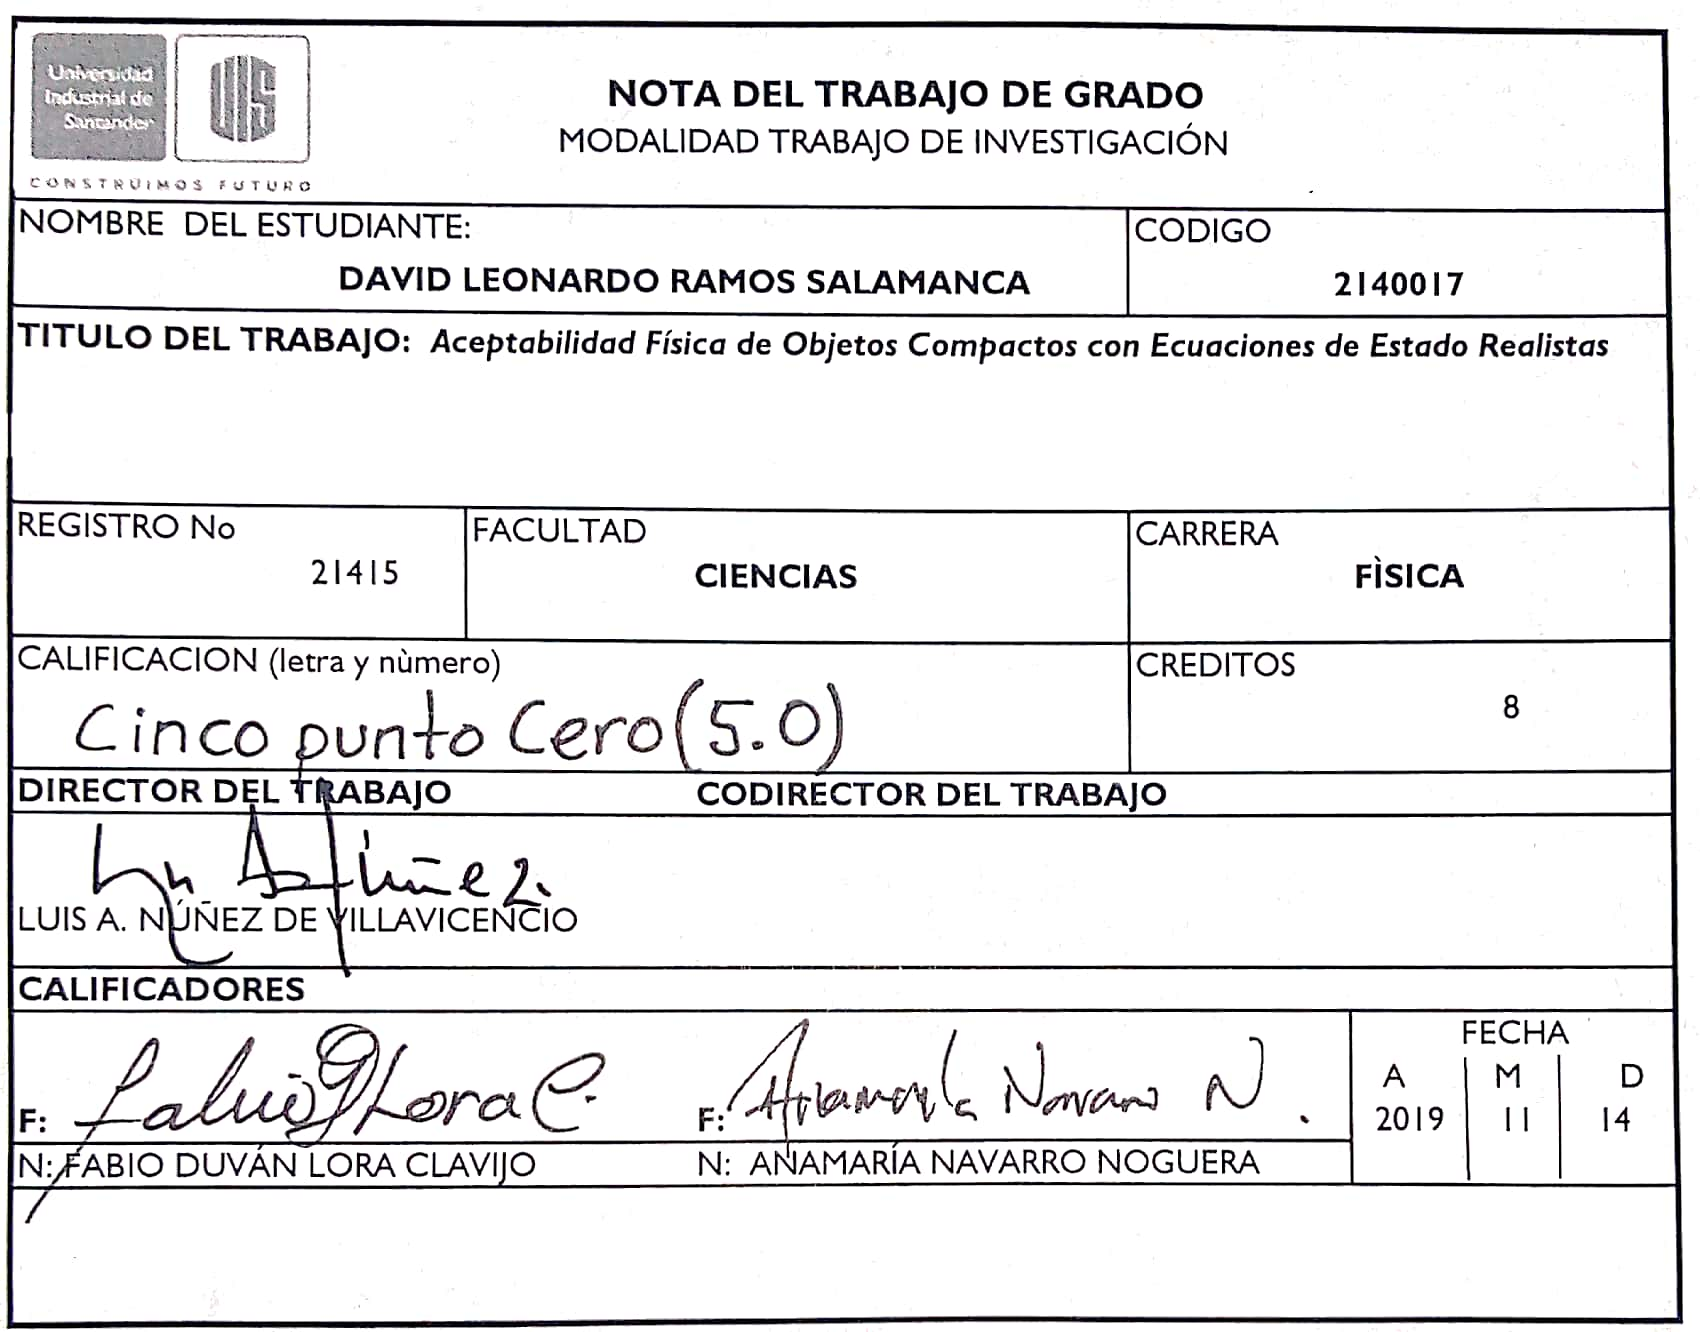
\includegraphics[width=\linewidth]{figures/Nota.jpg}
\end{center}
\newpage

\begin{center}
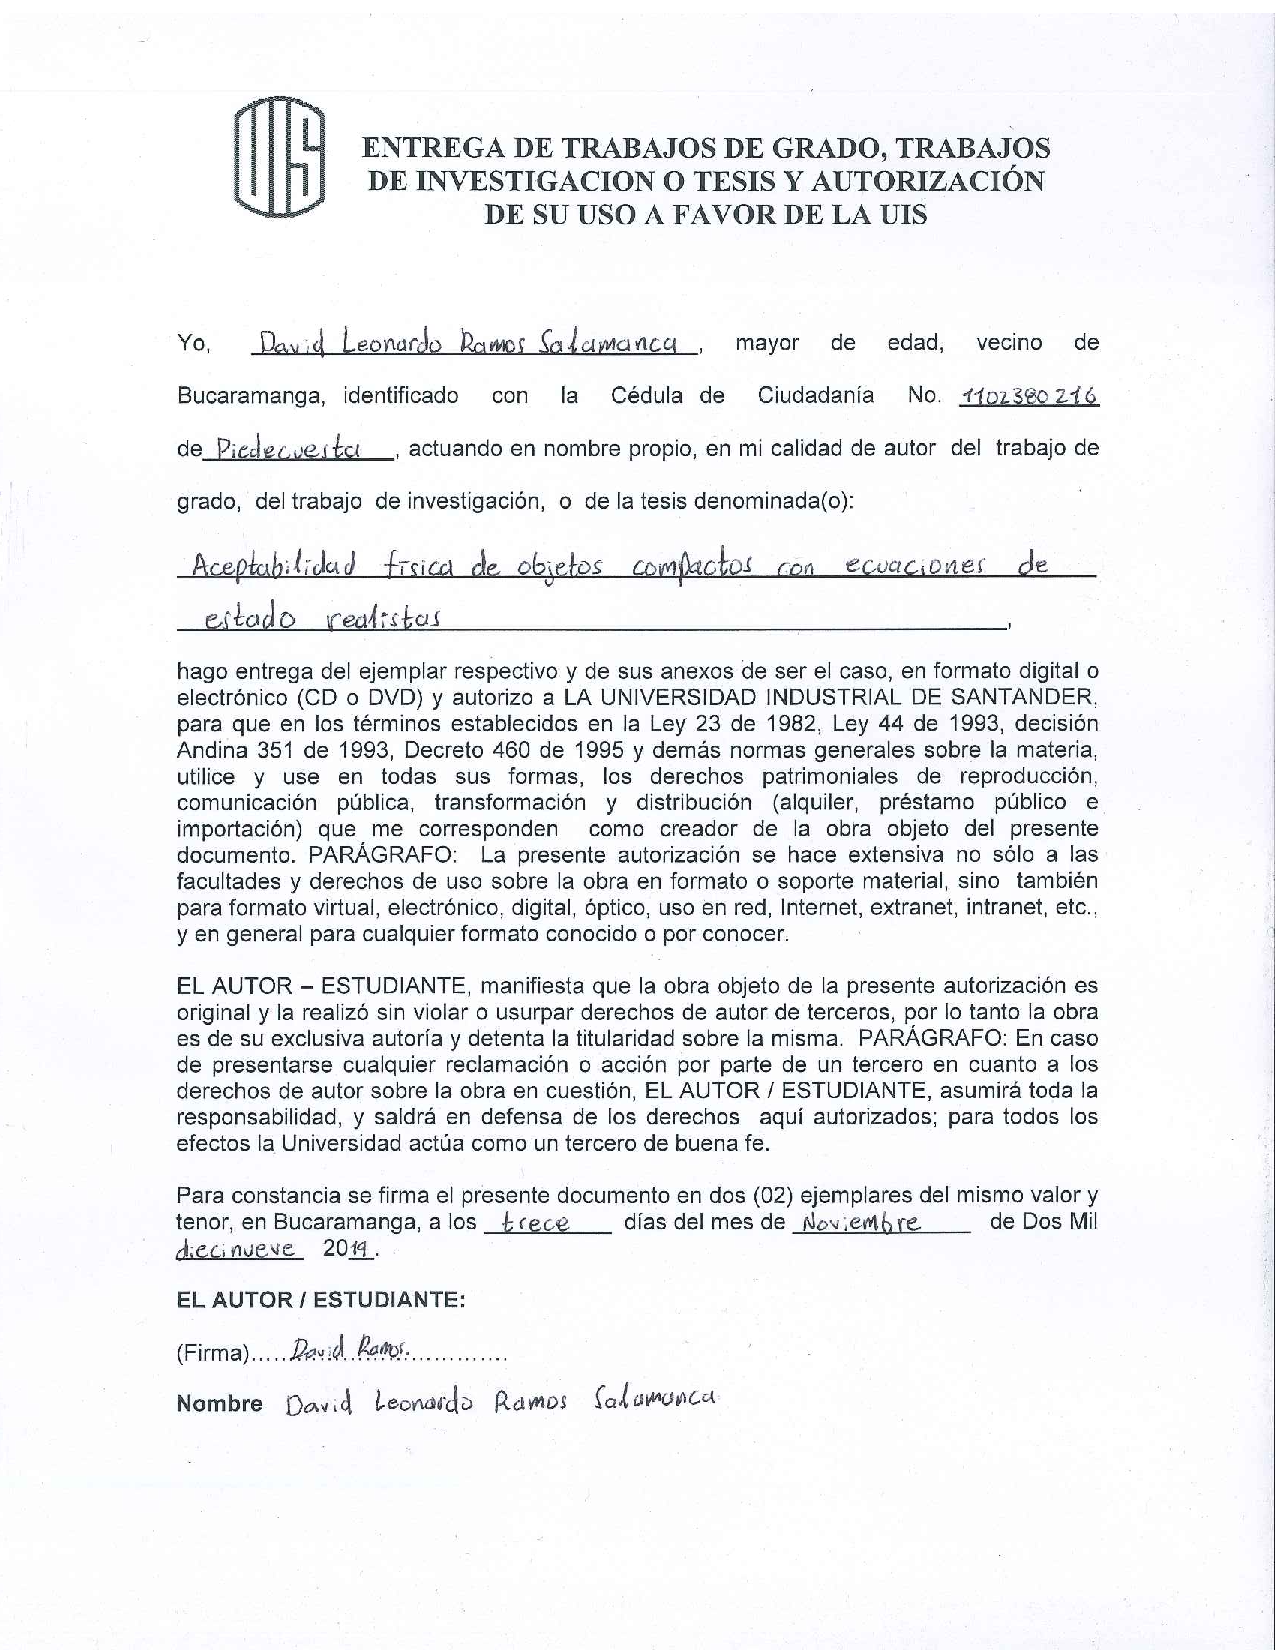
\includegraphics[width=\linewidth]{figures/Autori.pdf}
\end{center}
\newpage

%\begin{acknowledgements}




%\end{acknowledgements}

\newpage
\addtocontents{toc}{\protect\thispagestyle{myheadings}}
\tableofcontents
\addtocontents{toc}{\protect\thispagestyle{myheadings}}
\newpage

\addtocontents{toc}{\protect\thispagestyle{myheadings}}
\listoffigures
\addtocontents{toc}{\protect\thispagestyle{myheadings}}
\newpage 

\addtocontents{toc}{\protect\thispagestyle{myheadings}}
\listoftables
\addtocontents{toc}{\protect\thispagestyle{myheadings}}
\newpage

\newpage


\begin{abstract}
    \begin{spacing}{1.0}
    Los objetos compactos son estrellas tan densas que el uso de la relatividad general es necesario para describir su fenomenología. Debido a que a densidades muy altas la materia está compuesta mayormente de neutrones, estos objetos son conocidos generalmente como estrellas de neutrones. La materia que conforma estas estrellas no puede ser creada en laboratorios terrestres y constituyen por lo tanto un laboratorio astrofísico ideal para verificar teorías físicas de materia densa.
    
    Modelar el interior de las estrellas de neutrones ha requerido superar una gran cantidad de retos teóricos en física nuclear. Tanto así que encontrar la ecuación de estado que gobierna la materia en tales condiciones es aún uno de los problemas abiertos de la física. Las observaciones de estrellas de neutrones permiten restringir los modelos teóricos usados para obtener la ecuación de estado. Pero la falta de precisión en las mediciones no ha permitido identificar la teoría correcta, de modo que características fundamentales como la composición precisa de la materia al interior de la estrellas de neutrones sigue en debate. 
    
    En este trabajo se propuso usar criterios de \quotes{aceptabilidad física} (consideraciones de consistencia física y estabilidad dinámica) para restringir los modelos de materia ultradensa existentes. En particular, se hizo énfasis en aplicar rigurosamente los criterios de estabilidad conocidos. Como resultado, se encontró que todos los modelos estelares encontrados con las ecuaciones de estado que se consideraron, no cumplen un simple criterio de estabilidad ante movimientos convectivos formulado recientemente por Hernandez et al. \cite{Hernandez2018}.
    \end{spacing}
\end{abstract}
\newpage
\begin{abstract1}
    \begin{spacing}{1.0}
    Compact objects are stars so dense that general relativity is required to describe their phenomenology. These are commonly known as neutron stars due to the fact that at very high densities matter is largely composed of neutrons. The matter inside these stars cannot be recreated in terrestial laboratories and this makes them an ideal astrophysical laboratory to test theories of dense matter.
    
    Modelling the interior of neutron stars has required to overcome several theoretical challenges in nuclear physics. So much so that finding the equations of state that describes matter in such conditions is still one of the open problems in physics. Observations of neutron stars can constraint the theoretical models used to obtain the equation of state. But the lack of precision hasn't allowed to identify the correct theory, in such a way that fundamental characteristics as their composition are still up to debate.
    
    Here we propose using \quotes{physical acceptability} criteria (considerations of physical consistency and stability) to constraint existing ultradense matter models. In particular, the rigurous use of known stability criteria was emphasized. As a result, we found that all stelar models constructed with the equations of state considered do not satisfy a simple stability criterion against convective motion proposed recently by Hernandez et al. \cite{Hernandez2018}.
    \end{spacing}
\end{abstract1}

\mainmatter % do not remove this line

% Start writing here-------------------------------------------

\chapter*{\hspace*{6.5cm}Introducción}
\addcontentsline{toc}{chapter}{Introducción}

\noindent Las estrellas de neutrones son las estrellas más densas del universo: una estrella de neutrones estándar tiene una masa $M= 1.4\,M_{\odot}$ y un radio $R=10\,\text{km}$, lo cual implica que su densidad promedio es $\bar{\rho}=(2-3)\rho_0$ donde $\rho_{0}=2.3\times 10^{14} \text{g cm}^{-3}$ es la densidad de la materia nuclear en un núcleo atómico pesado. 

Estas estrellas tan densas fueron anticipadas por Landau en 1932 \cite{Yakovlev2013} y predichas por Baade y Zwicky en 1934 \cite{Baade1934} como el destino final de estrellas masivas que liberan grandes cantidades de energía en explosiones de supernova. Tolman y Oppenheimer \& Volkoff en 1939 \cite{Tolman1939,Oppenheimer1939} fueron los primeros en reconocer la necesidad de estudiar objetos tan densos como las estrellas de neutrones en el contexto de la relatividad general y derivaron la ecuación de equilibrio hidrostático para una estrella estática con simetría esférica. Después de dos décadas de intentos fallidos de observarlas y avances teóricos en el tema: la construcción de las primeras ecuaciones de estado que describían la materia nuclear densa, la predicción de superfluidez de la materia nuclear y el desarrollo de modelos de enfriamiento por emisión de neutrinos y radiación térmica. Las estrellas de neutrones fueron descubiertas finalmente por Jocelyn Bell en 1967 \cite{Hewish1968} en forma de pulsares: estrellas de neutrones rotantes altamente magnetizadas.

Desde entonces, las estrellas de neutrones se convirtieron en un laboratorio astrofísico que permite probar las teorías físicas desarrolladas en múltiples disciplinas a condiciones extremas que no son realizables en los laboratorios terrestres. Comportamientos exóticos como campos magnéticos con magnitudes muy grandes (de $10^4$ a $10^{11}$ T), opacidad a neutrinos y materia dominada por hiperones o quarks desconfinados, son exclusivos de las estrellas de neutrones y su descripción ha planteado retos teóricos importantes. El más grande de estos retos reside en encontrar la ecuación de estado (de aquí en adelante EOS) de la materia al interior de las estrellas de neutrones. 

Numerosos modelos de EOSs han sido desarrollados a lo largo de las últimas dos décadas basados en diferentes enfoques teóricos que son usados para extrapolar de manera consistente nuestro conocimiento de la materia nuclear a sistemas con densidades tan altas (el estado del arte en el tema es presentado en las revisiones \cite{Ozel2016,Oertel2017} y libros \cite{Haensel2007,Rezzolla2018}). El enfoque que más ha sido usado para (des)favorecer modelos de EOSs es el uso de observaciones para restringir los valores de la masa máxima y el radio típico de las estrellas de neutrones (ver \cite{Lattimer2019} para una revisión reciente del tema). Sin embargo, ante la posible existencia de varios modelos que satisfagan las restricciones observacionales esta metodología puede tener un alcance limitado.   

Un enfoque distinto para restringir los modelos de EOSs, inspirado en lo realizado en el campo de las soluciones exactas a las ecuaciones de Einstein en relatividad general (ver \cite{Delgaty1998} por ejemplo), es usar condiciones de regularidad, consistencia y estabilidad físicas para evaluar si los modelos estelares (soluciones a las ecuaciones de Einstein) obtenidos usando un modelo determinado de EOS, son físicamente plausibles. Recientemente uno de estos criterios fue usado satisfactoriamente para restringir EOSs en \cite{Koliogiannis2019a}.

Teniendo en cuenta lo anterior, este trabajo de grado tiene como objetivo emplear este enfoque aplicando el conjunto de condiciones de aceptabilidad reunido por B. Ivanov \cite{Ivanov2017} para el caso de un fluido anisótropo y extendido por Hernández et al. \cite{Hernandez2018}, a modelos de estrellas de neutrones estáticas obtenidos con EOSs disponibles en la literatura (se usará la elección presentada en \cite{Ozel2016}). El resultado será una exhaustiva clasificación de la aceptabilidad física de una parte de las EOSs disponibles. Esta clasificación podrá ser fácilmente verificada y extendida, ya que tanto las rutinas numéricas construidas para crear los modelos como el análisis de estos fue realizado usando software libre y se encuentra disponible como un repositorio público en Github\footnote{\url{https://github.com/DavidRamosSal/stellar_structure}}. Se corroborará además, que esta metodología es efectiva para identificar potenciales problemas con los modelos de EOSs existentes. 
%\REMARK{No sé qué citas poner aquí profe.}

Este trabajo estará organizado de la siguiente manera: en el Capítulo 1 se presentarán algunas generalidades de las estrellas de neutrones, con el fin de sintetizar parte del conocimiento que tenemos de ellas, cómo lo obtenemos y sus grandes limitaciones. En el Capítulo 2 se planteará una forma distinta de evaluar los modelos de EOSs existentes: tras mostrar cómo se crean modelos estelares de estrellas de neutrones, se enunciarán las condiciones de aceptabilidad física que los modelos estelares de cualquier modelo de EOS debe cumplir. El capítulo 3 sirve como una documentación de la rutina numérica usada para construir los modelos estelares a partir de una EOS tabulada así como del cálculo de las derivadas numéricas. En el Capítulo 4 se presentarán los resultados de aplicar las condiciones a los modelos de estrellas de neutrones obtenidos con 37 EOSs de estado realistas con distintas características y se discutirá lo encontrado para cada condición. Finalmente, en el Capítulo 5 se encuentran las conclusiones del trabajo y posibles direcciones de trabajo a futuro. Los apéndice incluido tiene como propósito presentar una deducción de la curvatura para un espacio-tiempo estático con simetría esférica usando el formalismo de Cartan así como la deducción de la solución exterior de Schwarzchild y de las ecuaciones de Tolman-Oppeinheimer-Volkoff. 


\chapter{Estrellas de neutrones: lo que sabemos}

\noindent En este capítulo se resumirán algunos aspectos de nuestro conocimiento actual de las estrellas de neutrones. Comenzando por cómo son formadas, describiendo las regiones interiores que se conocen relativamente bien y mencionando las hipótesis respecto a la composición de su núcleo. Finalmente se presentarán algunas de las manifestaciones observacionales más importantes de las estrellas de neutrones.


\section{De estrellas normales a estrellas de neutrones}

\noindent Las estrellas son formadas a partir de nubes de gas interestelar, compuestas en su mayoría de hidrógeno molecular, que debido a algún tipo de perturbación comienzan a colapsar gravitacionalmente. La compresión del gas incrementa su temperatura hasta que la presión es capaz de balancearla, alcanzando el equilibrio hidrostático. Este equilibrio es temporal debido a que la pérdida de energía (en forma de radiación) disminuye la temperatura del gas y la consecuente reducción de la presión permite que la contracción continúe. El proceso de contracción y equilibrio del material se repite durante un periodo de tiempo (fase pre-secuencia principal), hasta que la temperatura aumenta lo suficiente para que la fusión de hidrógeno en helio pueda ocurrir en el núcleo ($T\approx 10^7\,\si{\kelvin}$). Este proceso de fusión nuclear compensa las pérdidas radiativas y mantiene a la estrella en un equilibrio hidrostático estable \cite{Scilla2016}.

Las reacciones nucleares pueden sostener a la estrella durante la mayor parte de su vida luminosa (de millones a billones de años, dependiendo de su masa inicial \cite{Salaris2005}). Estrellas en esta fase forman la secuencia principal del diagrama de Hertzsprung-Russell.

\setcounter{footnote}{0}
\begin{figure}[H]
    \centering
    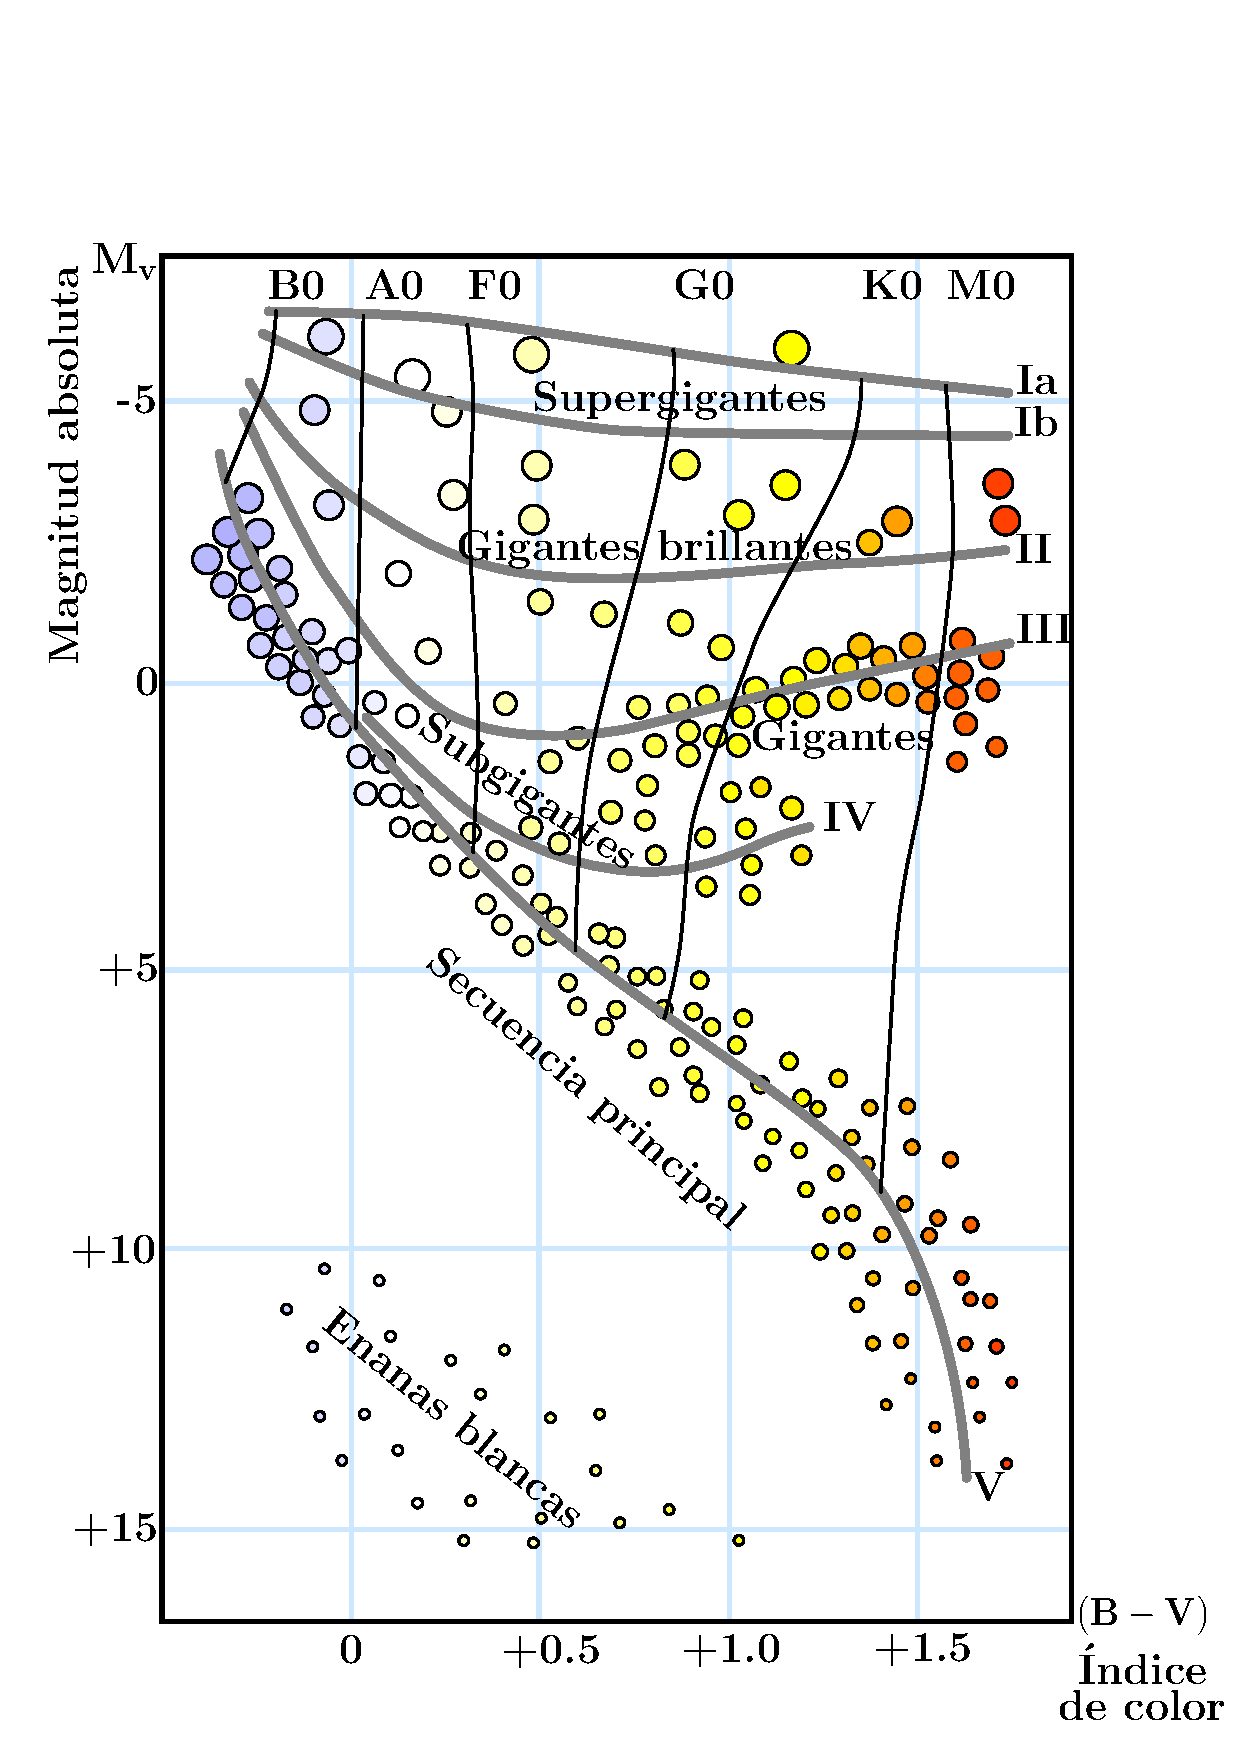
\includegraphics[width=205pt]{figures/H-R_diagram.pdf}%
    \caption[Diagrama Hertzsprung-Russell]{Diagrama Hertzsprung-Russell.\protect\footnotemark}
    \label{HR}
\end{figure}
\footnotetext{Adaptado de \url{https://commons.wikimedia.org/wiki/File:H-R_diagram.svg}}

La evolución de la estrella después de agotar el hidrógeno depende de su masa: estrellas con \emph{masas pequeñas e intermedias} ($M\leq M_{\odot}$) procederán a fusionar helio formando carbono en su núcleo. Esto representa una transición de la secuencia principal hacia la rama de gigantes (hacia el rojo) en el diagrama de Hertzsprung-Russell. Durante las últimas etapas de evolución, estas estrellas liberan sus capas más externas formando una nebulosa planetaria y dejando un núcleo que será sostenido por la presión de degeneración de electrones, conocido como una enana blanca \cite{Padmanabhan2000}.




Estrellas \emph{masivas} ($M>8 M_{\odot}$) entran en un ciclo de fusión de elementos en su núcleo, formando elementos cada vez más pesados (helio, carbono, oxígeno, magnesio, silicio y hierro) \cite{Glendenning2000}. Al final de cada una de estas etapas de fusión los elementos pesados recién creados formarán un núcleo, y los restos del elemento ligero forman un cascarón a su alrededor. En el diagrama de Hertzsprung-Rusell estas estrellas llegarán hasta la parte superior de la secuencia principal y se moverán hacia la rama de supergigantes. Al alcanzar el hierro, la fusión deja de ser exotérmica (en lugar de liberar energía, requerirá de esta) y deja a la estrella sin una fuente de energía que mantenga el equilibrio hidrostático. Estas estrellas colapsarán eventualmente en un evento conocido como supernova (de colapso de núcleo), en este evento los cascarones de los distintos elementos caen sobre el núcleo de hierro desencadenando, mediante mecanismos que no han sido enteramente comprendidos \cite{Janka2012}, la eyección de gran parte de su masa en una explosión \cite{Woosley2005}.

Tras la supernova, el núcleo colapsado \cmmt{ —cuya composición precisa no se conoce pero se presume contiene neutrones, protones, mesones, hiperones e incluso quarks desconfinados—}  inicia un proceso de enfriamiento y reajuste estructural, durante el cual emite una gran cantidad de energía en forma de radiación y neutrinos (importantes a la hora de verificar modelos teóricos, ver por ejemplo \cite{Alvarez-Salazar2018}). Después de alcanzar una composición estable —no conocida con precisión pero se presume contiene neutrones, protones, mesones, hiperones e incluso quarks desconfinados \cite{Lattimer2004}— la presión de degeneración de sus componentes y la repulsión de rango corto entre nucleones sostendrán el núcleo colapsado \cite{Glendenning2000}, alcanzando una estructura definida conocida generalmente como un objeto compacto o estrella de neutrones.
\section{Observaciones}\label{ObsMan}
\noindent Las estrellas de neutrones se manifiestan observacionalmente en una variedad de formas. Esto les permite ser observadas no solo en todas las bandas del espectro electromagnético, sino en eventos de ondas gravitacionales. En esta sección se discutirá brevemente dos de sus principales manifestaciones observacionales: los pulsares y la radiación térmica, comúnmente usadas para medir masas y radios, respectivamente.

\subsection{Pulsares}

\noindent Los pulsares son estrellas de neutrones magnetizadas que rotan emitiendo radiación desde la magnetósfera, orientada principalmente en los polos magnéticos, a expensas de su energía rotacional \cite{Becker2009}, estos son detectados cuando uno de estos rayos cruza la tierra. La mayoría de las estrellas de neutrones conocidas son observadas como pulsares con un espectro en el rango del radio. Aunque la mayoría de pulsares de radio están aislados, una pequeña cantidad de pulsares pertenecen a sistemas binarios los cuales son de suma importancia ya que todos los métodos para medir la masa de los pulsares están basados en el trazado del movimiento orbital del sistema usando el tiempo de llegada de los pulsos observados \cite{Ozel2016}.

%\TODO{Quizá listar los métodos que usan a los pulsares}

\subsection{Emisión térmica}

\noindent Una parte apreciable de la radiación emitida por estrellas de neutrones aisladas parece ser radiación térmica originada cerca a su superficie \cite{Potekhin2010}. Esta radiación es emitida principalmente en los rayos X blandos y múltiples técnicas de espectroscopía se han desarrollado para obtener restricciones sobre los radios de estrellas de neutrones \cite{Ozel2016}.

%\TODO{Listar métodos que usan radiación térmica para medir el radio}

Recientemente se ha identificado que las curvas de enfriamiento (dependencia temporal de la luminosidad detectada por un observador lejano) proveen una manera de caracterizar la estructura interna de las estrellas, \cite{Yakovlev2004}. Sin embargo en estrellas de neutrones que no están aisladas, otras fuentes de rayos X como la acreción dominan y ha sido difícil usar este método para complementar las mediciones en sistemas binarios \cite{Potekhin2010}.


\section{Ecuación de estado}\label{EOS}

\noindent Como se verá en la Sección \ref{SMABC}, la ecuación de estado de la materia es necesaria para crear modelos estelares. Esta se determina predominantemente de la interacción nuclear fuerte entre los constituyentes elementales de la materia. Aunque la ecuación de estado de las estrellas de neutrones sigue siendo un misterio, debido a que estas interacciones no son bien entendidas en materia a densidades superiores a la densidad de saturación nuclear $\rho_0$ \cite{Haensel2007}, existe una gran variedad de EOSs basadas en diferentes métodos de muchos cuerpos usados para describir la materia nuclear. Los métodos de muchos cuerpos se dividen en dos grupos principales: los métodos microscópicos y los modelos fenomenológicos \cite{Rezzolla2018,Giai2010}.

Los \emph{modelos microscópicos} empiezan con interacciones neutrón-neutrón, ajustadas a datos experimentales de dispersión de neutrones y a partir de ella se obtiene la EOS usando un esquema de muchos cuerpos \cite{Ring1980}. Los modelos más comunes de este tipo están basados en el método de Dirac-Brueckner Hartree-Fock (BD-HF) o en el método variacional.

Los \emph{modelos fenomenológicos} se basan en interacciones efectivas dependientes de parámetros que pueden ajustarse para reproducir las propiedades de la materia nuclear conocidas \cite{Baldo2012}. Este tipo de modelos puede ser no-relativista (basados en un Hamiltoniano para el sistema de muchos cuerpo con un potencial de interacción efectivo tipo Skyrme o Gogny) o relativista (basados en un Lagrangiano efectivo con bariones y mesones) y usan la teoría del funcional de densidad de energía (EDF) para reproducir las propiedades de nucleos conocidos.

Una revisión general del estado del arte de las EOS para estrellas de neutrones, además de detalles sobre los modelos mencionados puede encontrarse en las referencias \cite{Haensel2007,Rezzolla2018}.


\section{Estructura interna}\label{IntStr}
A pesar de que sus más importantes características no han sido predichas unívocamente ($M_{\text{max}}$ y $R_{1.4}$), debido a su sensible dependencia de la EOS de la materia nuclear ultradensa, %al reto teórico que representa obtenerla a partir de una teoría relativista de muchos cuerpos para partículas que interactúan fuertemente,
la EOS en regiones con densidades menores a $\rho_0$ se conocen con la suficiente precisión \cite{Haensel2007,Chamel2008} para reconocer características generales de su estructura interna. 

\begin{figure}%[H]
    \centering
    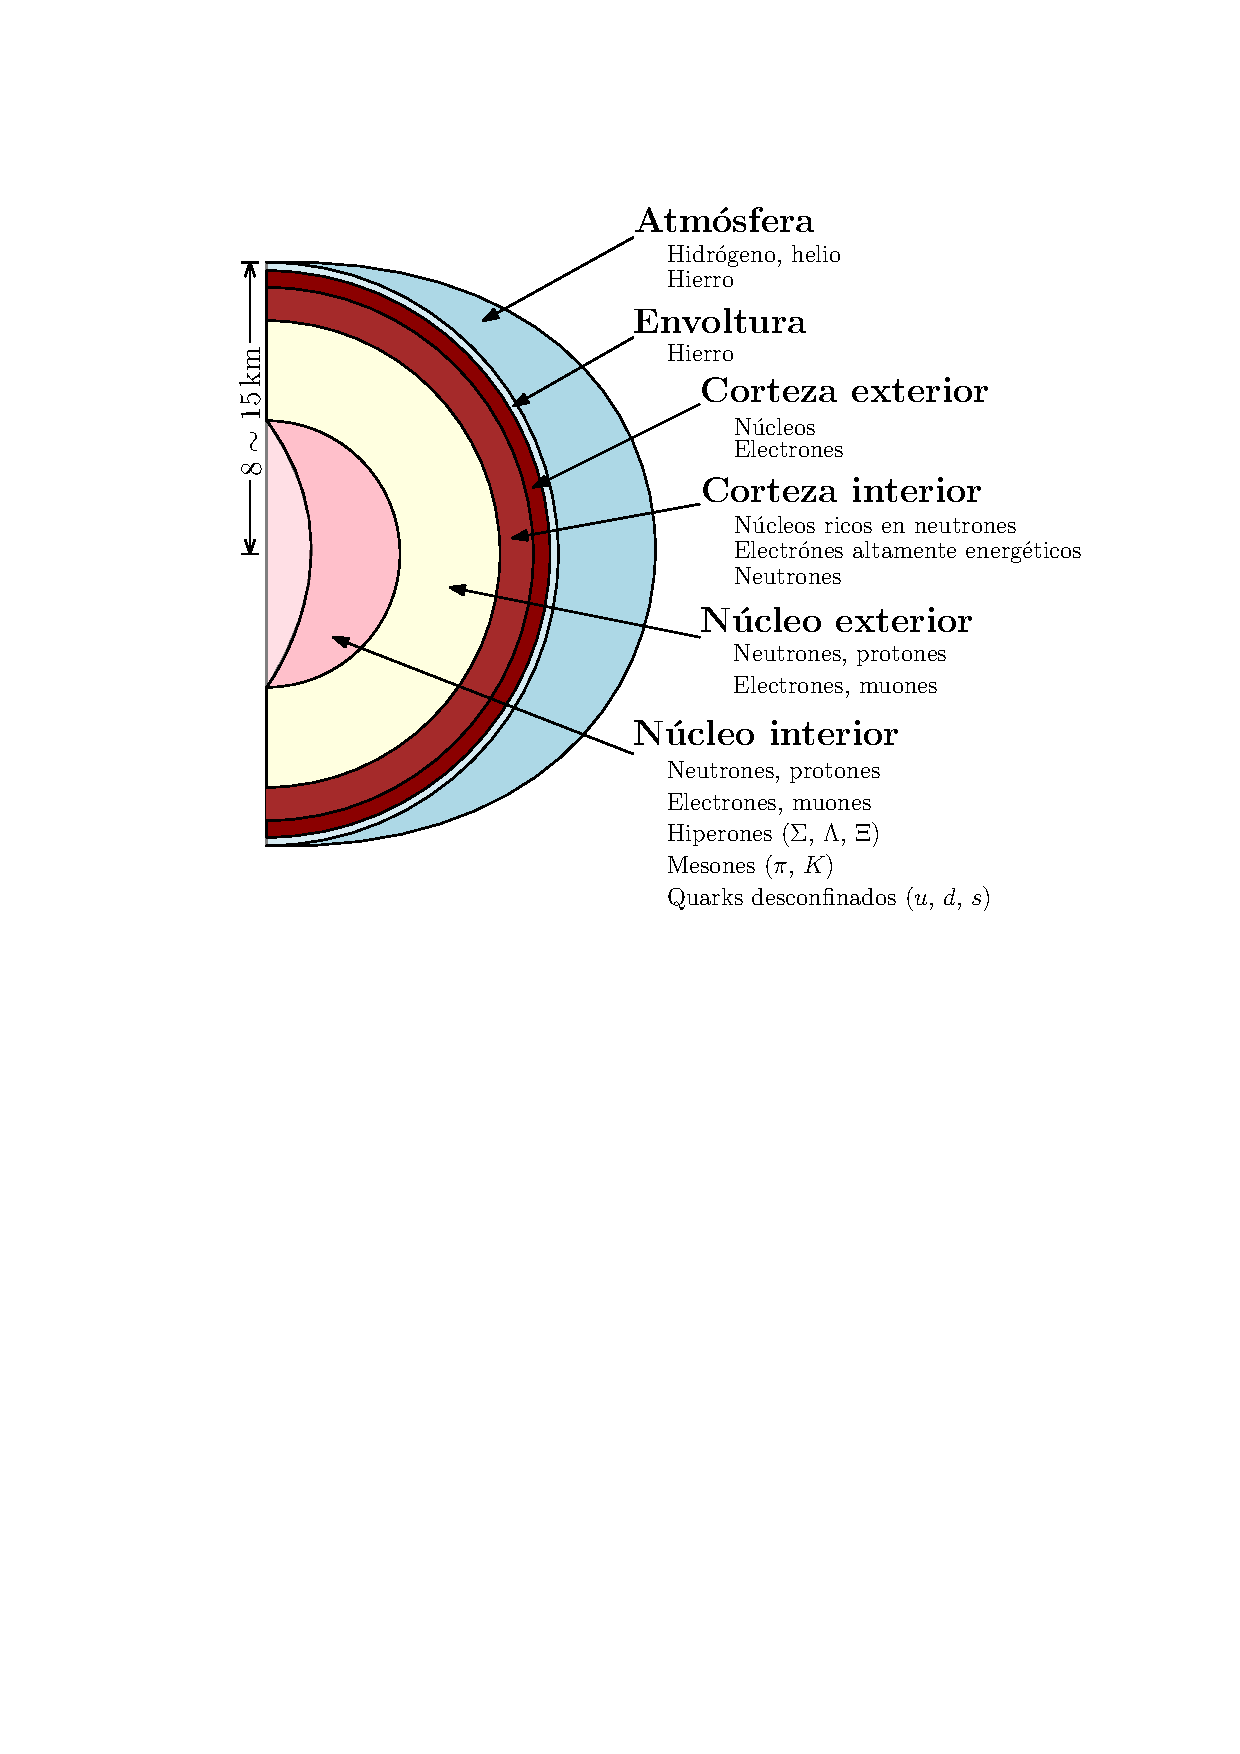
\includegraphics[width=300pt]{figures/neutronstar.pdf}
    \caption[Composición de una estrella de neutrones]{Composición de una estrella de neutrones.\protect\footnotemark}
    \label{NSC}
\end{figure}
\footnotetext{Adaptado de \cite{Weber2012}, Figura 1.}



\noindent La composición de las estrellas de neutrones, contrario a lo que el nombre sugiere, se presume es muy rica y varía a lo largo de su extensión radial. Esta variada composición y las distintas fases que exhiben, están distribuidas en una estructura de cascarones, denominada generalmente una red cristalina de Coulomb (ver Figura \ref{NSC}).
La superficie de la estrella está rodeada por una \emph{atmósfera} compuesta principalmente de hidrógeno, helio y hierro en estado gaseoso o condensado dependiendo de su temperatura superficial y campo magnético \cite{Zavlin2002}. % La atmósfera es importante porque es donde se forma el espectro de radiación electromagnética y éste aporta información acerca de su composición, temperatura y campo magnético.
Bajo la atmósfera se encuentra una \emph{envoltura} (de aproximadamente 100 \si{\metre}), a veces llamado océano. Compuesta presuntamente de núcleos alrededor del pico del hierro en un estado condensado, la envoltura influencia el transporte y emisión de energía térmica desde la superficie \cite{Piekarewicz2013,Potekhin2010,Lattimer2004}.

La envoltura encierra a cuatro regiones internas: la corteza exterior e interior y el núcleo exterior e interior. La \emph{corteza} es una capa en la que se encuentra materia con densidades sub-nucleares ($\rho < \rho_0$). En la \emph{corteza exterior} los electrones presentes, requeridos para la neutralidad de carga de la estrella, forman un gas de Fermi y ocurre un proceso de neutronización donde los electrones son capturados por protones para crear neutrones. La división con la \emph{corteza interior} se presenta debido a que a una densidad $\rho_{ND}\simeq 10^{11}\, \si{\gram\per\centi\metre^2}$ (neutron drip density), los neutrones comienzan a \com{gotear} del núcleo, por lo que hay presencia de neutrones libres, que pueden llegar a condensarse en un superfluido \cite{Baldo2005}. En el fondo de la corteza, cuando la densidad se acerca a $\rho_0$, se ha predicho la presencia de fases conocidas como \com{pasta} nuclear, en las que, debido a la compresión, los núcleos se deforman y dejan de ser esféricos (para una revisión de la corteza de las estrellas de neutrones consultar la referencia \cite{Chamel2008} y referencias allí citadas). 



\begin{figure}[H]
    \centering
    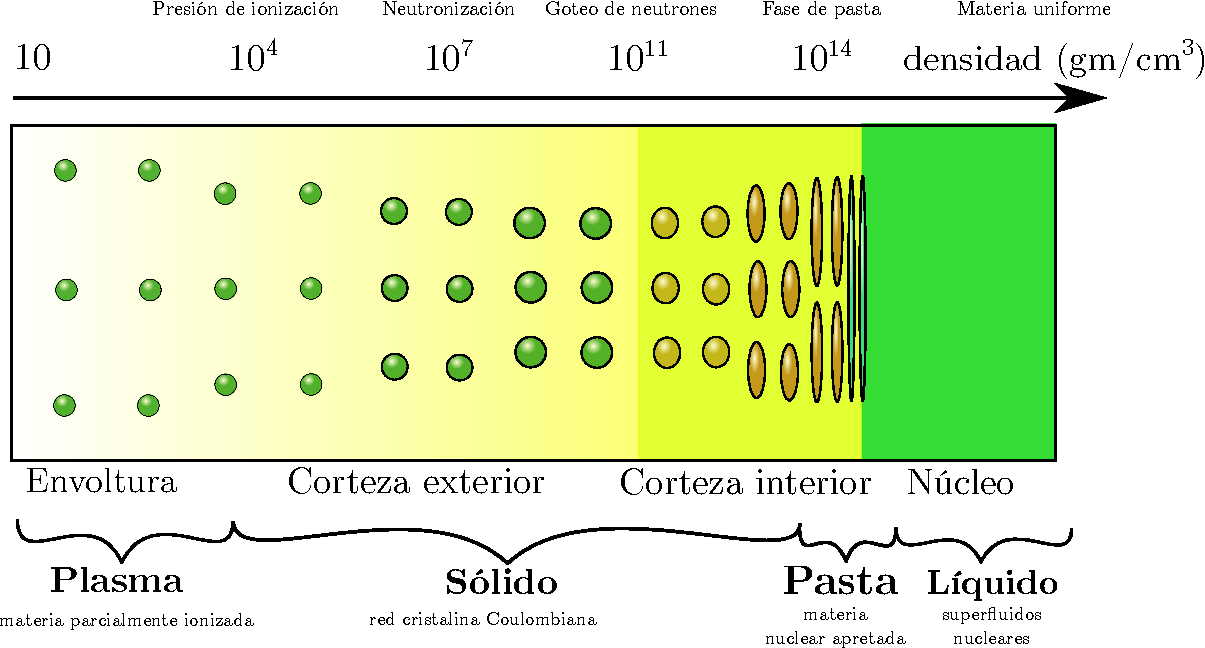
\includegraphics[width=420pt]{figures/Density.pdf}
    \caption[Estructura interna de una estrella de neutrones]{Estructura interna de una estrella de neutrones.\protect\footnotemark}
    \label{NSS}
\end{figure}
\footnotetext{Adaptado de \cite{Chamel2008}, Figura 4.}   

El \emph{núcleo} comprende regiones en las que la densidad alcanza $\rho_0$ y contiene la mayor fracción de la masa estelar. Está subdividido un dos: el \emph{núcleo exterior}, con densidad $\num{0.5}\rho_0\lesssim\rho\lesssim 2\rho_0$  cuya composición se conoce bien cualitativamente \cite{Haensel2007}: es un superfluido de neutrones y protones, con presencia de electrones y muones altamente degenerados. Del \emph{núcleo interior}, por el contrario, no se conoce su composición. Se ha sugerido la presencia de hiperones, piones, kaones e incluso quarks desconfinados (consultar las revisiones \cite{Lattimer2004,Potekhin2010} y referencias allí citadas).

\section{El problema}
Manifestaciones observacionales como las descritas en la Sección \ref{ObsMan} han impuesto restricciones sobre la masa máxima que puede tener una estrella de neutrones y los radios usuales de estas. Como estas características son muy sensibles a la forma precisa de la EOS, las observaciones restringen directamente los modelos de EOSs \cite{Ozel2016}. Sin embargo, se puede argumentar que esta metodología está limitada por el rango de posibilidades físicas consideradas al construir la EOS: si una EOS no se ajusta a las escasas restricciones existentes, la metodología observacional no brinda suficiente información acerca de qué falencias tiene el modelo \cite{Raithel2017}. E incluso en el caso de que un grupo de EOSs cumpla con las restricciones, la metodología observacional no permitiría discernir entre ellas. 

En el siguiente capítulo se propondrá utilizar de manera rigurosa las restricciones que nuestro conocimiento de estructura estelar y relatividad general imponen sobre modelos de estrellas de neutrones. Esto con el propósito de complementar las restricciones observacionales sobre modelos de EOSs.
\chapter{Aceptabilidad física: una alternativa}

\noindent El problema planteado al final del capítulo anterior se puede sintetizar como: no hay suficientes mediciones con la precisión necesaria para identificar la EOS de las estrellas de neutrones unívocamente. En este trabajo se explorará si los requerimientos de consistencia física y estabilidad existentes para modelos de estrellas de neutrones pueden ser útiles para complementar las restricciones observacionales.

Acorde con lo anterior, en este capítulo se desarrollarán las herramientas para crear modelos de estrellas de neutrones estáticas. Seguido de esto se enunciarán las condiciones de aceptabilidad física como los requerimientos mínimos que los modelos obtenidos con cualquier EOS debe cumplir.
%\noindent Explicar la variada fenomenología descrita en el capítulo anterior ha requerido la solución de retos teóricos en ramas tan variadas como la relatividad general, física de la materia condensada y física nuclear. 

%En este capítulo se derivarán las ecuaciones de estructura estelar para una estrella de neutrones fría, neutra, estática y con simetría esférica en la teoría newtoniana y en relatividad general. Después de identificar la necesidad de conocer la EOS de la materia para crear modelos estelares, se  describirá el problema de la EOS de la materia ultradensa y algunos de los métodos usados para hallarla.
%Comparar los dos resultados permitirá identificar algunas de las predicciones de la relatividad general en objetos compactos. 
%Para terminar se enunciará una lista de criterios de consistencia física y estabilidad que los modelos estelares deben cumplir, estos criterios serán usados el siguiente capítulo para evaluar qué tan realistas son los modelos estelares obtenidos con diferentes EOSs.


\section{Modelando de estrellas de neutrones estáticas}

\noindent En esta sección se obtendrán las ecuaciones de estructura estelar para una estrella de neutrones fría, neutra, estática y con simetría esférica en la teoría newtoniana y en relatividad general. Comparar los dos resultados permitirá identificar algunos de los efectos que la relatividad general predice en objetos compactos.

\subsection{Caso newtoniano}

\noindent Considerando una distribución de materia con simetría esférica, si $r$ denota la distancia desde el centro de la configuración, la masa encerrada en una superficie esférica de radio $r$ será:  
\begin{equation}
    m ( r ) = \int _ { 0 } ^ { r } 4 \pi r ^ { 2 } \rho \dd{r} = \int_{0}^{r} \dd{m(r)} \quad\text{con}\quad \dd{m(r)}=4\pi r^2\rho \dd{r},
    \label{mN}
\end{equation}
\begin{equation}
    \Longrightarrow\dv{m(r)}{r} =4\pi r^2 \rho.
    \label{dmnewton}
\end{equation}
Ahora, se considera un cilindro infinitesimal a una distancia $r$ del centro, de altura $\dd{r}$ y sección transversal $\dd{A}$, normal al vector posición $\vec{r}$ (ver Figura \ref{stellnew}).  

Si la presión en $\vec{r}$ es $P$ y su cambio al ir de $\vec{r}$ a $\vec{r}+\dd{\vec{r}}$ es $\dd{P}$. La diferencia de presión representa una fuerza 
\begin{equation*}
    F_{Pelem}=-\dd{P}\dd{A},
\end{equation*}
actuando sobre el elemento de masa.

\begin{figure}[H]
    \centering
    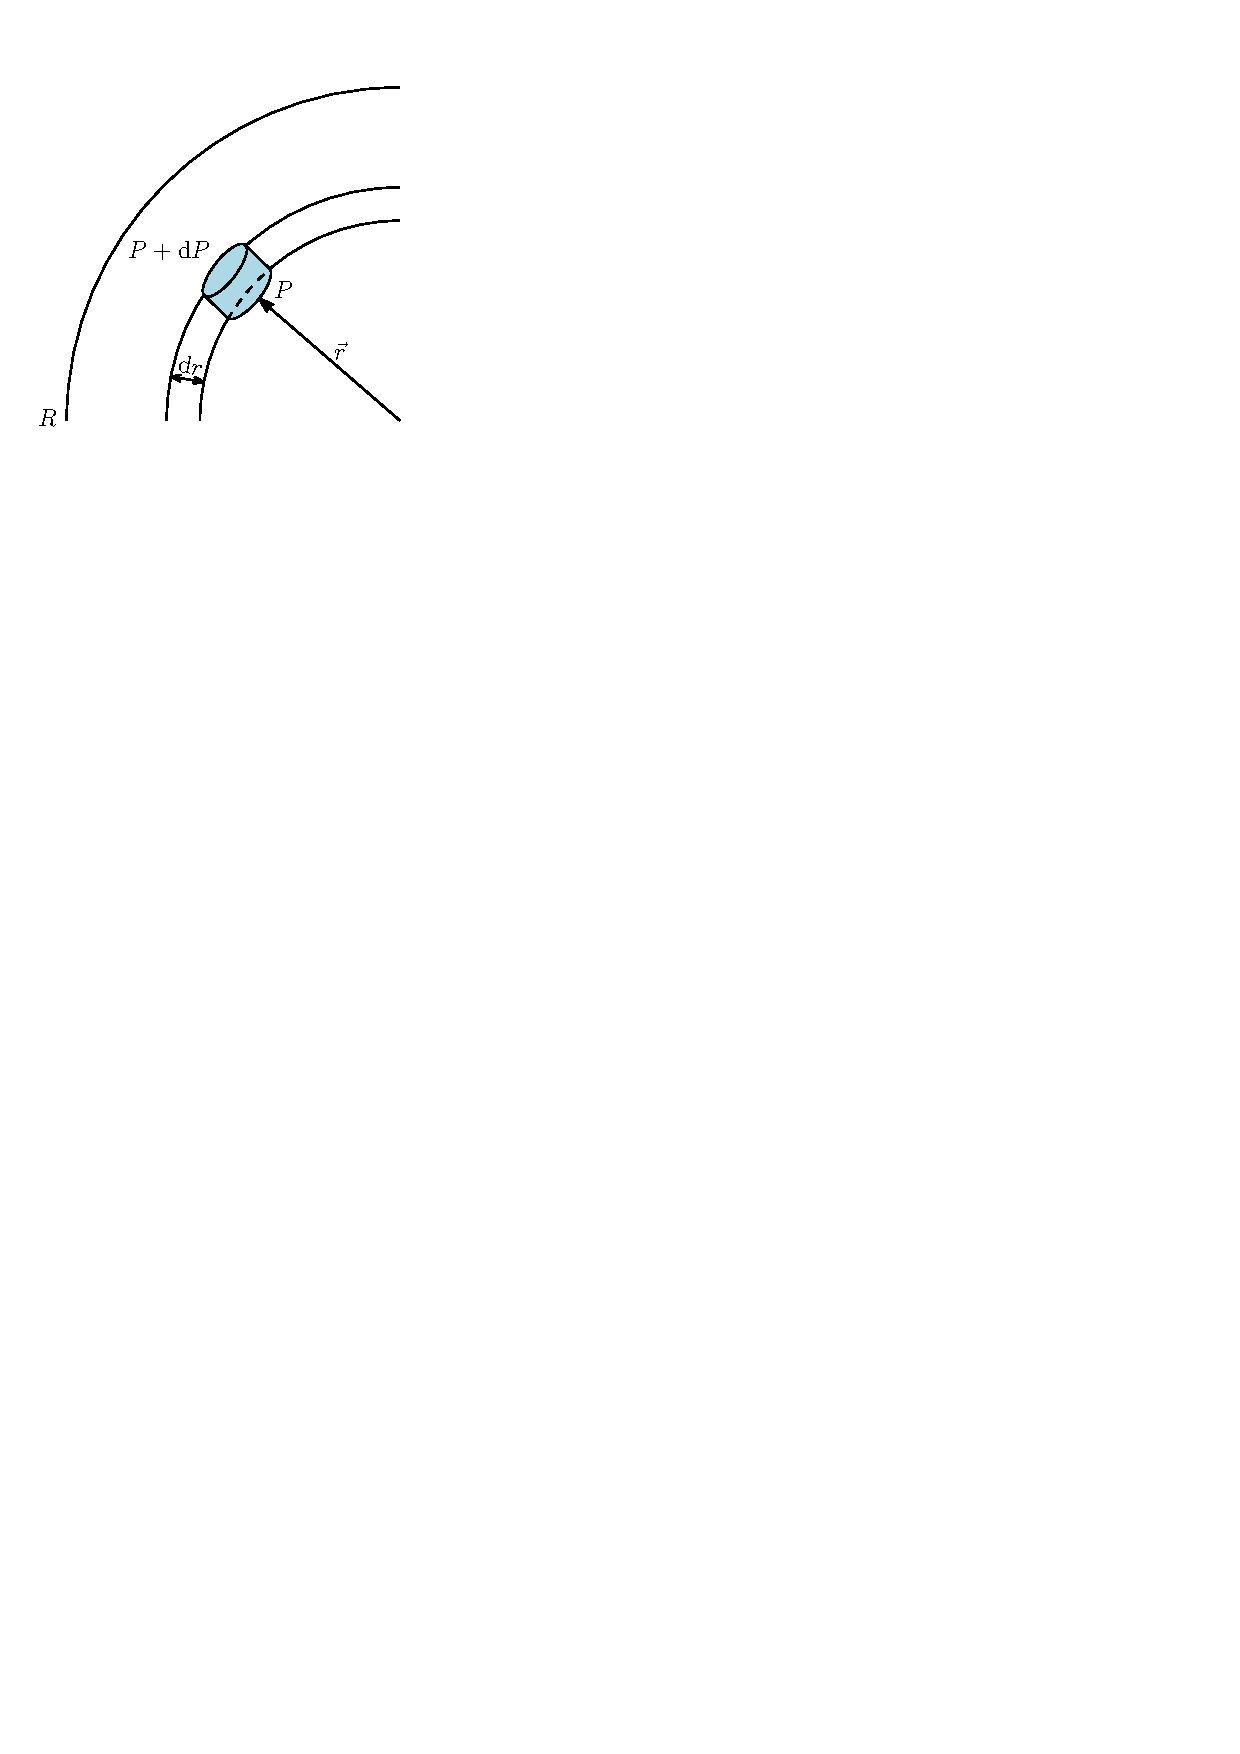
\includegraphics[width=150pt]{figures/stellarnewton.pdf}
    \caption[Presión sobre un elemento de masa cilíndrico]{Presión sobre un elemento de masa cilíndrico.}
    \label{stellnew}
\end{figure}
 Esta fuerza debe contrarrestar la atracción gravitacional sobre el elemento de masa debido a $m(r)$
\begin{equation*}
    F_{atracc}=\frac{G m(r)\rho \dd{A} \dd{r}}{r^2}.
\end{equation*}
Para que el elemento de masa se encuentre en equilibrio se requiere entonces:

\begin{equation}
    -\dd{P}\dd{A} =\frac{G m(r)\rho \dd{A} \dd{r}}{r^2},
\end{equation}
o
\begin{equation}
    \dv{P}{r} = - \frac { G m ( r ) } { r ^ { 2 } } \rho.
    \label{dpnewton}
\end{equation}
que es la conocida ecuación de equilibrio hidrostático. 

Las ecuaciones \eqref{dmnewton} y \eqref{dpnewton} son las ecuaciones de estructura estelar newtonianas \cite{Chandrasekhar1958}. 

%Si una relación entre la presión y la densidad $P(\rho)$ es dada, es decir, una ecuación de estado, el sistema puede resolverse dado un par condiciones iniciales $m(r=0)$ y $P(r=0)$. La primera de estas condiciones es evidente puesto que no hay masa encerrada en un cascarón esférico de radio nulo, $m(r=0)=0$. La segunda estará definida por el valor de $\rho(r=0)\equiv\rho_c$ escogido, mediante la ecuación de estado, $P(r=0)=P(\rho_c)$.

%El radio de la estrella $R$ se define como el valor de $r$ en el que la presión se anula, esto es, $P(R)=0$ y de manera similar la masa de la estrella $M$ se define como el valor de la masa encerrada en $r=R$, esto es, $m(R)=M$.

Aunque no se van a tratar en este trabajo, cabe resaltar que las \emph{enanas blancas}, objetos compactos sostenidos por la presión de degeneración de electrones, pueden ser descritas por las ecuaciones de estructura newtonianas satisfactoriamente. Una manera de conocer la importancia de las correcciones relativistas de una estrella es comparando el valor de la compacidad de la estrella $\mu \equiv \frac{2GM}{c^2R}$ con la unidad (la razón será evidente en el resultado relativista) \cite{Weinberg1972}. Las enanas blancas tienen masas en un rango de $0.33\,M_{\odot}$ $1.52\,M_{\odot}$ y radios típicos de unos cuantos miles de kilómetros \cite{Glendenning2000}. Para una enana blanca promedio, con masa $M=0.6\,M_{\odot}$ y radio $r=3000 \,\rm{km}$ se tiene
\begin{equation}
    \mu \simeq 6\times 10^{-4}\ll 1,
\end{equation}
por lo cual se espera que el tratamiento newtoniano sea suficiente. 

\subsection{Caso relativista}\label{CR}
%\TODO{Basado en los comentarios de la propuesta modificar esta sección. Teniendo en cuenta que los cálculos están hechos en el apéndice.}

%Si bien en la teoría newtoniana podrían existir objetos tan compactos como las estrellas de neutrones, algunas de las predicciones presentan inconsistencias con lo predicho por la teoría de la Relatividad General. Por ejemplo, Chandrasekhar encontró (usando gravedad newtoniana) que las estrellas soportadas por presión de degeneración tienen una masa máxima, obtenida asintóticamente cuando los fermiones son altamente relativistas. Esto es, cuando tienen velocidades comparables con la velocidad de la luz. Bajo tales condiciones la teoría newtoniana permitiría la existencia de estrellas compuestas por los quarks más pesados (charm, bottom y top). En Relatividad General se predice también la existencia de una masa máxima, pero ésta no es de naturaleza asintótica sino que está inmersa en la forma de las ecuaciones de estructura estelar. Las estrellas con la mayor masa posible en Relatividad General, en contraste a lo predicho por la teoría newtoniana, no son lo suficientemente densas para permitir la presencia de los quarks más pesados \cite{Glendenning2000}.

%Predicciones contradictorias como la anterior favorecen a la Relatividad General en el estudio de objetos compactos, pues ésta ha explicado fenómenos como la precesión de mercurio, que no pueden ser explicados en gravedad newtoniana (ver  \cite{Turyshev2008ExperimentalRelativity} para una revisión de tests experimentales de la Relatividad General).

\noindent\small{\textbf{Nota:} a lo largo de esta sección se hará uso del convenio de suma de Einstein y de unidades gravitacionales ($G=c=1$), excepto en donde sea explícitamente especificado. Además, las primas representan derivada con respecto a $r$ y se usará esta notación indistintamente con la notación diferencial.}
\normalsize

\noindent Para describir la estructura de una estrella estática en Relatividad General se supone un espacio-tiempo asintóticamente plano, estático y con simetría esférica, descrito de manera general por el elemento de linea:

\begin{equation}
\dd{s}^ { 2 } = -e ^ { 2 \nu ( r ) } \dd{ t} ^ { 2 } + e ^ { 2 \lambda ( r ) } \dd{ r} ^ { 2 } + r ^ { 2 } \left( \dd{ \theta} ^ { 2 } + \sin ^ { 2 }  \theta  \dd{ \phi} ^ { 2 } \right) .   
\end{equation}

Respecto a una base ortonormal
\begin{equation}
    \omega^0=\,e^{\nu}\dd{t}, \quad
    \omega^1=\,e^{\lambda}\dd{r}, \quad
    \omega^2=\,r\dd{\theta}, \quad
    \omega^3=\,r\sen{\theta}\dd{\varphi},
\end{equation}
el tensor de Einstein asociado a este elemento de linea tiene componentes no nulas (ver el Apéndice \ref{curvature} para la derivación)

\begin{equation}
    \begin{array} { l } { G _ { 0 } ^ { 0 } = e ^ { - 2 \lambda } \left( \frac { 1 } { r ^ { 2 } } - \frac { 2 \lambda ^ { \prime } } { r } \right) - \frac { 1 } { r ^ { 2 } }  }, \\ { G _ { 1 } ^ { 1 } = e ^ { - 2 \lambda } \left( \frac { 1 } { r ^ { 2 } } + \frac { 2 \nu ^ { \prime } } { r } \right) - \frac { 1 } { r ^ { 2 } } }, \\ { G _ { 2 } ^ { 2 } = e ^ { - 2 \lambda } \left( \nu ^ { \prime \prime } + \nu ^ { \prime 2 } - \lambda ^ { \prime } \nu ^ { \prime } + \frac { \nu ^ { \prime } - \lambda ^ { \prime } } { r } \right)  }, \\ { G _ { 3 } ^ { 3 } = G _ { 2 } ^ { 2 }  }, \end{array}
    \label{eee}
\end{equation}

debe satisfacer las ecuaciones de Einstein
\begin{equation}
    G _ { \mu } ^ { \nu }  = 8 \pi T _ { \mu } ^ { \nu },
\end{equation}
fijando así las funciones métricas $\nu$ y $\lambda$, en función del contenido material de la estrella descrito por $T _ { \mu } ^ { \nu }$.

Dividiendo el espacio-tiempo en dos: una región exterior a la estrella y una interior. 
La \textit{región exterior} no tiene fuentes ($T _ { \mu } ^ { \nu }=0$) y las ecuaciones de Einstein para ésta son 
\begin{equation}
    G _ { \mu } ^ { \nu } = 0.
\end{equation}
Este es un sistema de 3 ecuaciones, pues $ G _ { 2 } ^ { 2}=G _ { 3 } ^ { 3}$ y dos incógnitas ($\nu$ y $\lambda$). Las identidades de Bianchi aseguran que una las ecuaciones puede ser escrita en términos de las otras y no brinda información adicional.

Este sistema puede ser resuelto de manera sencilla para obtener (ver el Apéndice \ref{curvature} para una derivación)
\begin{align}
    e^{2\nu}=e^{-2\lambda}=1-\frac{2 M}{r},
\end{align}


que es la conocida solución exterior de Schwarzschild
\begin{equation}
    \dd{s} ^ { 2 } = - \left( 1 - \frac { 2 M } { r } \right) \dd{t} ^ { 2 } + \left( 1 - \frac { 2 M } { r } \right) ^ { - 1 } \dd{r} ^ { 2 }  + r ^ { 2 } \dd{\theta} ^ { 2 } + r ^ { 2 } \sin ^ { 2 } \theta \dd{\phi} ^ { 2 }, \label{schwarzs}
\end{equation}
valida para $r>R$, donde $R$ es el radio de la estrella y $M$ es una constante de integración, que puede ser interpretada como la masa gravitacional al comparar con el límite de campo débil. Este elemento de línea describe la geometría del espacio-tiempo exterior a una estrella estática.

\begin{figure}%[H]
    \centering
    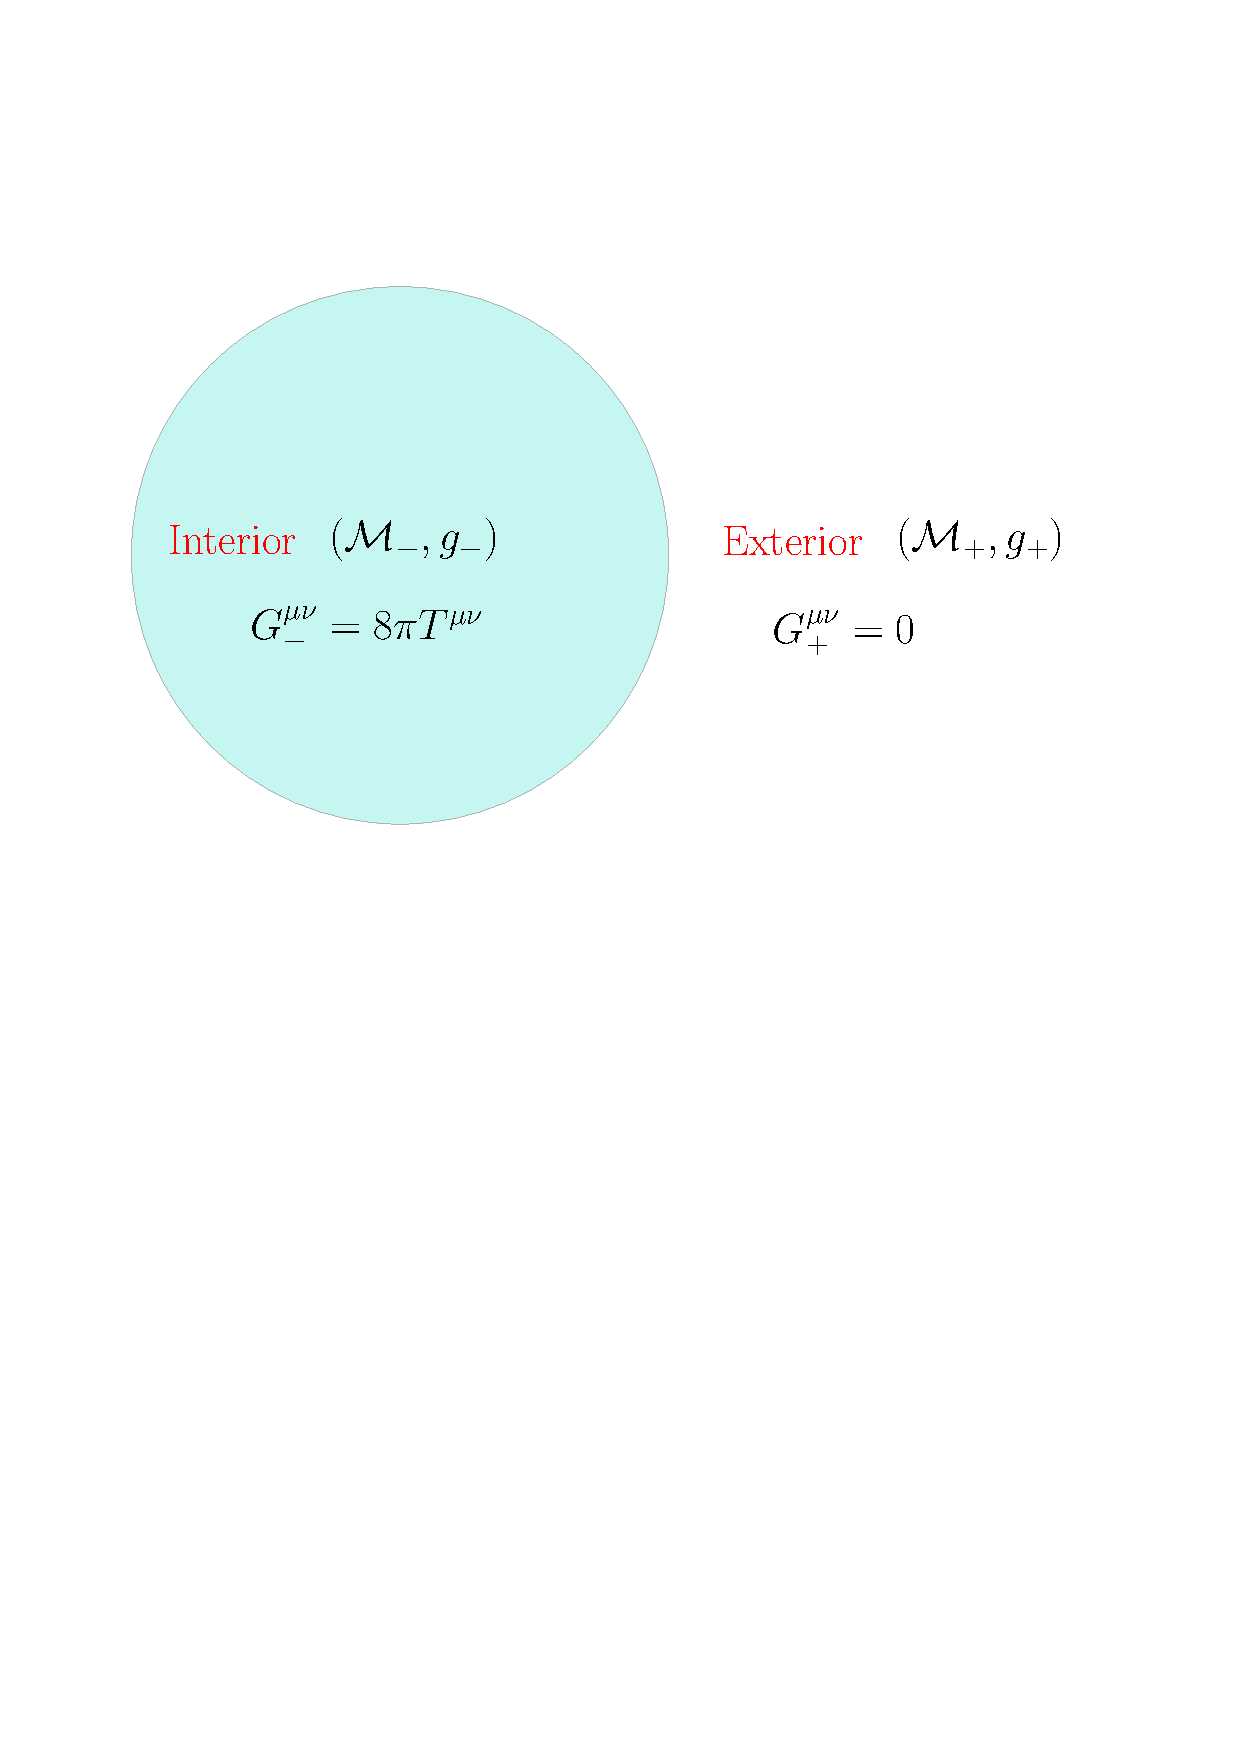
\includegraphics[width=0.7\linewidth]{figures/GR.pdf}
    \caption[División del espacio-tiempo]{División del espacio-tiempo en un espacio-tiempo exterior y un interior. Al asumir que ambos espacio-tiempos son estáticos y tienen simetría esférica las métricas $g_{-}$ y $g_{+}$, así como los tensores de Einstein $G^{\mu \nu}_{-}$ y $G^{\mu \nu}_{+}$ tienen la misma forma.}
    \label{STDiv}
\end{figure}

Para la \textit{región interior} el contenido material debe ser especificado para resolver las ecuaciones de Einstein. Si la materia se modela como un fluido perfecto, el tensor de energía-momento viene dado por

\begin{equation}\label{EMT}
    T ^ { \mu \nu } =  P g ^ { \mu \nu } + ( P + \rho ) u ^ { \mu } u ^ { \nu }
\end{equation}

donde $u^{\mu}=\dv{x^{\mu}}{\tau}$ es la cuadri-velocidad de modo que $g _ { \mu \nu } u ^ { \mu } u ^ { \nu } = -1$ , $P$ su presión y $\rho$ su densidad de energía ambas definidas en un marco comóvil al fluido. Este tensor de energía-momento puede ser deducido del Lagrangiano $L=-\rho$ usando el principio variacional \cite{Felice19992}.

Como se considera una estrella estática, la velocidad espacial de todos los elementos del fluido es cero:
\begin{equation}
    u^{i}=0 \quad (i=1,2,3)\qc u ^ { 0 } = 1
\end{equation}
con lo que las únicas componentes no nulas del tensor energía-momento, en componentes mixtas, serán
\begin{equation}
T _ { 0 } ^ { 0 } = -\rho(r) , \quad T _ { i } ^ { i } =  P(r) \quad ( i=1,2,3 ).  
\end{equation}
Con esta forma del tensor energía-momento y las componentes del tensor de Einstein enunciadas anteriormente, las ecuaciones de Einstein son
\begin{align}
     e ^ { - 2 \lambda } \left( \frac { 1 } { r ^ { 2 } } - \frac { 2 \lambda ^ { \prime } } { r } \right) - \frac { 1 } { r ^ { 2 } } =&  -8\pi\rho, \label{E00} \\
    e ^ { - 2 \lambda } \left( \frac { 1 } { r ^ { 2 } } + \frac { 2 \nu ^ { \prime } } { r } \right) - \frac { 1 } { r ^ { 2 } } =& \, 8\pi P, \label{E11}\\
    e ^ { - 2 \lambda } \left( \nu ^ { \prime \prime } + \nu ^ { \prime 2 } - \lambda ^ { \prime } \nu ^ { \prime } + \frac { \nu ^ { \prime } - \lambda ^ { \prime } } { r } \right) =& \, 8\pi P. \label{E22}
\end{align}

Este sistema de ecuaciones puede ser escrito en una manera más sencilla de integrar usando las Ecuaciones \eqref{E00} y \eqref{E11} suplementadas con la conservación local de la energía y el momento
\begin{equation}
    \qty(\nabla_{\omega_\nu}\mathbf{T})^{\mu \nu} = 0 \label{CEM}.
\end{equation}
La Ecuación \ref{E22} no aportará nueva información pues las identidades de Bianchi aseguran que esta ecuación es una consecuencia de las Ecuaciones \eqref{E00},\eqref{E11} y \eqref{CEM} \cite{Schutz2009}.

Definiendo la variable 
\begin{equation}
     m(r) \equiv \frac{1}{2}r\qty(1-e^{-2\lambda}), \label{misnermass}
\end{equation}
las ecuaciones \eqref{E00}, \eqref{E11} y \eqref{CEM} se reducen al sistema de ecuaciones 
\begin{subequations}
\begin{align}
    \dv{m}{r} &= 4\pi \rho r^2, \label{dmtov} \\
     \dv{P}{r} &= -(P+\rho)\frac{m+4\pi P  r^3}{r\qty(r-2m)},\label{dptov} \\
    \dv{\nu}{r} &= \frac{m+4\pi P   r^3}{r\qty(r-2m)}.\label{dnutov}
\end{align}
\end{subequations}
Las ecuaciones \eqref{dmtov}, \eqref{dptov} y \eqref{dnutov} son las ecuaciones de estructura estelar relativista: describen configuraciones de estrellas de neutrones estáticas en equilibrio. Este sistema de ecuaciones se conoce generalmente como las ecuaciones de Tolman-Oppenheimer-Volkoff (TOV)  \cite{Tolman1939,Oppenheimer1939} y serán referidas de esta manera en adelante. 

Re-escribiendo \eqref{dptov} en unidades SI como
\begin{equation}
    \dv{P}{r} =  - \frac { G  m ( r ) } { r ^ { 2 } } \rho ( r ) \left[ 1 + \frac { P ( r ) } {c ^ { 2 } \rho ( r ) } \right] \left[ 1 + \frac { 4 \pi r ^ { 3 } P ( r ) } { m ( r ) c ^ { 2 } } \right]  \left[ 1 - \frac { 2 G m ( r ) } { c ^ { 2 } r } \right] ^ { - 1 }, 
    \label{dprelat}
\end{equation}
se aprecia que la versión relativista añade correcciones a la ecuación de equilibrio hidrostático newtoniana \eqref{dpnewton} en forma de tres factores adimensionales. Las dos versiones de las ecuaciones de estructura coinciden cuando estos factores se reducen a la unidad, esto es, en el límite cuando 
\begin{equation}
    c^2\rho \gg P \qc mc^2 \gg 4\pi r^3P \quad \text{y} \quad  \frac{2Gm}{c^2r}= \mu \ll 1,
\end{equation}
en un límite no relativista la variable $m$ definida en \eqref{misnermass} (conocida como masa gravitacional)  coincide con la masa Newtoniana \eqref{mN}, además $P$ y $\rho$ varían como $\frac{1}{2}mv^2$ y  $mc^2$ \cite{Silbar2003}. Así, las dos primeras correcciones son de orden $v^2/c^2$ y son válidas cuando las partículas del fluido tienen velocidades pequeñas comparadas con la velocidad de la luz mientras el tercer factor es puramente geométrico. 

Debido a que los tres factores en la ecuación \eqref{dprelat} son mayores que 1, si se compararan dos modelos estelares: uno Newtoniano y otro relativista, que para cierto radio $r$ tienen los mismos valores de $\rho$, $P$ y $m$, la relatividad general predice fuerzas gravitacionales más fuertes sobre la estrella que la teoría Newtoniana. Esto tiene un efecto importante en la estabilidad pues, como se discutirá en la sección \ref{phyacep}, configuraciones que eran estables en la teoría Newtoniana no lo serán en relatividad general. 
%Así pues,  \eqref{dprelat} expresa el \textit{balance} entre la fuerza neta sobre un elemento de masa debido a la presión de la materia que la rodea y la atracción gravitacional de la materia interior a este. Los tres factores en la ecuación \eqref{dprelat} son mayores que 1, esto es, además de la densidad de energía, la presión actúa como una fuente de atracción gravitacional. Esta es la razón por la cual el colapso gravitacional es intrínseco a la estructura de la Relatividad General: mientras en las estrellas newtonianas la presión actuaba para sostener a la estrella, si la estrella es lo suficiente masiva (presiones lo suficientemente grandes) el colapso es inevitable.

\subsection{Cómo construir modelos estelares}\label{SMABC}

\noindent Las ecuaciones de TOV
\begin{align*}
    \dv{m}{r} &= 4\pi \rho r^2, \\
    \dv{P}{r} &= -(P+\rho)\frac{m+4\pi P r^3}{r\qty(r-2m)}, \\
    \dv{\nu}{r} &= \frac{m+4\pi P r^3}{r\qty(r-2m)},
\end{align*}
son un sistema de tres ecuaciones diferenciales ordinarias con cuatro incógnitas $m(r)$, $\rho(r)$, $P(r)$ y $\nu(r)$. Para solucionar este sistema se necesita una ecuación más: la ecuación de estado (EOS) de la materia en la estrella que se puede expresar generalmente como una relación $P=P(\rho)$. 

Dada una ecuación de estado $P(\rho)$, \emph{un modelo estelar está completamente definido por el valor de la densidad central} $\rho(r=0)=\rho_c$. Esto se debe a que dado $rho_c$ el resto de condiciones iniciales ya están especificadas: usando la ecuación de estado se obtiene $P(r=0)=P(\rho_c)$, por definición $m(r=0)=0$ y $\nu(r=0)$ es una constante arbitraria que se renormalizará para cumplir las condiciones de acoplamiento. Con los valores iniciales especificados, el sistema acoplado se puede integrar desde $r=0$ hasta que la presión se anule, lo que indica el borde de la estrella y define el radio $R$ y la masa gravitacional $m(R)=M$ de la estrella. 

%Si la materia de la estrella de neutrones se supone como compuesta por un conjunto $B$ de bariones ($B=n,p,\Sigma^{-},\Lambda,...$), la dificultad de hallar la ecuación de estado reside en calcular la energía del estado base por barión del sistema:
%\begin{equation}
%    E_{\mathrm{B}}=\frac{\left(\Psi_{0}\left|\hat{H}_{\mathrm{B}}\right| \Psi_{0}\right)}{A_{\mathrm{b}}\left(\Psi_{0} | \Psi_{0}\right)},
%\end{equation}
%donde $\hat{H}_B$ es el operador Hamiltoniano de la especie bariónica $B$ y $\psi_0$ es la ecuación de onda del estado base del sistema, en términos de las densidades de bariones $n_B$. A partir de la cual se puede calcular la ecuación de estado \cite{Haensel2007NeutronStructure}. 

%Los diversos modelos de ecuaciones de estado obtienen $E_B({n_B})$ mediante diferentes métodos, los cuales se pueden agrupar en cuatro categorías: modelos de Brueckner-Hartree-Fock, modelos basados en el método variacional,  modelos basados en un funcional de densidad de energía y modelos de teoría de efectiva de campos. 

%A continuación se presentarán algunos detalles de cada uno de estos enfoques.\TODO{Sacar los resúmenes del Pokethin.}
%\subsection{Modelos de Brueckner-Hartree-Fock}

%\subsection{Modelos de métodos variacionales}

%\subsection{Modelos de funcionales de densidad de energía}

%\subsection{Modelos de teoría de campos relativista}


\section{Condiciones de aceptabilidad física}\label{phyacep}
\noindent Para que los modelos de objetos compactos obtenidos sean de interés astrofísico, las variables físicas y métricas deben cumplir con varias condiciones de regularidad, acoplamiento y estabilidad. Estas condiciones fueron recopiladas recientemente por B. V. Ivanov \cite{Ivanov2017} y extendidas por Nuñez et al. \cite{Hernandez2018}, a continuación se presentará la lista de condiciones y el fundamento físico de cada una.

\subsection*{Sobre los potenciales métricos}
\noindent Las componentes del tensor métrico $\tensor{g}{_\alpha_\beta}$ reciben el nombre de potenciales métricos por la cercana relación que $\tensor{g}{_0_0}$ tiene con el potencial gravitacional Newtoniano $\phi$, en el límite de campo débil. Como el principio de equivalencia requiere que la métrica tenga una signatura $+2$, esto es, que en cada punto $\tensor{g}{_{alpha}_{\beta}}$ sea reducible a diag($-1,1,1,1$), generalmente se fija el signo de las componentes diagonales de la métrica acordemente: ($-, +, +, +$). Debido a esto se requiere que los potenciales métricos no sean negativos, ya que se alteraría la signatura de la métrica.

\textbf{C1:} Los potenciales métricos son positivos y deben ser finitos y libres de singularidades en el interior de la estrella.
\subsection*{Condiciones de acoplamiento}
\noindent Para acoplar la solución interior y exterior sobre la superficie de la estrella, es necesario imponer condiciones de acoplamiento de modo que el espacio-tiempo esté bien definido. 
La formulación de estas condiciones que será presentada (adaptada de \cite{Misner1973}) fue desarrollada por Darmois \cite{Darmois1927} e Israel \cite{Israel1966} y se basa en consideraciones sobre la curvatura intrínseca y extrínseca de la 3-superficie tipo tiempo $\Sigma$ que describe la superficie de la estrella.
 
 Si $\vec{n}$ es el vector (tipo espacio) normal a $\Sigma$, se introducen coordenadas normales Gaussianas donde $n=cte$ define 3-superficies tipo tiempo vecinas a $\Sigma$ (ver Figura \ref{JC}). La métrica en estas coordenadas tiene la forma 
 \begin{equation}
g=(\vec{n} \cdot \vec{n})^{-1} d n\otimes d n +g_{i j} d x^{i} \otimes d x^{j},
\end{equation}
donde $\tensor{g}{_i_j}$ son los coeficientes métricos de la 3-geometría.  

 \begin{figure}%[H]
     \centering
     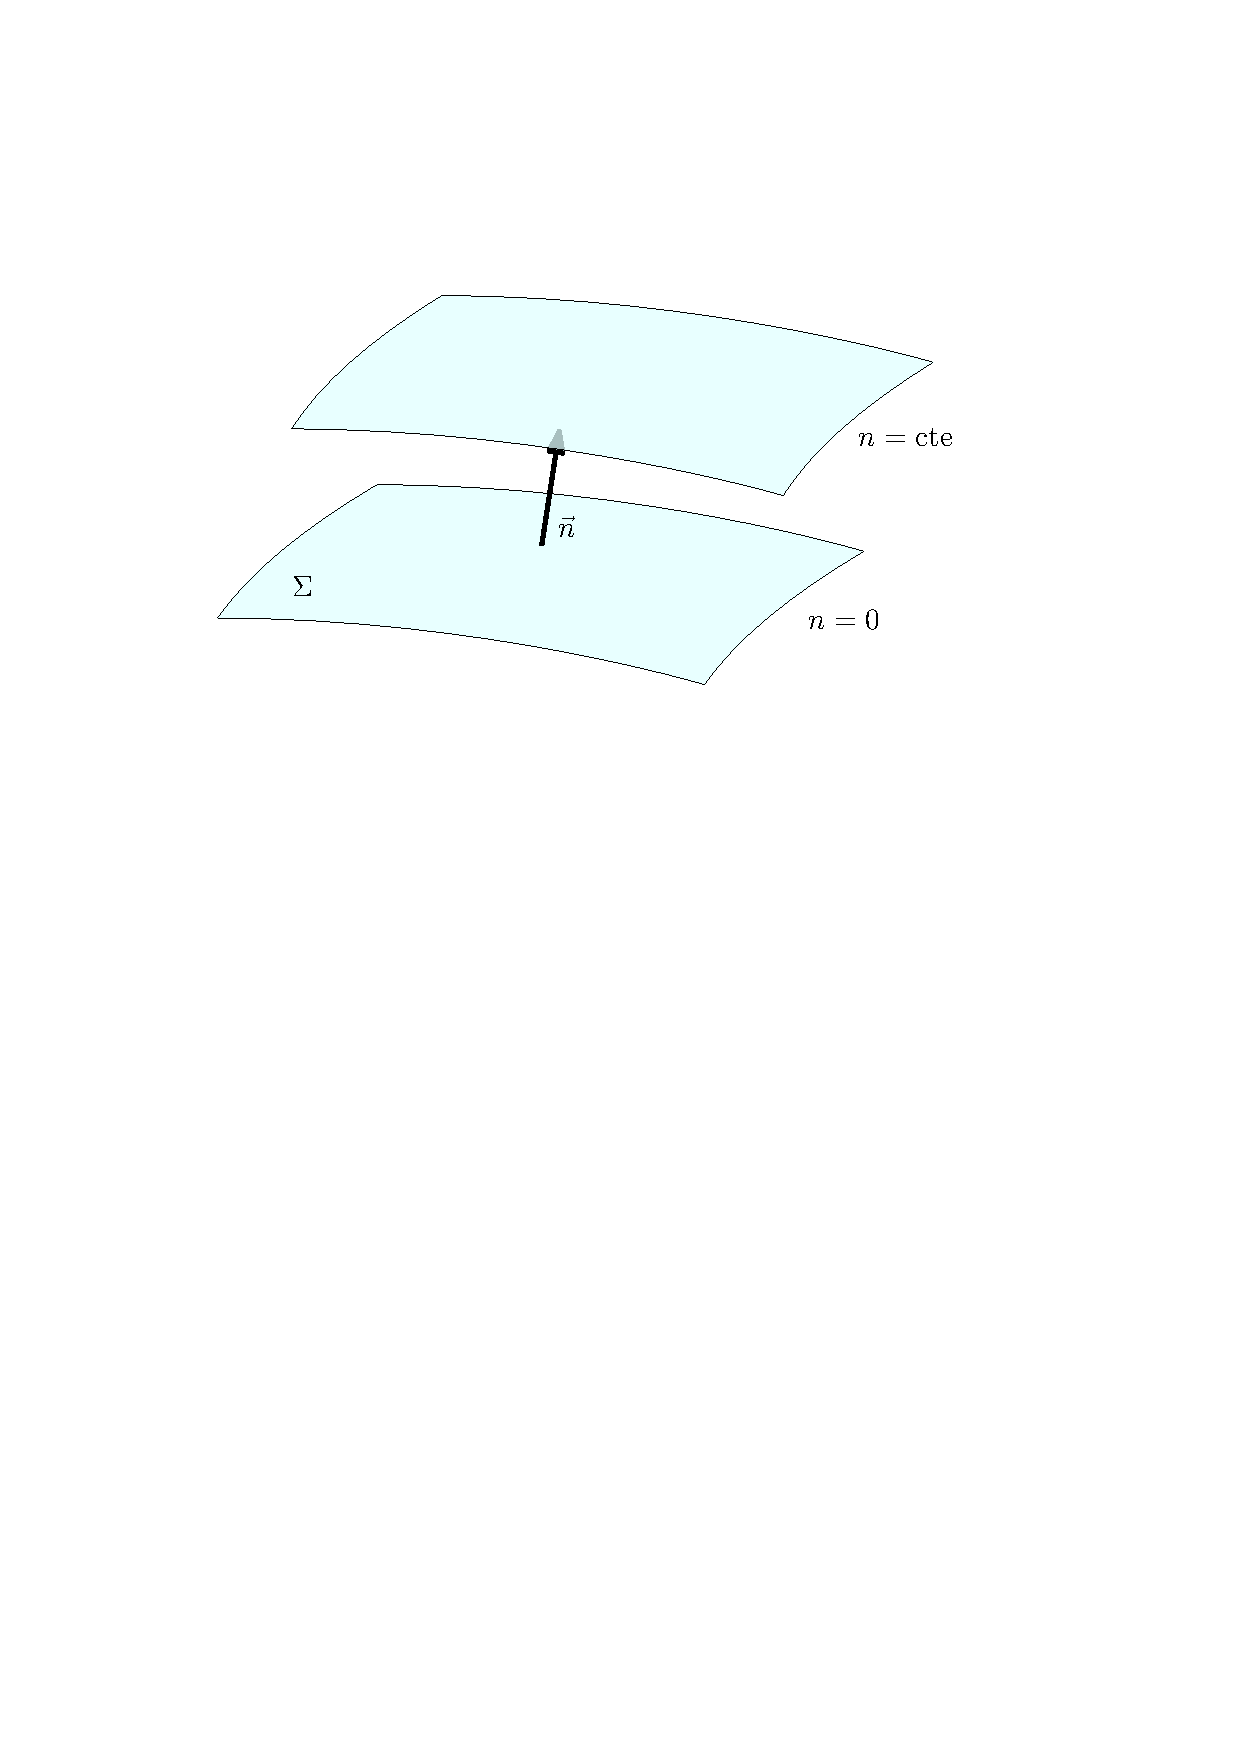
\includegraphics[width=0.7\linewidth]{figures/Junction.pdf}
     \caption{Coordenadas Gausianas en el vecindario a $\Sigma$}
     \label{JC}
 \end{figure}
Si a través de la superficie no hay contenido material, las condiciones de acoplamiento en estas coordenadas son:
 \begin{enumerate}[leftmargin=2cm]
     \item La métrica de las 3-superficies $g_{ij}$ es continua a través de $\Sigma$.
     \item El tensor de energía-momento superficial se anula
     \begin{equation}
\tensor{S}{^\alpha_\beta}\equiv\lim _{\varepsilon \rightarrow 0}\left[\int_{-e}^{+\varepsilon} T_{\beta}^{\alpha} d n\right]=0.
    \end{equation}
 \end{enumerate}

 Como es explicado en \cite{Misner1973} la condición 2 es equivalente a exigir la continuidad de la segunda forma fundamental. 
 
 \textbf{C2:} Para el caso considerado en este trabajo $\Sigma:\,r=R$, además la simetría esférica permite identificar $\vec{n}=\pdv{r}$ y debido a que la métrica exterior es la de Schwarzschild $\eval{T^{\alpha}_{\beta}}_{+\epsilon}$= 0, teniendo en cuenta estas consideraciones las condiciones de acoplamiento se reducen a
 \begin{enumerate}[leftmargin=2cm]
     \item $e ^ {  2 \nu(R) } =  1 - \frac { 2 M } { R }= e ^ { -2 \lambda(R) }$.
    \item $P(R)=\rho(R)=0$.
 \end{enumerate}


\subsection*{ Sobre el corrimiento al rojo gravitacional}
\noindent La luz emitida por una estrella es observada corrida al rojo por un observador lejano debido a la presencia del campo gravitacional. Qué tanto es corrida al rojo puede ser estimado de manera sencilla con u argumento basado en óptica geométrica \cite{Glendenning2000}: considerando un átomo de la estrella a una distancia $r$ de su centro, que emite un fotones con determinada frecuencia, el intervalo de tiempo propio entre dos emisiones consecutivas está dado por
\begin{equation}
d \tau=\sqrt{-g_{\mu \nu} d x^{\mu} d x^{\nu}},
\end{equation}
en el marco del átomo esto es simplemente ($dx^i=0$)
\begin{equation}
d \tau_{\mathrm{e}}=\sqrt{-g_{00}(r)} d t.
\end{equation}
El intervalo espacio-temporal para un rayo radial será
\begin{equation}
d \tau^{2}=g_{11}(r) d r^{2} - g_{00}(r) d t^{2} = 0,
\end{equation}
así que el tiempo que tardó un pulso en viajar de $r$ a $\infty$ es
\begin{equation}\label{timeinterval}
\Delta t=t_{\infty}-t_{r}= \int_{r}^{\infty}\left(\frac{g_{11}(\bar{r})}{g_{00}(\bar{r})}\right)^{1 / 2} d \bar{r}.
\end{equation}
Como $\Delta{t}$ no depende de $t$, el tiempo coordenado entre dos emisiones consecutivas $dt$, medido por un observador ubicado en $r$ es el mismo para el observador lejano. Con lo anterior en cuenta, el tiempo propio para el observador lejano será
\begin{equation}
d \tau_{\mathrm{o}}=\sqrt{-g_{00}(\infty)} d t.
\end{equation}
Como el inverso del tiempo propio es proporcional a la frecuencia, la razón entre la frecuencia emitida y observada es
\begin{equation}
\frac{\omega_{\mathrm{e}}}{\omega_{\mathrm{0}}}=\left(\frac{g_{00}(\infty)}{g_{00}(r)}\right)^{1 / 2}=e^{-\nu(r)},
\end{equation}
y con esto el corrimiento al rojo gravitacional es
\begin{equation}
    z(r)\equiv \frac{\omega_{\mathrm{e}}-\omega_{\mathrm{o}}}{\omega_{\mathrm{o}}}  = e^{-\nu(r)}-1.
    \label{redshift}
\end{equation}
Como luego se requerirá, la densidad de energía es una función que decrece desde centro del objeto compacto hasta la frontera. De manera consistente con esto, se espera que una señal de luz sea corrida al rojo en regiones con densidades de energía más altas y el corrimiento al rojo gravitacional debe ser también una función que decrece desde el centro hasta a la frontera.
\textbf{C3:} El corrimiento al rojo descrito por \eqref{redshift} debe disminuir con el incremento de $r$.
\subsection*{Sobre el signo de la densidad de energía y la presión}
\noindent Si bien la teoría cuántica de campos permite fenómenos de sub-vacío como la aparición de densidades de energía negativa locales \cite{Ford2010}, restricciones sobre magnitud y duración sugieren que es improbable que hayan consecuencias macroscópicas. Por esto se requiere que las densidades de energía sean positivas.
Así mismo, aunque los sistemas físicos pueden tener presiones negativas, esto solo ocurre en estados metaestables o de equilibrio parcial \cite{Landau1980}. Este tipo de estados tienen un determinado tiempo de relajación después del cual el sistema retorna a estados más estables. Por ende, como se estudiarán modelos estelares en equilibrio, se requiere la presión sea siempre positiva. 

\textbf{C4:} La densidad de energía y la presión deben ser positivas dentro de la estrella. 

\subsection*{Sobre la densidad de energía y la presión}

\noindent Una estrella Newtoniana modelada como un fluido perfecto es consistente con el principio de flotabilidad de Arquímedes: para que un elemento de fluido flote debe estar sobre fluido que sea más denso que él mismo, alcanzando un máximo en el centro. Como densidades altas implican presiones altas, el comportamiento de la presión es el mismo. Como en relatividad general los valores de la densidad de energía $\rho$ y la presión $P$ son locales, se espera que este comportamiento se mantenga.

\textbf{C5:} La densidad de energía y la presión deben alcanzar un máximo en el centro ($\rho'(0)=P'(0)=0$) y deben decrecer monótonamente hacia afuera.

\subsection*{Condiciones de energía}
\noindent Con el fin de obtener soluciones a las ecuaciones de Einstein en presencia de fuentes de energía y momento realistas es necesario imponer ciertas condiciones de energía que limiten la arbitrariedad del tensor energía-momentum escogido.

Existe una variedad de condiciones de energía que son usadas en diferentes circunstancias, las usadas con mayor frecuencia son \cite{Hawking1973,Carroll2003}:

\begin{itemize}[leftmargin=1.5cm]
    \item \emph{Condición de energía débil (WEC)}: el tensor de energía-momentum en cada punto $p$ de la variedad obedece la desigualdad $T_{\mu \nu} t^{\mu} t^{\nu} \geq 0$ para cualquier vector tipo tiempo $t^{\mu}\in T_{p}$.
    \item \emph{Condición de energía dominante (DEC)}: el tensor de energía-momentum en cada punto $p$ de la variedad obedece la desigualdad $T_{\mu \nu} t^{\mu} t^{\nu} \geq 0$ y además $T^{\mu \nu} t_{\mu}$ es un vector que no es tipo espacio para cualquier vector tipo tiempo $t^{\mu}\in T_{p}$.
    \item \emph{Condición de energía fuerte (SEC)}: el tensor de energía-momentum en cada punto $p$ de la variedad obedece la desigualdad $T_{\mu \nu} t^{\mu} t^{\nu} \geq \frac{1}{2} T_{\lambda}^{\lambda} t^{\sigma} t_{\sigma}$, para cualquier vector tipo tiempo $t^{\mu}\in T_{p}$.
\end{itemize}
Mientras que las condiciones débil y fuerte no se cumplen para el tensor energía-momento de algunos campos escalares con $m=0$ y $m\neq 0$ respectivamente \cite{Hawking1973}, la dominante es cumplida por todas las formas de materia conocidas y se requerirá por lo tanto que la materia en las estrellas de neutrones la cumpla. La DEC incluye a la WEC, como se verá esta prohíbe que los observadores midan densidades de energía negativas. La condición extra obliga a que la energía y el momento locales fluyan de pasado a futuro.

Escribiendo $t^\nu$ en una tétrada ortonormal $e_{\mu}$ como
\begin{equation}
    t^{\mu} e_{\mu}= \left(1+a^{2}+b^{2}+c^{2}\right)^{1 / 2} e_{0}+a e_{1}+b e_{2}+c e_{3},
\end{equation}
con el tensor de energía-momento de un fluido perfecto que se está considerando \eqref{EMT}, la condición $T_{\mu \nu} t^{\mu} t^{\nu} \geq 0$ se puede escribir como
\begin{equation}
T_{\mu \nu} v^{\mu} v^{\nu}=\left(1+a^{2}+b^{2}+c^{2}\right) \rho + \left( a^{2} +b^{2} +c^{2} \right) P \geq 0 \quad \forall a,b,c \in \mathbb{R},
\end{equation}
para el caso $a=b=c=0$ esto implica $\rho \geq 0$ y en el límite en que $a^2+b^2+c^2 \to \infty$ que $\rho + P \geq 0$.

Además, con $T^{\mu \nu} t_{\mu}$ escrito como
\begin{equation}
T^{\mu \nu} t_{\mu}e_{\nu}=\left(1+a^{2}+b^{2}+c^{2}\right)^{1 / 2} \rho e_{0}+a P e_{1}+b P e_{2}+c P e_{3},
\end{equation}
la condición de que no sea tipo espacio se convierte en
\begin{equation}
    -\rho^2 + (P^2-\rho^2)(a^2+b^2+c^2) \leq 0 \quad \forall a,b,c \in \mathbb{R},
\end{equation}
lo cual implica que $\rho \geq |P|$.

Debido a que en C1 se requirió que $\rho$ y $P$ fueran positivas, la condición de energía dominante añade la restricción $\rho \geq P$.

\textbf{C6:} La solución debe satisfacer la condición $\rho \geq P$.

\subsection*{Condición de causalidad}
\noindent El postulado de causalidad local en relatividad general prohíbe que una señal se propague a una velocidad mayor que la velocidad de la luz \cite{Hawking1973}. 

\textbf{C7:}  La velocidad del sonido en la estrella (modelada como un fluido perfecto) está dada por 
\begin{equation}
    v^2=\dv{P}{\rho},
\end{equation}
y esta no puede sobrepasar la velocidad de la luz:
\begin{equation}
    0 < \dv{P}{\rho} \leq 1 .
\end{equation}

\subsection*{Estabilidad ante pulsaciones radiales}

\noindent La teoría de oscilaciones radiales infinitesimales fue desarrollada por Chandrasekhar \cite{Chandrasekhar1964a}. En este enfoque se introduce un desplazamiento Lagrangiano (medido por un observador que se mueve con el fluido) $\xi(r,t)$ y se estudia su evolución dinámica de acuerdo a las ecuaciones de Einstein, la conservación local de la energía-momento y las leyes de la termodinámica, todas propiamente linealizadas.

Se puede demostrar \cite{Chandrasekhar1964a,Misner1973} que al suponer un desplazamiento con una dependencia temporal sinusoidal $\xi(r, t)=\mathrm{e}^{-\mathrm{i} \omega t} \zeta(r)$  y condiciones de frontera apropiadas, la ecuación que gobierna la dinámica de las perturbaciones radiales se convierte en un problema de autovalores para la frecuencia del desplazamiento $\omega$. La condición de estabilidad en este esquema se reduce al requerimiento $\omega \geq 0$, ya que para $\omega<0$ el desplazamiento $\xi(r,t)$ crece exponencialmente con el tiempo.   

Los diferentes criterios de estabilidad ante pulsaciones radiales se diferencian en la función de prueba $\zeta$ escogida y las aproximaciones que se hagan para obtener condiciones simples que aseguren $\omega \geq 0$.


\subsection*{Criterio de estabilidad del índice adiabático }

\noindent Chandrasekhar aplicó el formalismo para mostrar que las condiciones suficientes para la estabilidad dinámica (de distribuciones esféricas de materia) son más restrictivas en relatividad general que en la teoría Newtoniana. Como ejemplo, se puede comparar el límite inferior Newtoniano para el índice adiabático, necesario para asegurar la  estabilidad
\begin{equation}
    \gamma \equiv \frac { \rho + P  } { P } \dv{P}{\rho} \geq \frac{4}{3},
\end{equation}
con lo obtenido en relatividad general para una esfera de densidad e índice adiabático constantes
\begin{equation}
    \gamma \geq \frac{4}{3} +  \frac{19}{42} \frac{2M}{R}.
\end{equation}

Una condición más realista para asegurar la estabilidad, la cual toma en cuenta que el índice adiabático depende de la coordenada $r$, fue formulada por Merafina y Ruffini \cite{Merafina1989} en términos de un índice adiabático efectivo $\langle\gamma\rangle$ definido como

\begin{equation}
    \langle\gamma\rangle\equiv\frac{\int_{0}^{R} e^{\lambda+3 \nu} \gamma(r) P(r) r^{2} d r}{\int_{0}^{R} e^{\lambda+3 \nu} P(r) r^{2} d r}.
\end{equation}

\textbf{C8:} El índice adiabático efectivo debe satisfacer
\begin{equation}
     \langle\gamma\rangle \geq \gamma_{cr},
\end{equation}
donde $\gamma_{cr}$ está dado por
\begin{align}\label{gammacrit}
    \gamma_{cr} = \frac{4}{3} +& \frac{1}{36} \frac{\int_{0}^{R} e^{\lambda+3 \mathrm{v}}\left[16 P+\left(e^{\lambda}-1\right)\left(P+\rho \right)\right]\left(e^{\lambda}-1\right) r^{2} d r}{\int_{0}^{R} e^{\lambda+3 \mathrm{v}} P r^{2} d r} \nonumber
    \\ &+ \frac{4 \pi}{9} \frac{\int_{0}^{R} e^{3( \lambda+ \mathrm{v})}\left[8 P+\left(e^{\lambda}+1\right)\left(P+\rho \right)\right] P r^{4} d r}{\int_{0}^{R} e^{\lambda+3 \mathrm{v}} P r^{2} d r}
    \\ & + \frac{16 \pi^{2} }{9} \frac{\int_{0}^{R} e^{5 \lambda+3 v }\left(P+\rho \right) P^{2} r^{6} d r}{\int_{0}^{R} e^{\lambda+3 v } P r^{2} d r}. \nonumber
\end{align}

\cmmt{
\begin{align}
\begin{aligned} \gamma_{c r} &=\left[-4 \int_{0}^{R} e^{(\lambda+3 \nu) / 2} r^{3} \frac{d P}{d r} d r+\int_{0}^{R} e^{(\lambda+3 \nu) / 2}\left(\frac{d P}{d r}\right)^{2} \frac{r^{4}}{P+\rho} d r\right.\\ &\left.-\frac{8 \pi G}{c^{4}} \int_{0}^{R} e^{3(\lambda+\nu) / 2} P (P+\rho) r^{4} d r\right] \times\left(9 \int_{0}^{R} e^{(\lambda+3 \nu) / 2} P r^{2} d r\right)^{-1} \end{aligned}
\end{align}
}
\subsection*{Criterio de Harrison-Zeldovich-Novikov}

\noindent La condición C8 es una condición suficiente para la estabilidad ante pulsaciones radiales. Zel'dovich \& Novikov \cite{Zeldovich1971} y Harrison, et al. \cite{Harrison1965} formularon una condición de estabilidad necesaria que es más fácil de aplicar. Usando diferentes argumentos, identificaron que para un modo normal y EOS dados, la frecuencia de las pulsaciones $\omega$ pasa de ser positiva a negativa en el mismo valor de la densidad central $\rho_c$ para el cual se alcanza la masa máxima $M_{\text{max}}$. 

Así que una manera sencilla de identificar modelos que sean inestables es usar el diagrama $M(\rho_c)$ para identificar el valor de $\rho_c$ para el cual se alcanza el máximo, los modelos con $\rho_c$ mayor serán inestables. 

\textbf{C10:} Para una configuración sea estable respecto a oscilaciones radiales es \emph{necesario} que su masa $M$ aumente a medida que la densidad central $\rho_{c}$ crece: 

\begin{equation}
    \frac { \partial M \left( \rho _ { c } \right) } { \partial \rho _ { c } } > 0.
\end{equation}
Además, los puntos en los que $\frac { \partial M \left( \rho _ { c } \right) } { \partial \rho _ { c } } = 0$ (puntos críticos) son puntos donde la configuración pasa de estabilidad a inestabilidad.



\subsection*{Estabilidad ante cracking}
\noindent El cracking es una posible inestabilidad de esferas anisótropas ($P_r \neq P_{\perp}$) ante perturbaciones locales de densidad. Cuando estas perturbaciones son constantes, se puede demostrar \cite{Abreu2007} que las configuraciones estables ante cracking deben satisfacer
\begin{equation}\label{abreucracking}
    -1 \leq v_{s \perp}^{2}-v_{s r}^{2} \leq 0.
\end{equation}
Además, como fue demostrado por \cite{Ivanov2017} \eqref{abreucracking} es equivalente al requerimiento
\begin{equation}
    0 \geq \frac{\mathrm{d} P_{\perp}}{\mathrm{d} r} \geq \frac{\mathrm{d} P}{\mathrm{d} r}.
\end{equation}
Para modelos isótropos ($P_r=P_{\perp}=P$), esto se reduce a 
\begin{equation}
    0 \geq \frac{\mathrm{d} P}{\mathrm{d} r},
\end{equation}
esta condición asegura que la presión decrece monótonamente y por lo tanto concuerda con la condición C5.

\textbf{C9:} El criterio para que una distribución sea estable ante cracking, en el caso de perturbaciones de densidad constantes, es 
\begin{equation}
    \dv{P}{r} \leq 0.
\end{equation}


\subsection*{Estabilidad ante convección adiabática}

\noindent La estabilidad contra convección se puede entender como sigue: cuando un elemento de fluido es desplazado rápidamente hacia abajo, si su densidad aumenta más rápido que la densidad que lo rodea, el elemento se hundirá y la configuración será inestable. Por otro lado, si la densidad del elemento de fluido es menor que la de su alrededor, este flotará y la estrella será estable ante convección \cite{Bondi1964a}. 

Hernández et al. derivaron en \cite{Hernandez2018} una condición sencilla que asegura estabilidad ante la convección adiabática. Siguiendo su trabajo: si se denota a $\rho(r_p)$ como la densidad de un elemento de fluido en su posición original $r_p$ y se desplaza el elemento hacia abajo, se tiene
\begin{equation}
    \rho\left(r_{p}\right) \rightarrow \rho\left(r_{p}\right)+\delta \rho(r),\quad \text {con } \quad \delta \rho(r)=\rho^{\prime}(r)(-\delta r) \quad \text { y } \quad r=r_{p}-\delta r,
\end{equation}
donde $r$ es la nueva posición del elemento de fluido y $-\delta r$ el desplazamiento hacia el centro. 
Como $\rho^{\prime} < 0$, $\delta \rho(r)$ es positivo y la densidad del elemento de fluido que fue comprimido será mayor en $r$ que en $r_p$. 
Expandiendo la densidad del ambiente en $r$ a primer orden en $-\delta r$ se obtiene
\begin{equation}
    \rho\left(r_{p}-\delta r\right) \approx \rho\left(r_{p}\right)+\rho^{\prime}\left(r_{p}\right)(-\delta r).
\end{equation}
Según lo ya explicado, el sistema será estable si la densidad del ambiente es mayor o igual a la densidad del elemento de fluido:
\begin{align*}
    \rho\left(r_{p}\right)+\rho^{\prime}\left(r_{p}\right)(-\delta r) &\geq \rho\left(r_{p}\right)+\rho^{\prime}(r)(-\delta r) \\ \rho^{\prime}\left(r_{p}\right) &\leq \rho^{\prime}(r).
\end{align*}
Expandiendo ahora $\rho^{\prime}(r)$ alrededor $r_p$ se obtiene
\begin{equation}
    \rho^{\prime}\left(r_{p}\right)+\rho^{\prime \prime}\left(r_{p}\right) \delta r \leq \rho^{\prime}\left(r_{p}\right),
\end{equation}
de donde se obtiene el criterio de estabilidad ante convección adiabática
\begin{equation}
    \rho^{\prime \prime}(r) \leq 0.
\end{equation}

En principio parece que este criterio es válido solo para perturbaciones muy rápidas: así asegura que la escala de tiempo hidrodinámica $\tau_h$ sea menor a la escala de tiempo térmica $\tau_t$ y se puede ignorar el transporte de calor. Sin embargo, es sabido que $\tau_h \ll \tau_t$ durante todas las fases de evolución estelar \cite{Bisnovatyi-Kogan2011}, por lo que el criterio es válido en situaciones más generales.  

\textbf{C11:} Para que un modelo estelar sea estable ante movimientos convectivos adiabáticos, el perfil de densidad $\rho(r)$ debe cumplir: 
\begin{equation}
    \rho ^ { \prime \prime } ( r ) \leq 0.
\end{equation}
\chapter{Solución numérica de las ecuaciones de TOV}\label{NumSol}
\noindent En este capítulo se discutirá el esquema numérico utilizado para solucionar las ecuaciones de TOV y se verificará la confiabilidad de éste comparando sus resultados con algunas de las soluciones interiores exactas conocidas.
La implementación en Python de la información presente en este apéndice se encuentra en el notebook de Jupyter Static Structure Manual\footnote{\url{https://nbviewer.jupyter.org/github/DavidRamosSal/stellar_structure/blob/master/Static_structure_manual.ipynb}}.

\section{Escalamiento del sistema de ecuaciones}
\noindent Las ecuaciones de TOV en unidades gravitacionales son
\begin{align}
    \frac{dm}{dr}=&4\pi \rho r^2 ,\\
    \frac{dP}{dr}=&-(\rho+P)\frac{m+4\pi r^3 P}{r(r-2m)} , \\
    \frac{d\nu}{dr}=& \frac{m+4\pi r^3 P}{r(r-2m)} =  -\frac{1}{\rho+P}\frac{dP}{dr},
\end{align}
sujetas a una ligadura dada por la ecuación de estado $P=P(\rho)$ y valores iniciales $\rho(r=0)=\rho_c$, $m(r=0)=0$ y $\nu(r=0)=\text{cte}$.

Debido a que los valores de las cantidades físicas cambian en varios órdenes de magnitud a lo largo de la extensión de la estrella, es necesario/preferible/útil re-escalar todas las variables dimensionales usando una constante con las mismas dimensiones conocida como la 'escala', esto con el doble propósito de convertir las variables en variables adimensionales y hacer su valor alrededor de la unidad \cite{Langtangen2016}.

Re-escalando las variables como
\begin{equation}
    \rho=\rho_* \bar{\rho} \quad ; \quad P=P_* \bar{P} \quad ; \quad m=m_*\bar{m} \quad ; \quad r=r_*\bar{r},
\end{equation}
el sistema de ecuaciones se convierte en
\begin{align}
\frac{d\bar{m}}{\bar{dr}}=&\left( \frac{\rho_* r_*^3}{m_*} \right) 4\pi \bar{\rho} \bar{r}^2 ,\\
\frac{d\bar{P}}{d\bar{r}}=&-\left( \frac{m_*}{r_* \rho_*} \right)\left(\frac{\rho_*}{P_*}\bar{\rho}+\bar{P}\right)\frac{\bar{m}+\left( \frac{r_*^3 P_*}{m_*} \right)4\pi \bar{r}^3 \bar{P}}{\bar{r}\left(\bar{r}-\frac{m_*}{r_*}2\bar{m}\right)} , \\
 \frac{d\nu}{d\bar{r}}=&-\frac{1}{\left(\bar{P}+\frac{\rho_*}{P_*}\bar{\rho}\right)}\frac{d\bar{P}}{d\bar{r}}.
\end{align}
Escogiendo la escala de $m$, $P$ y $\nu$ de modo que el sistema de ecuaciones adimensionales mantenga la forma del sistema original se obtienen las relaciones
\begin{equation}
    P_*=\rho_*,\quad r_*=\frac{1}{\sqrt{\rho_*}} ,\quad m_*=r_* ,
\end{equation}
así que se pueden escribir todas las constantes de escalamiento en términos de una sola.
Escogiendo $\rho_*$ como la constante independiente, el último paso consiste en usar un valor que refleje la escala de densidades del problema. A partir de la masa del neutrón $m_n$, se puede construir una densidad $\rho_* = \frac{m_{n}^{4}c^{3}}{8 \pi^2 \hbar^3}\sim 2\times 10^{15}\,\text{g/cm}^{3}$ como un valor característico de las densidades centrales de las estrellas de neutrones.

El sistema re-escalado a solucionar será
\begin{align}\label{adimensional}
      \frac{d\bar{m}}{d\bar{r}}=&4\pi \bar{\rho} \bar{r}^2 , \nonumber \\
    \frac{d\bar{P}}{d\bar{r}}=&-(\bar{\rho}+\bar{P})\frac{\bar{m}+4\pi \bar{r}^3 \bar{P}}{\bar{r}(\bar{r}-2\bar{m})} , \\
    \frac{d\bar{\nu}}{d\bar{r}}=& \frac{\bar{m}+4\pi \bar{r}^3 \bar{P}}{\bar{r}(\bar{r}-2\bar{m})} =  -\frac{1}{\bar{\rho}+\bar{P}}\frac{d\bar{P}}{d\bar{r}},\nonumber
\end{align}
con la ecuación de estado expresada en términos de las variables adimensionales $\bar{P}=\bar{P}(\bar{\rho})$ y los valores iniciales $\bar{\rho}(\bar{r}=0)=\rho_c / \rho_{*}$, $\bar{m}(\bar{r}=0)=0$ y $\bar{\nu}(\bar{r}=0)=\text{cte}$.

\section{Integración del sistema}

\noindent La integración numérica del sistema de ecuaciones diferenciales ordinarias \eqref{adimensional} se realizó usando el método de Runge-Kutta de cuarto orden, donde el paso de integración se escogió como una fracción $\delta$ de una escala de distancias definida a partir de los gradientes de presión y masa \cite{Baym1971}: 
\begin{equation}\label{adaptivestep}
    \Delta{r} = \delta \left( \frac { 1 } { m } \frac { \mathop{dm} } { \mathop{dr}  } - \frac { 1 } { P } \frac { \mathop{dP}  } { \mathop{dr} } \right) ^ { - 1 }.
\end{equation}

Haciendo uso de este paso adaptativo se evade la necesidad de tener un estimado del radio de la estrella al determinar un valor sensible para el paso fijo, pues $\Delta$ disminuye cuando $m$ o $P$ cambian rápidamente. Sólo es necesario escoger un paso inicial pequeño para evitar la singularidad del paso en $r=0$.

La singularidad del gradiente de $\bar{P}$ en $r=0$ puede evitarse expandiendo $\bar{\rho}$ como una función de $\bar{r}$ en la ecuación del gradiente de $\bar{m}$
\begin{equation*}
    \frac{d\bar{m}}{\bar{dr}}=4\pi \bar{r}^2 \left(  \bar{\rho} _ { c } + \left. \frac { \partial \bar{\rho }} { \partial \bar{r} } \right| _ { \bar{r} = 0 } \bar{r} + \ldots \right),
\end{equation*}
manteniendo sólo el término constante e integrando se obtiene
\begin{equation*}
    \bar{m}  =  \frac { 4 } { 3 } \pi \bar{r} ^ { 3 } \bar{\rho} _ { c },
\end{equation*}
con lo que el gradiente de $\bar{P}$ cerca $\bar{r}=0$ se puede escribir como
\begin{equation}
    \frac{d\bar{P}}{d\bar{r}} = -4\pi (\bar{P}+\bar{\rho}_c)\frac{\left(\frac{\bar{\rho}_c}{3}+\bar{P}\right)}{1-\frac{8}{3}\pi\bar{r}^2\bar{\rho}_c} \bar{r},
\end{equation}
esta aproximación es válida mientras $ \frac{\bar{\rho}}{\bar{\rho}_{c}} \sim 1$.

Debido a que las ecuaciones de estado consideradas se encuentran tabuladas solo para ciertos valores de $\rho$ y $P$, estas deben ser interpolada para los valores intermedios requeridos en cada paso de integración. Esto se realizó interpolando linealmente $\log{\rho}$ como una función de $\log{P}$ (lo cual es una práctica común \cite{Haensel2007}).

\section{Comparando con soluciones exactas}

\noindent Para verificar que los resultados obtenidos usando la rutina numérica creada son confiables, estos pueden ser comparados soluciones exactas a las ecuaciones de TOV que se obtienen al imponer ciertas relaciones entre las variables físicas o una ecuación de estado lo suficientemente simple. 

A continuación se presentará solamente la comparación con la solución Tolman VII \cite{Tolman1939}, pues es una de las soluciones exactas de mayor interés por su posibilidad de modelar configuraciones estelares realistas \cite{Negi2004}. Comparaciones con otras soluciones exactas pueden ser encontradas en el Notebook de Jupyter.    

Tomando una muestra de 200 puntos de los perfiles de densidad y presión correspondientes a la solución Tolman VII para algún valor de la compacidad $\mu$, se obtiene un conjunto de valores ($r_i, \rho_i, P_i$) que si se ignorar la coordenada $r$ puede ser usada como la EOS correspondiente a la solución exacta. Usando esta EOS para resolver las ecuaciones de TOV con la rutina numérica construida, de acuerdo a lo expuesto en la sección anterior, se puede apreciar que las dos soluciones concuerdan muy bien (ver Figura \ref{Exact}). 

\begin{figure}%[H]
    \centering
    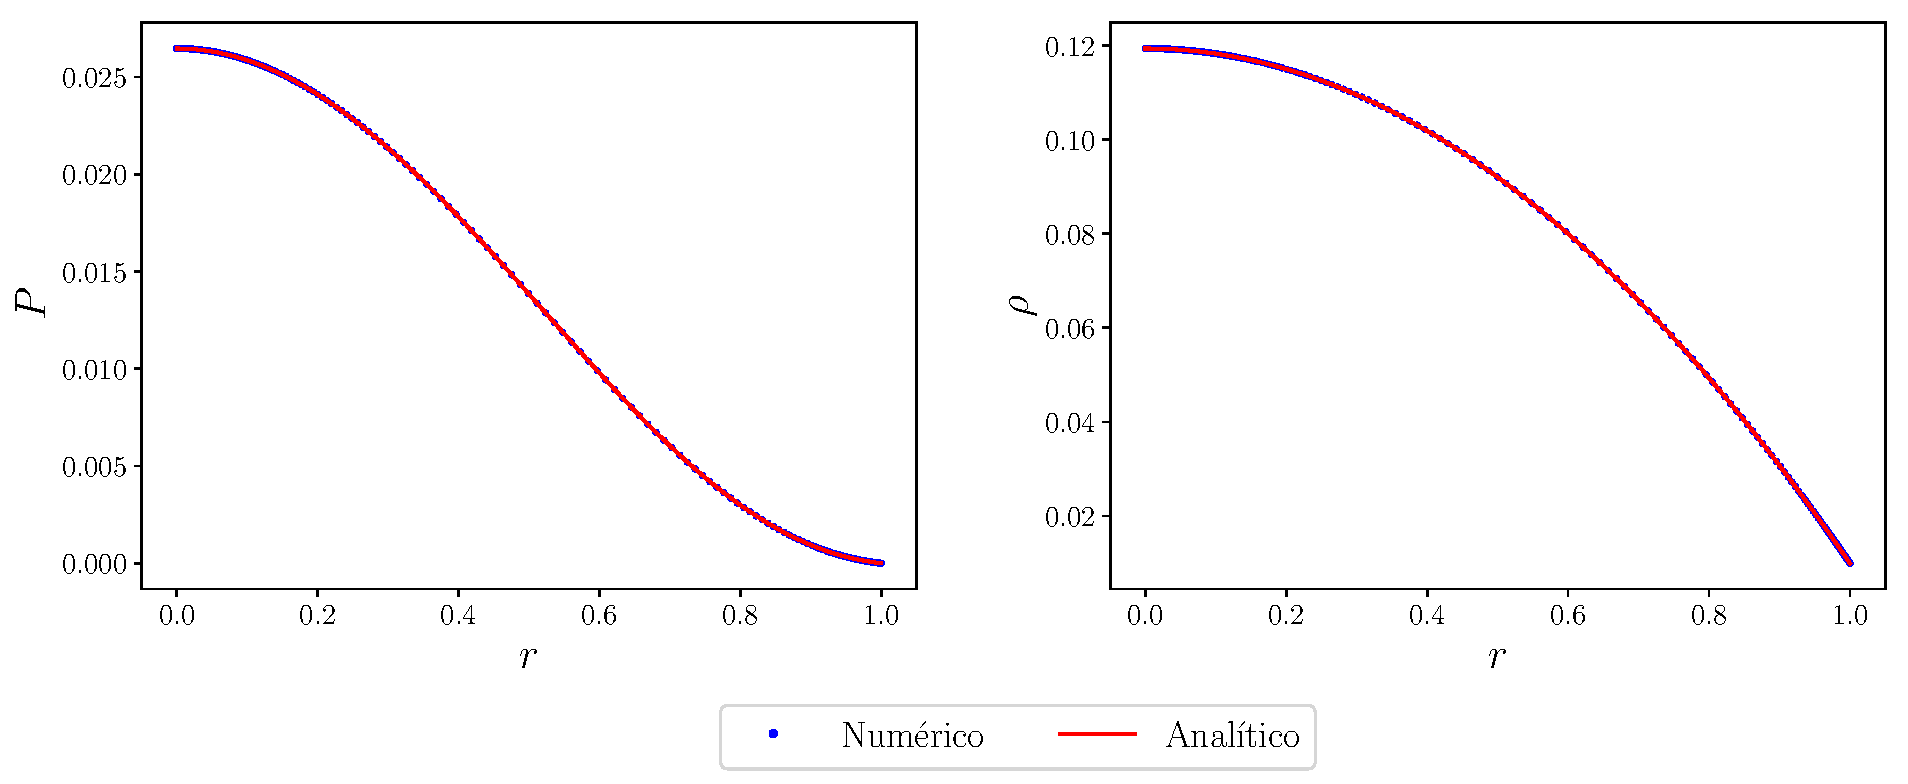
\includegraphics[width=\linewidth]{figures/ProfilesTolmanVIImu45.pdf}
    \caption[Comparación entre una solución exacta y su análogo numérico]{Comparación entre los perfiles de presión y densidad numéricos y analíticos para una compacidad $\mu=0.45$.}
    \label{Exact}
\end{figure}

La convergencia del paso adaptativo usado \eqref{adaptivestep} se puede verificar hallando el error entre la solución exacta y la numérica para distintos valores de $\delta$ ya que $\delta$ maneja la cantidad de pasos que se tomarán por caída de masa y presión (ver Figura \ref{ErrorExact}). 

\begin{figure}%[H]
    \centering
    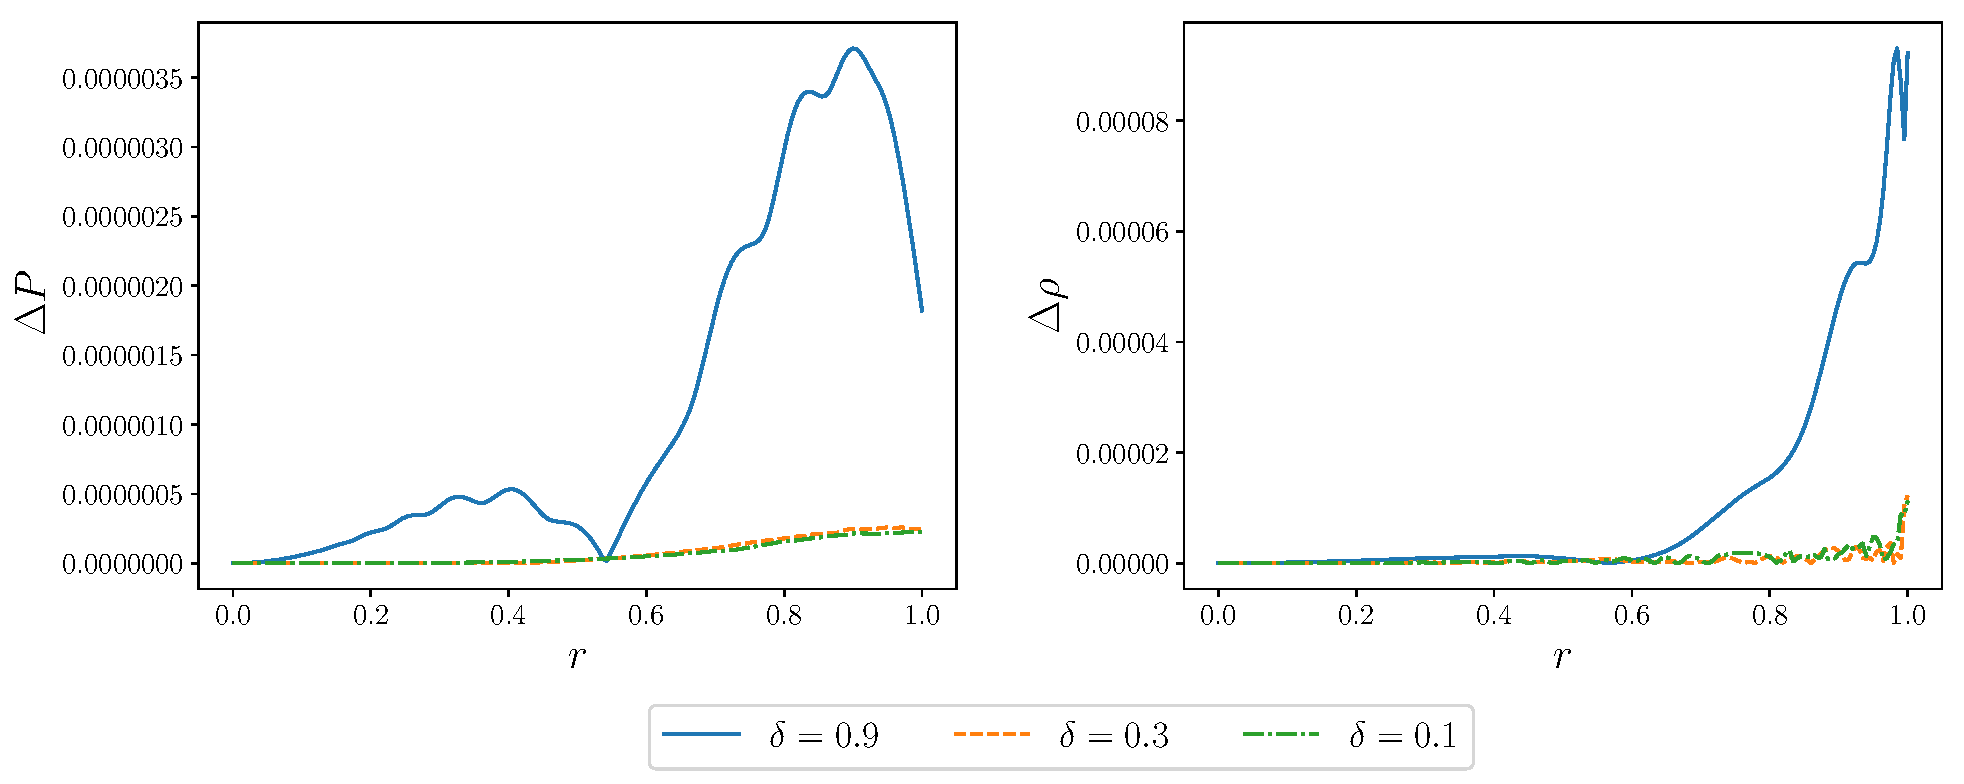
\includegraphics[width=\linewidth]{figures/ErrorTolmanVIImu45.pdf}
    \caption[Error de la solución numérica respecto a la exacta]{Error de la solución numérica como función de $r$ para distintos valores de $\delta$. Para $\delta=0.9$ se obtuvo los errores más grandes, como era de esperarse y converge rápidamente: la diferencia entre usar $\delta=0.3$ y $\delta=0.1$ no es significante.}
    \label{ErrorExact}
\end{figure}


\section{Derivadas numéricas de las variables físicas}\label{NumDer}  

\noindent Para evaluar algunas de las condiciones de aceptabilidad fue necesario hallar derivadas numéricas de un arreglo con respecto a otro. Esto en principio se puede realizar fácilmente usando diferencias finitas, sin embargo la presencia de discontinuidades propias de las EOS y de su interpolación hacen que sea poco práctico usarlas. La alternativa que se encontró fue satisfactoria fue interpolar los arreglos a derivar usando un spline suavizado y hallar la derivada del spline. La librería de Python Scipy\footnote{\url{https://www.scipy.org}} cuenta con una rutina llamada UnivariateSpline\footnote{\url{https://docs.scipy.org/doc/scipy-0.17.0/reference/generated/scipy.interpolate.UnivariateSpline.html}} que permite realizar la interpolación y hallar su derivada fácilmente.
\begin{figure}[H]
    \centering
    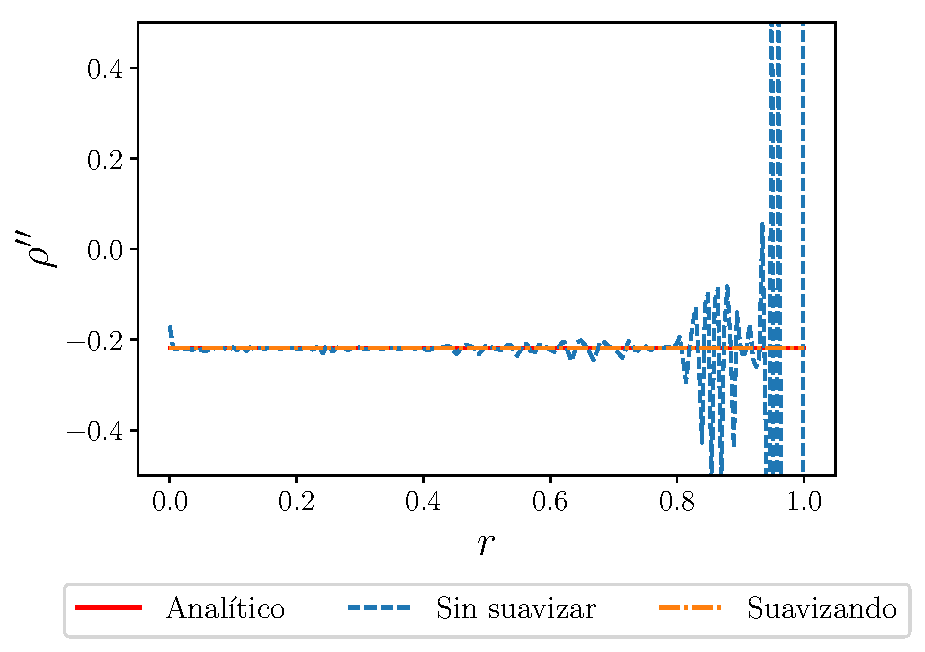
\includegraphics[width=0.7\linewidth]{figures/rhoppTolmanVIImu45.pdf}
    \caption[Comparación entre $\rho^{\prime\prime}$ para una solución exacta y lo obtenido numéricamente]{Comparación de la segunda derivada del perfil de densidad con respecto a $r$ analítica, numérica sin suavizar y suavizada con un factor de suavizamiento de $10^{-5}$, para la solución exacta Tolman VII con $\mu=0.45$. Se aprecia cómo un pequeño factor de suavizamiento es suficiente para obtener una derivada numérica precisa. }
    \label{numericald}
\end{figure}
Como un ejemplo de cómo el hecho de que el spline sea suavizado ayuda a mejorar la derivación numérica, se usó la segunda derivada con respecto a $r$ del perfil de densidad de la solución exacta presentada en la sección anterior y se halló la misma derivada al perfil numérico con la rutina mencionada (ver Figura \ref{numericald}). 
Se puede observar cómo la derivada del spline sin suavizar presenta grandes oscilaciones, que indican un \quotes{overfitting}. Por otro lado al usar un pequeño factor de suavizamiento la cantidad de nodos que se utilizan se reduce y las dos derivadas coinciden.

\chapter{Resultados}

\noindent Las ecuaciones de TOV \eqref{dmtov},\eqref{dptov} y \eqref{dnutov} fueron resueltas para un amplio rango de densidades centrales. Con esto, las condiciones C1-C11 presentadas en la Sección \ref{phyacep} pueden ser evaluadas, con el fin de determinar si los modelos de estrellas de neutrones obtenidos con las ecuaciones de estado disponibles en la literatura son físicamente viables.

De las 11 condiciones de aceptabilidad, las condiciones C1-C5 son consistentes con las ecuaciones de TOV y la construcción del la rutina numérica, y por lo tanto no serán verificadas. De las condiciones restantes, la condición de estabilidad ante cracking C9 no se exploró en este trabajo. Teniendo lo anterior en cuenta, las condiciones de aceptabilidad física con las que se evaluarán los modelos son C6, C7, C8, C10 y C11.

%Con el fin de determinar si los modelos de estrellas de neutrones obtenidos con las ecuaciones de estado de la materia densa disponibles en la literatura son físicamente viables, se resolvieron las ecuaciones de TOV \eqref{dmtov},\eqref{dptov} y \eqref{dnutov} para un amplio rango de densidades centrales y se evaluaron las condiciones C1-C11 presentadas en la Sección \ref{phyacep}.

En la siguiente sección se describirá detalladamente el proceso de verificación de las condiciones para la EOS ENG \cite{Engvik1994}. Esta EOS fue elegida porque predice una masa máxima $M_{\text{max}}= 2.241 > 2.14M_{\odot}$, la masa más alta medida a la fecha, correspondiente al pulsar MSP J0740+6620 \cite{Cromartie2019}. Este valor para $M_{\text{max}}$ satisface además los límites más conservadores impuestos por la primera observación de ondas gravitacionales por la fusión de dos estrellas de neutrones GW170817 y su contraparte electromagnética \cite{Rezzolla2017,Radice2018,Ruiz2018,Shibata2019}. Después se presentarán los resultados consolidados para un conjunto 37 EOSs realistas (incluyendo ENG) basados en la elección de EOSs presentada en la revisión \cite{Ozel2016}.

\section{Un caso particular: la ecuación de estado ENG}

\noindent La ecuación de estado ENG considera material compuesto de neutrones, protones, electrones y muones. El problema de muchos cuerpos es abordado usando un enfoque miscroscópico basado en el método de Dirac-Brueckener-Hartree-Fock.  

Los requisitos mínimos de consistencia física que una ecuación de estado debe cumplir son la condición de energía dominante (C6) y la condición de causalidad (C7). Estas condiciones dependen enteramente de la construcción de la ecuación de estado y pueden ser verificadas sin necesidad de resolver las ecuaciones de TOV. En las Figuras \ref{DECeng} y \ref{SSCeng} se verificó que la EOS ENG cumple las condiciones C6 y C7.

Tras confirmar que la ecuación de estado cumple C6 y C7, se procede a solucionar las ecuaciones de TOV para un conjunto de densidades centrales (valores iniciales) que típicamente va desde $\rho_c=\rho_0 \sim 10^{14} \text{g cm}^{-3}$ hasta la máxima densidad disponible en la ecuación de estado. Como por construcción las soluciones cumplen las condiciones C1, C2, C3, C4 y C5 , se utiliza la condición C10 para restringir los modelos a analizar: sólo se considerarán modelos con densidades centrales tales que $\frac { \partial M \left( \rho _ { c } \right) } { \partial \rho _ { c } } > 0$. Esta derivada es nula para la configuración con masa máxima y se presenta un cambio del signo de la derivada de positiva a negativa, la densidad central para la que esto sucede indica el inicio de las configuraciones inestables (ver Figura \ref{mrhoeng}).

\begin{figure}[H]
   \begin{minipage}[b]{.48\textwidth}
        \centering
        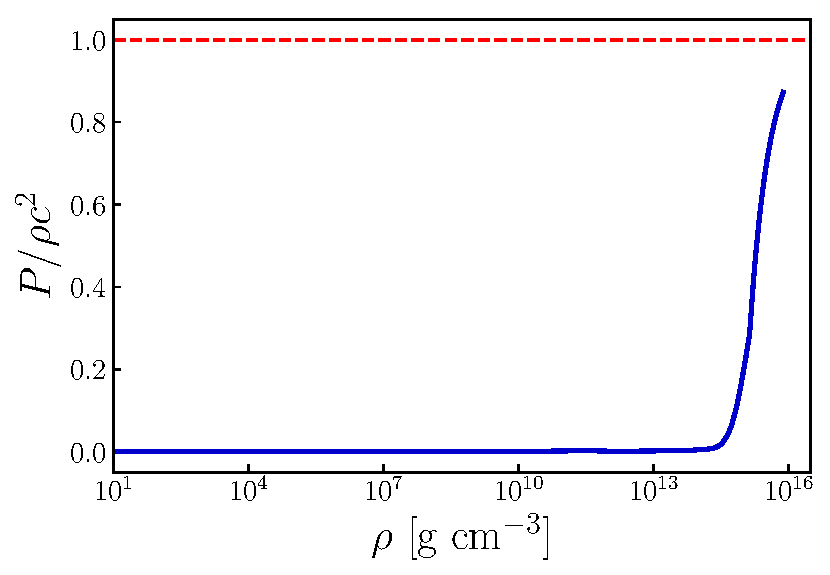
\includegraphics[width=1\textwidth]{figures/ECeng.pdf}
        \caption[Verificación de C6 para la EOS ENG]{Verificación de C6 para la EOS ENG. La línea roja punteada indica la igualdad $P=\rho c^2$. Se aprecia que $P/\rho c^2 \leq 1$, por lo que esta ecuación de estado cumple C6.}
        \label{DECeng}
    \end{minipage}
    \quad
    \begin{minipage}[b]{.48\textwidth}
        \centering
        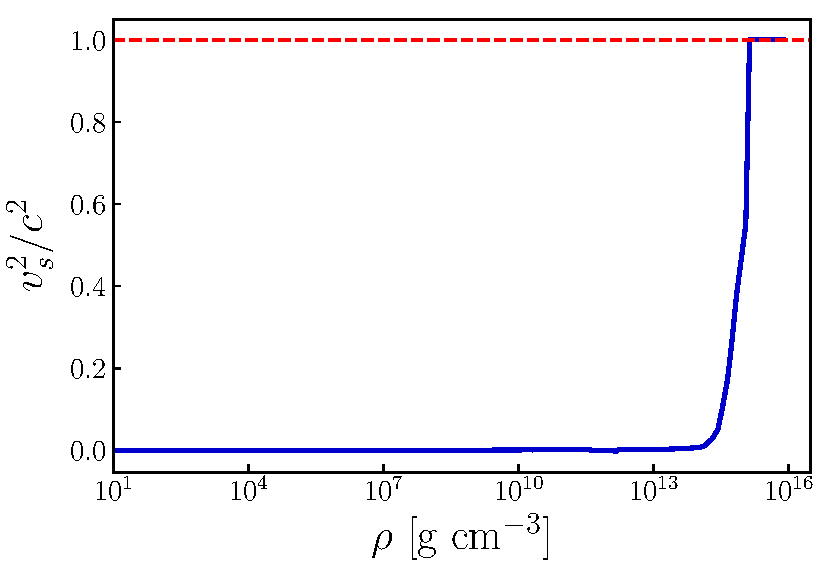
\includegraphics[width=1\textwidth]{figures/SSeng.pdf}
        \caption[Verificación de C7 para la EOS ENG]{Verificación de C7 para la EOS ENG. La línea roja punteada representa $v_s=c$. Se aprecia que $v_s^2/c^2 \leq 1$, por lo que esta ecuación de estado cumple C7.}
        \label{SSCeng}
    \end{minipage}
\end{figure}



\begin{figure}[H]
    \centering
    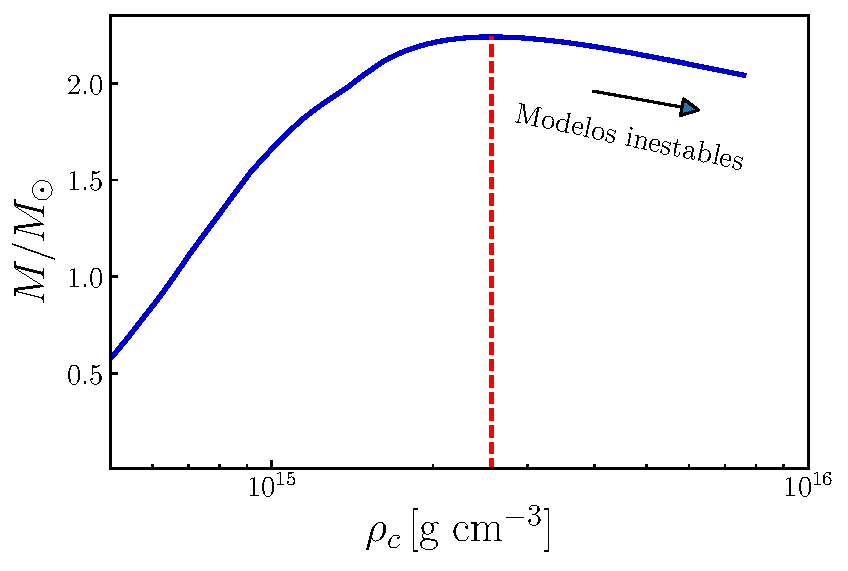
\includegraphics[width=0.7\linewidth]{figures/Mrhorel_eng.pdf}
    \caption[Identificando los modelos obtenidos con la EOS ENG que no satisfacen C10]{Identificando los modelos obtenidos con la EOS ENG que no satisfacen C10. La masa máxima para esta ecuación de estado fue $M_{max}=2.241\,M_{\odot}$ alcanzada con la densidad central $\rho_c=2.5704 \times 10^{15}$ (línea roja punteada), así que modelos con $\rho_c \geq 2.5704 \times 10^{15}$ serán inestables ante pulsaciones radiales. }
    \label{mrhoeng}
\end{figure}
%Tras confirmar que la ecuación de estado cumple C6 y C7, se procede a solucionar las ecuaciones de TOV para un conjunto de densidades centrales (valores iniciales) que típicamente va desde $\rho_c=\rho_0 \sim 10^{14} \text{g cm}^{-3}$ hasta la máxima densidad disponible en la ecuación de estado. Como por construcción las soluciones cumplen las condiciones C1,C2,C4 y C5 (como es descrito en el Apéndice \ref{NumSol}), se utiliza la condición C10 para restringir los modelos a analizar: sólo se considerarán modelos con densidades centrales tales que $\frac { \partial M \left( \rho _ { c } \right) } { \partial \rho _ { c } } > 0$. Esta derivada es nula para la configuración con masa máxima y se presenta un cambio del signo de la derivada de positiva a negativa, la densidad central para la que esto sucede indica el inicio de las configuraciones inestables (ver Figura \ref{mrhoeng}).
Para continuar con el análisis de la aceptabilidad física de los modelos que satisfacen C10, se halló la segunda derivada de $\rho$ respecto a la coordenada radial $r$ numéricamente (los detalles de cómo se obtuvo las derivadas numéricamente se encuentran en la Sección \ref{NumDer} del Capítulo \ref{NumSol}) con el objetivo de verificar las condición C11.  


El análisis gráfico de $\dv[2]{\rho}{r}$ reveló que en todos los modelos hay una región en la cual no se cumple la condición C11 (ver Figura \ref{ConvecStabilityeng}), esto es, hay regiones que no serían estables ante movimientos convectivos adiabáticos. Al graficar $\dv[2]{\rho}{r}$ contra $\rho$ (ver Figura \ref{ConvecStabilityengCorrel}) se identifica que la zona que no cumple la condición C11 está acotada entre densidades cercanas a $\rho_{ND}\approx 4 \times 10^{11} $ y densidades cercanas $\rho_0$ (aŕea sombreada). Este rango de densidades concuerda con las encontradas en la corteza interior (ver Figura \ref{NSS}) y sugiere que esta región hace que los modelos obtenidos con la EOS ENG sean inestables antes ante convección adiabática. En la siguiente sección se mostrará que este comportamiento está presente en todas las EOSs consideradas.
%\REMARK{¿Sí quito la figura que viene? La dejaba porque fue parte del proceso de darse cuenta.}
\begin{figure}%[H]
    \centering
    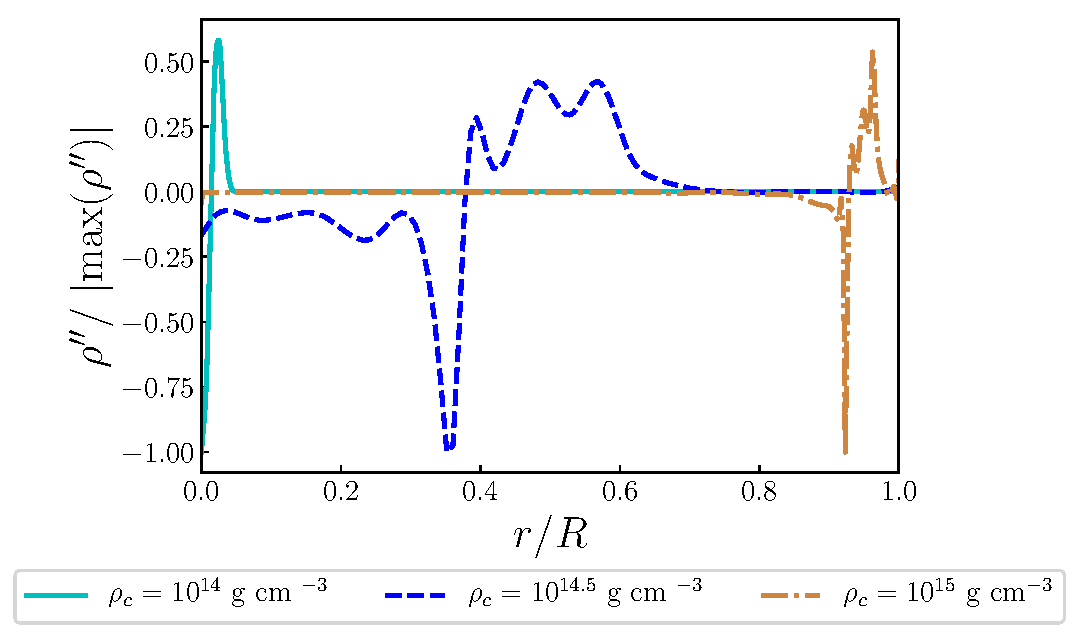
\includegraphics[width=0.8\linewidth]{figures/ConvecStabilityeng.pdf}
    \caption[Verificación de C11 para la EOS ENG]{Verificación de C11 para la EOS ENG. Se presenta $\rho^{\prime\prime}(r)$ de una muestra representativa de los modelos que cumplen con C10. La condición no se cumple en toda la estrella para todos los modelos. }
    \label{ConvecStabilityeng}
\end{figure}
\begin{figure}[H]
    \centering
    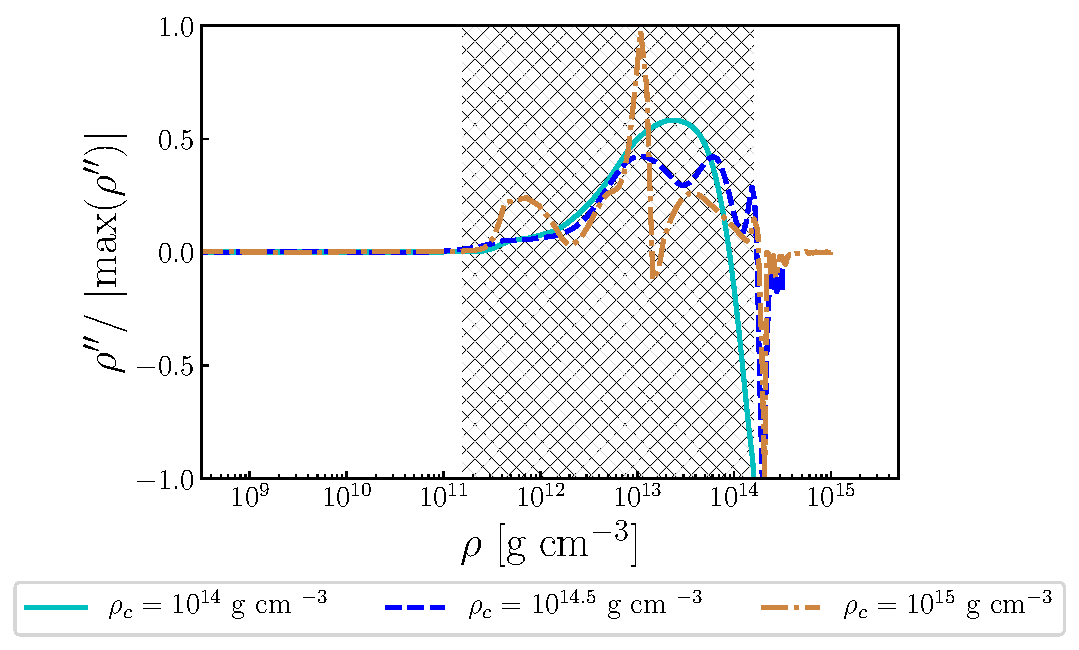
\includegraphics[width=0.8\linewidth]{figures/ConvecStabilityengCorrel.pdf}
    \caption[Correlación entre la inestabilidad y la corteza interior usando el diagrama $\rho^{\prime\prime}$ vs $\rho$]{El gráfico $\rho^{\prime\prime}(\rho)$ permite identificar la ubicación de las inestabilidades: para todos los modelos se encuentran en el rango de densidades ($\rho_{ND},\rho_0$) (área sombreada), lo que pudiera indicar que se trata de la corteza interior de la estrella.} 
    \label{ConvecStabilityengCorrel}
\end{figure}


\section{Consolidados}
\noindent Inicialmente se graficaron las relaciones $M$-$R$ ( ver Figura\ref{MRrel}), este diagrama obtenido al graficar el radio $R$ y la masa $M$ en el borde de la estrella $r=R$ \ref{MRrel}, es una de las maneras más comunes de verificar que los resultados obtenidos son consistentes con los trabajos existentes. En este caso al comparar con lo presentado en \cite{Ozel2016} para el mismo conjunto de EOSs se aprecia esta consistencia entre los diagramas.

\begin{figure}[H]
    \centering
    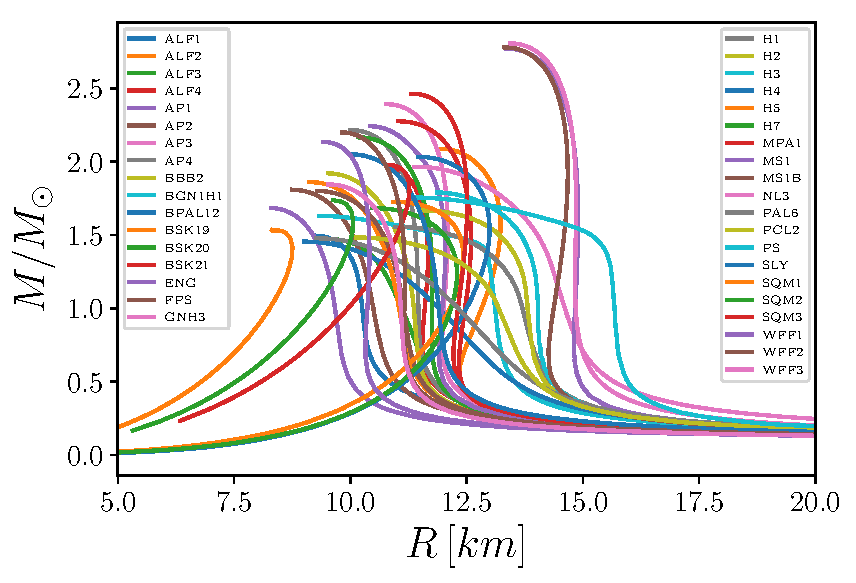
\includegraphics[width=0.8\linewidth]{figures/MRrels.pdf}
    \caption[Relaciones $M-R$]{Relaciones $M$-$R$ para todas las ecuaciones de estado consideradas. Esta gráfica puede ser contrastada con las relaciones $M-R$ presentadas en la Figura 7 de \cite{Ozel2016}.} 
    \label{MRrel}
\end{figure}

Seguido a esto se realizó un análisis análogo al presentado en la sección anterior para todo el conjunto de 37 EOSs. Los resultados fueron sintetizados en la Tabla \ref{Consolidados} y pueden ser consultados en el notebook de Jupyter RAnalysis \footnote{\url{https://nbviewer.jupyter.org/github/DavidRamosSal/stellar_structure/blob/master/RAnalysis.ipynb}}. 

\begin{table}[H]
\caption[Resultados consolidados]{\small Resultados para las 37 EOSs realistas consideradas. C6: condición de energía dominante, C7: causalidad, C11: movimientos convectivos. Se listan además el método teórico usado para obtener la EOS, los componentes que interactúan fuertemente (todos los modelos incluyen contribuciones leptónicas), la masa máxima $M_{\text{max}}$ con el respectivo radio $R_{M_{\text{max}}}$ para estrellas estáticas y la referencia a los trabajos originales.}
\label{Consolidados}
\begin{adjustbox}{max width=\textwidth}
\begin{tabular}{ccccccccccc}
\hline
\multirow{2}{*}{\textbf{EOS}} & \multirow{2}{*}{\textbf{Método}}           & \multirow{2}{*}{\textbf{Composición}} & \multirow{2}{*}{\begin{tabular}[c]{@{}c@{}}$\mathbf{M}_{\text{\textbf{max}}}$\\  $[\mathbf{M_{\odot}}]$\end{tabular}} & \multirow{2}{*}{\begin{tabular}[c]{@{}c@{}}$\mathbf{R}_{\mathbf{M}_{\text{\textbf{max}}}}$\\  $[$\textbf{km}$]$\end{tabular}} & \multirow{2}{*}{\textbf{C6}} & \multirow{2}{*}{\textbf{C7}}  & \multirow{2}{*}{\textbf{C11}} & \multirow{2}{*}{\textbf{Referencia}}          \\
                     &                                   &                              &                                                                                            &                                                                                                           &                     &                                         &                      &                                      \\ \hline \addlinespace
ALF1                 & \multirow{4}{*}{Mixto}            & \multirow{4}{*}{$n,p,q$}     & 1.496                                                                                      & 9.221                                                                                              & \checkmark          & \checkmark                    & \Cross               & \multirow{4}{*}{\cite{Alford2005}}   \\
ALF2                 &                                   &                              & 2.087                                                                                      & 11.962                                                                                              & \checkmark          & \checkmark                    & \Cross               &                                      \\
ALF3                 &                                   &                              & 1.473                                                                                      & 9.514                                                                                               & \checkmark          & \checkmark                    & \Cross               &                                      \\
ALF4                 &                                   &                              & 1.943                                                                                      & 10.892                                                                                              & \checkmark          & \checkmark                    & \Cross               &                                      \\ \addlinespace
AP1                  & \multirow{4}{*}{Variacional}      & \multirow{4}{*}{$n,p$}       & 1.684                                                                                      & 8.292                                                                                               & \checkmark          & \checkmark                    & \Cross               & \multirow{4}{*}{\cite{Akmal1998}}    \\
AP2                  &                                   &                              & 1.809                                                                                      & 8.746                                                                                               & \checkmark          & \Cross                        & \Cross               &                                      \\
AP3                  &                                   &                              & 2.391                                                                                      & 10.765                                                                                              & \Cross              & \Cross                        & \Cross               &                                      \\
AP4                  &                                   &                              & 2.214                                                                                      & 10.004                                                                                              & \Cross              & \Cross                        & \Cross               &                                      \\ \addlinespace
BBB2                 & BD-HF                     & $n,p$                        & 1.920                                                                                      & 9.515                                                                                               & \checkmark          & \checkmark                    & \Cross               & \cite{Lombardo2004}                  \\ \addlinespace
BGN1H1               & Potencial efectivo                & $n,p,H$                      & 1.630                                                                                      & 9.325                                                                                               & \checkmark          & \checkmark                    & \Cross               & \cite{Balberg1997}                   \\ \addlinespace
BPAL12               & BD-HF                     & $n,p$                        & 1.455                                                                                      & 9.015                                                                                               & \checkmark          & \checkmark                    & \Cross               & \cite{Zuo1999}                       \\ \addlinespace
BSK19                & \multirow{3}{*}{Potencial efectivo}              & \multirow{3}{*}{$n,p$}       & 1.861                                                                                      & 9.110                                                                                               & \Cross              & \Cross                        & \Cross               & \multirow{3}{*}{\cite{Potekhin2013}} \\
BSK20                &                                   &                              & 2.165                                                                                      & 10.173                                                                                              & \Cross              & \Cross                        & \Cross               &                                      \\
BSK21                &                                   &                              & 2.274                                                                                      & 11.038                                                                                              & \Cross              & \Cross                        & \Cross               &                                      \\ \addlinespace
ENG                  & BD-HF                     & $n,p$                        & 2.241                                                                                      & 10.425                                                                                              & \checkmark          & \checkmark                    & \Cross               & \cite{Engvik1994}                    \\ \addlinespace
FPS                  & Variacional                       & $n,p$                        & 1.800                                                                                      & 9.279                                                                                               & \checkmark          & \checkmark                    & \Cross               & \cite{Friedman1981}                  \\ \addlinespace
GNH3                 & Teoría de campos                  & $n,p,H,\Delta$               & 1.965                                                                                      & 11.372                                                                                              & \checkmark          & \checkmark                    & \Cross               & \cite{Glendenning1985}               \\ \addlinespace
H1                   & \multirow{6}{*}{Teoría de campos} & \multirow{6}{*}{$n,p,H$}     & 1.556                                                                                      & 10.968                                                                                              & \checkmark          & \checkmark                    & \Cross               & \multirow{6}{*}{\cite{Lackey2006}}   \\
H2                   &                                   &                              & 1.668                                                                                      & 11.516                                                                                              & \checkmark          & \checkmark                    & \Cross               &                                      \\
H3                   &                                   &                              & 1.790                                                                                      & 11.863                                                                                              & \checkmark          & \checkmark                    & \Cross               &                                      \\
H4                   &                                   &                              & 2.032                                                                                      & 11.467                                                                                              & \checkmark          & \checkmark                    & -           &                                      \\
H5                   &                                   &                              & 1.726                                                                                      & 10.930                                                                                              & \checkmark          & \checkmark                    &  -           &                                      \\
H7                   &                                   &                              & 1.683                                                                                      & 10.474                                                                                              & \checkmark          & \checkmark                    & -           &                                      \\ \addlinespace

 \hline \addlinespace
\multicolumn{1}{l}{} & \multicolumn{1}{l}{}              & \multicolumn{1}{l}{}         & \multicolumn{1}{l}{}                                                                       & \multicolumn{1}{l}{}                                                                      & \multicolumn{1}{l}{} & \multicolumn{1}{l}{} & \multicolumn{4}{l}{\small{(Continúa en la siguiente página)}} 
\end{tabular}
\end{adjustbox}
\end{table}


% Please add the following required packages to your document preamble:
% \usepackage{multirow}
\begin{table}[H]
\renewcommand\thetable{3.1 (continuación)}
\caption[]{}
\begin{adjustbox}{max width=\textwidth}
\begin{tabular}{ccccccccccc}
\hline
\multirow{2}{*}{\textbf{EOS}} & \multirow{2}{*}{\textbf{Método}}           & \multirow{2}{*}{\textbf{Composición}} & \multirow{2}{*}{\begin{tabular}[c]{@{}c@{}}$\mathbf{M}_{\text{\textbf{max}}}$\\  $[\mathbf{M_{\odot}}]$\end{tabular}} & \multirow{2}{*}{\begin{tabular}[c]{@{}c@{}}$\mathbf{R}_{\mathbf{M}_{\text{\textbf{max}}}}$\\  $[$\textbf{km}$]$\end{tabular}}  & \multirow{2}{*}{\textbf{C6}} & \multirow{2}{*}{\textbf{C7}}  & \multirow{2}{*}{\textbf{C11}} & \multirow{2}{*}{\textbf{Referencia}}          \\
                     &                                   &                              &                                                                                            &                                                                                                                &                     &                                          &                      &                                      \\ \hline \addlinespace
MPA1                 & BD-HF                     & $n,p$                        & 2.462                                                                                      & 11.301                                                                                              & \checkmark          & \checkmark                    & \Cross               & \cite{Muther1987}                    \\ \addlinespace
MS1                  & \multirow{2}{*}{Teoría de campos} & \multirow{2}{*}{$n,p$}       & 2.770                                                                                      & 13.346                                                                                              & \checkmark          & \checkmark                    & \Cross               & \multirow{2}{*}{\cite{Muller1996}}   \\
MS1b                 &                                   &                              & 2.778                                                                                      & 13.301                                                                                              & \checkmark          & \checkmark                    & \Cross               &                                      \\ \addlinespace
NL3                  & Teoría de campos                  & $n,p,\sigma,\omega,\rho$     & 2.806                                                                                      & 13.427                                                                                              & \checkmark          & \checkmark                    & \Cross               & \cite{Lalazissis1997}                \\ \addlinespace
PAL6                 & Potencial esquemático                             & $n,p$                        & 1.478                                                                                      & 9.258                                                                                               & \checkmark          & \checkmark                    & \Cross               & \cite{Prakash1988}                   \\ \addlinespace
PCL2                 & Teoría de campos                  & $n,p,H,q$                    & 1.483                                                                                      & 10.116                                                                                              & \checkmark          & \checkmark                    & \Cross               & \cite{Prakash1995}                   \\ \addlinespace
PS                   & Teoría de campos                  & $n,\pi^0$                    & 1.755                                                                                      & 11.372                                                                                              & \checkmark          & \checkmark                    & \Cross               & \cite{Pandharipande1975}             \\ \addlinespace
SLy                  & Mixto                             & $n,p$                        & 2.050                                                                                      & 9.977                                                                                               & \checkmark          & \Cross                        & \Cross               & \cite{Douchin2001}                   \\ \addlinespace
SQM1                 & \multirow{3}{*}{Teoría de campos} & \multirow{3}{*}{$q$}         & 1.532                                                                                      & 8.315                                                                                               & \checkmark          & \checkmark                    & -*                    & \multirow{3}{*}{\cite{Prakash1995}}  \\
SQM2                 &                                   &                              & 1.737                                                                                      & 9.638                                                                                               & \checkmark          & \checkmark                    & -*                    &                                      \\
SQM3                 &                                   &                              & 1.977                                                                                      & 10.814                                                                                              & \checkmark          & \checkmark                    & -*                    &                                      \\ \addlinespace
WFF1                 & \multirow{3}{*}{Variacional}      & \multirow{3}{*}{$n,p$}       & 2.134                                                                                      & 9.413                                                                                               & \checkmark          & \Cross                        & \Cross               & \multirow{3}{*}{\cite{Wiringa1988}}  \\
WFF2                 &                                   &                              & 2.199                                                                                      & 9.825                                                                                               & \checkmark          & \Cross                        & \Cross               &                                      \\
WFF3                 &                                   &                              & 1.845                                                                                      & 9.516                                                                                               & \checkmark          & \checkmark                    & \Cross               &                                      \\ \addlinespace \hline \addlinespace
\multicolumn{3}{l}{\small{*Resultados con problemas en la frontera}}                                            & \multicolumn{1}{l}{}                                                                       & \multicolumn{1}{l}{}                                                                      & \multicolumn{1}{l}{} & \multicolumn{1}{l}{} & \multicolumn{1}{l}{} & \multicolumn{1}{l}{} & \multicolumn{1}{l}{} & \multicolumn{1}{l}{}             
\end{tabular}
\end{adjustbox}
\end{table}

 En primer lugar se encontró que todas las EOSs consideradas producen modelos estelares que son estables ante cracking. Se encontró que 31 de las 37 EOSs producen modelos estelares que presentan inestabilidades convectivas en la corteza interior (comportamiento descrito en la Figura \ref{ConvecStabilityengCorrel} en el mismo rango de densidades).

Seis EOSs (H4-7,SQM1-3) no pudieron ser evaluadas rigurosamente pues las tablas sólo contenían la parte más densa de la EOS ($\rho > 10^{14}$ g cm$^{-3}$), presuntamente para ser acoplada posteriormente con una EOS para la corteza. 

Además, los valores de $M_{\text{max}}$ y el respectivo radio $R_{M_{\text{max}}}$ calculados para cada EOS son cercanos a los obtenidos en \cite{Read2009} para un conjunto similar de EOSs y representan por lo tanto otra forma de validar los cálculos. Sin embargo, como este trabajo está orientado al análisis de los perfiles de densidad y presión, no se procederá a calcular diferencias para estos parámetros entre las dos simulaciones.

\section{Discusión}

\noindent A continuación se presentará una discusión sobre los resultados encontrados para las condiciones de aceptabilidad evaluada.



\emph{C6: condición de energía dominante} y \emph{C7: Causalidad}. Tras encontrar que EOSs usadas ampliamente en aplicaciones no cumplen estas condiciones surge la pregunta: ¿puede una EOS físicamente correcta violar C6 y C7? De acuerdo a \cite{Haensel2007} existen ejemplos de modelos que a pesar de no cumplir C6 y C7 siguen siendo causales e invariantes ante transformaciones de Lorentz. Sin embargo, el hecho de que los modelos que no cumplen estas condiciones están basados en esquemas de muchos cuerpos no relativistas sugiere que los modelos son artificiales pues este tipo de comportamientos no se presenta en esquemas relativistas. Además, se encontró que todas las ecuaciones que no cumplen C6 tampoco cumplen C7, mientras que lo opuesto no se cumple, esto sugiere que otras características aparte de la rigidez de la EOS pueden resultar en violaciones a C7. Por otro lado se ha sugerido que la condición C7 se debe cumplir sólo a densidades realizables en las estrellas de neutrones \cite{Douchin2001}, esto es, a densidades menores a la densidad para la que se obtiene la masa máxima. Si esto es correcto, algunas de las EOS que cumplen C6 pero no C7 seguirían siendo físicamente aceptables, pero no se intentará resolver ese problema en este trabajo.


\emph{C11: convección adiabática}. Los resultados indican que según el criterio C11 la corteza interior de las estrellas de neutrones es inestable ante convección, para todas las EOSs consideradas. Previamente en \cite{Miralles1997} se mostró que en estrellas débilmente magnetizadas, la envoltura de la estrella de neutrones puede ser inestable ante convección. Sin embargo, nada se ha reportado acerca de la estabilidad de la corteza interior. Es sabido \cite{Haensel2007} que las transiciones de fase primer orden que ocurren en la interfaz corteza-núcleo producen discontinuidades en el perfil de densidad, esto es observado en los resultados (pico en regiones con densidades cercanas a $\rho_0$ en la Figura \ref{ConvecStabilityengCorrel}) y puede tener algo que ver con la existencia de la inestabilidad en regiones que se acercan a estas densidades.

\vspace{0.3cm}
\noindent\textbf{Sobre el criterio de estabilidad C8}

\begin{figure}%[H]
    \centering
    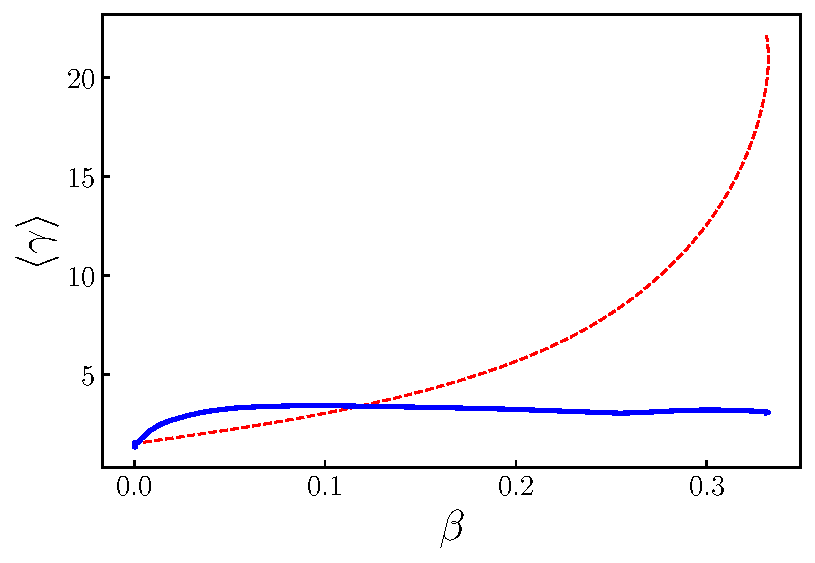
\includegraphics[width=0.6\linewidth]{figures/AdiabaticIndexENGbeta.pdf}
    \caption[Estabilidad usando el índice adiabático]{Verificación de C8 para la EOS ENG. La línea roja punteada representa $\gamma_{cr}$. La igualdad $\langle \gamma \rangle$ no se alcanza para la compacidad de la configuración de masa máxima ($\beta_{cr}=0.317$ en este caso) como es presentado en \cite{Koliogiannis2019a}, debido al rápido crecimiento de $\gamma_{cr}$.} 
    \label{AdiabaticIndexCriterio}
\end{figure}

\noindent Recientemente \cite{Koliogiannis2019a} se usó la restricción que impone este criterio sobre el índice adiabático efectivo $\langle \gamma \rangle$ para obtener una relación entre la compacidad de la configuración con masa máxima $\beta_{cr}$ y el índice adiabático $\gamma_{cr}$, que es independiente de la EOS. Sin embargo, los resultados encontrados arrojan un crecimiento muy rápido $\gamma_cr$ con la compacidad $\beta$ para todas las EOSs (ver la Figura \ref{AdiabaticIndexCriterio} para un ejemplo) que no predice la igualdad $\langle \gamma \rangle = \gamma_{cr}$ para el valor de $\beta_{cr}$.

Este resultado es preliminar y se espera verificar que las integrales presentes en el cálculo de $\gamma_{cr}$ \eqref{gammacrit} no estén introduciendo un error numérico.
\chapter{Conclusiones}
%El comportamiento de la materia en las estrellas de neutrones 
%Al día de hoy nuestra comprensión de las leyes de la física a densidades altas sigue siendo pobre. 
%La EOS de la materia en el interior de las estrellas de neutrones sigue siendo al día de hoy un misterio. Además de su importancia práctica en simulaciones de diferentes eventos astrofísicos,
\noindent Más allá de su utilidad práctica en simulaciones de supernovas y otros eventos astronómicos, la importancia de determinar la EOS de la materia al interior de las estrellas de neutrones reside en que nos permite entender el comportamiento de las leyes de la física a densidades que no son realizables experimentalmente en la tierra. La existencia de múltiples candidatos sólo refleja nuestra inhabilidad para aplicar nuestro conocimiento de física nuclear en condiciones tan extremas como las encontradas en las estrellas de neutrones. El objetivo de este trabajo fue aplicar criterios de aceptabilidad física a los modelos de estrellas de neutrones estáticas obtenidos con diferentes EOSs con el fin de identificar candidatos que produzcan modelos que no sean realistas. 

Tras una breve discusión sobre los aspectos generales de las estrellas de neutrones, se presentó una deducción de las ecuaciones de estructura estelar tanto en la teoría Newtoniana como en la relativista y se explicó cómo brindando una EOS es posible construir modelos estelares. Las condiciones de aceptabilidad fueron presentadas y aplicadas a un conjunto de 37 EOSs que varían ampliamente en composición y rigidez. En lo que concierne a las condiciones C1-10 los resultados obtenidos en este trabajo habían sido presentados en los artículos originales y parcialmente en otros trabajos \cite{Ozel2016,Read2009}, excepto para la condición C4: el problema encontrado al aplicar los criterios existentes para restringir el valor del índice adiabático al interior de la estrella no ha sido reportado. 

Los resultados obtenidos para la condición C11 fueron inesperados: la corteza interior de los modelos obtenidos con todas las EOSs consideradas es inestable ante movimientos convectivos adiabáticos. La posibilidad de que la corteza interna presente inestabilidades convectivas no ha sido reportada antes y debido a la complejidad de los modelos físicos desarrollados para describir fenómenos como la superfluidez y cambios de fase que ocurren esta región, es difícil identificar posibles causas. Este resultado puede ser importante dado que se cree que existe convección de superfluido de esta región hacia otras \cite{Haensel2007}. 

Respecto a la confiabilidad de los resultados obtenidos cabe resaltar que la rutina numérica reproduce diferentes soluciones exactas de fluido perfecto con gran precisión y que los problemas de usar diferencias finitas para calcular derivadas numéricas fueron superados con la ayuda de un spline con un factor de suavizamiento. Así mismo, los resultados de la masas máximas y los respectivos radios para cada EOS concuerdan con lo presentado en otros trabajos.

Una de las inquietudes que puede surgir al aplicar el criterio C11 a modelos de estrellas de neutrones es que éste es Newtoniano en esencia (es una consecuencia directa del principio de Arquímedes) y su validez en el contexto de la relatividad general no está asegurada. Sin embargo, como ha sido argumentado para criterios de estabilidad ante convección Newtonianos más generales, a diferencia de las pulsaciones que son fenómenos globales, la inestabilidad ante convección es un fenómeno local que está gobernado enteramente por los valores locales de las variables termodinámicas \cite{Thorne1966}.    

La metodología de este trabajo es análoga a la presentada en \cite{Delgaty1998} para soluciones exactas y, en vista del resultado obtenido para la estabilidad convectiva, complementa el uso de observaciones para restringir modelos de EOSs de una manera fundamental, puesto que permite identificar partes específicas del conocimiento actual en las que es posible no se haya explorado todo el rango de posibilidades físicas.

Finalmente, se espera extender el trabajo realizado para incluir más EOSs, incluyendo modernas EOSs de "alta precisión" que permitirían reducir los errores numéricos inherentes a la interpolación y analizar mejor la estabilidad de la corteza interior.


\clearpage
% This displays the bibliography for all cited external documents. All references have to be defined in the file references.bib and can then be cited from within this document.
%kai
\bibliographystyle{apacite}

\bibliography{references}
%\TODO{Chequear que los links estén correctos.}
\addcontentsline{toc}{chapter}{Referencias Bibliogr\'aficas}

% This creates an appendix chapter, comment if not needed.

\appendix
\addcontentsline{toc}{chapter}{Apéndice}

\chapter{Curvatura de un espacio-tiempo estático con simetría esférica}\label{curvature}

\anexo{Curvatura de un espacio-tiempo est\'atico con simetr\'ia esf\'erica}\label{anexoA}
\addcontentsline{loa}{chapter}{Introducción}

\noindent \small \textbf{Nota:} Las \quotes{$\dd$}s representarán derivadas exteriores y se usarán cantidades primadas para denotar derivación respecto a $r$.

\normalsize
\noindent La métrica de un espacio-tiempo estático con simetría esférica está dada por
\begin{equation}
    \bm{g}=-e^{2 a(r)} \dd{t} \otimes \dd{t}+e^{2 b(r)} \dd{r} \otimes \dd{r} +r^{2}\left(\dd{\theta} \otimes \dd{\theta}+\operatorname{sen}^{2} \theta \dd{\varphi} \otimes \dd{\varphi}\right).
\end{equation}
El tensor de curvatura de Riemann correspondiente a esta métrica puede ser calculado de manera simple haciendo uso del cálculo de Cartan (cf. \cite{Chandrasekhar1983,Straumann2013}). 

En el cálculo de Cartan se hace uso del hecho de que es posible escoger como base del espacio cotangente $T^{*}_p$ en un punto $p$ de la variedad, una base $\omega^{\alpha}$ diferente a la base coordenada $\dd{x^\alpha}$. Esta base se escoge de modo tal que la métrica pueda ser escrita como 
\begin{equation}
    \bm{g}=\tensor{\eta}{_\alpha_\beta} \omega^{\alpha} \otimes \omega^{\beta},
\end{equation}
donde $\tensor{\eta}{_\alpha_\beta}$ es la métrica de Minkowski. Este tipo de bases se conocen como bases ortonormales. 
Con lo anterior en mente, se define la tétrada de 1-formas base como
%\begin{subequations}
\begin{equation}
    \omega^0=\,e^{a}\dd{t}, \quad
    \omega^1=\,e^{b}\dd{r}, \quad
    \omega^2=\,r\dd{\theta}, \quad
    \omega^3=\,r\sen{\theta}\dd{\varphi}.
    \label{tetrada}
\end{equation}
%\end{subequations}
Usando las ecuaciones de estructura de Cartan para un espacio-tiempo sin torsión
\begin{subequations}
\begin{align}
    \dd{\omega^\alpha} =& -\tensor{\Gamma}{^\alpha_ \mu} \wedge \omega^{\mu}\,, \label{1SE}\\
    \tensor{\Omega}{^\alpha_\beta} =& \dd{ \tensor{\Gamma}{^\alpha_\beta}} + \tensor{\Gamma}{^\alpha_\mu}  \wedge \tensor{\Gamma}{^\mu_\beta}\,, \label{2SE}
\end{align}
\end{subequations}
donde $\tensor{\Gamma}{^\alpha_\beta}$ son las 1-formas de conexión, las cuales cumplen 
\begin{equation}
    \Gamma_{\alpha \beta}+\Gamma_{\alpha \beta}=0. \label{skew}
\end{equation}
A partir de las ecuaciones de estructura \eqref{1SE} y \eqref{2SE} se pueden obtener las 2-formas de curvatura $\tensor{\Omega}{^\alpha_\beta}$ y a partir de estas, las componentes del tensor de Riemann ya que por definición 
\begin{equation}
    \tensor{\Omega}{^\alpha_\beta}=\frac{1}{2}\tensor{R}{^\alpha_\beta_\mu_\nu}\omega^\mu \wedge \omega^\nu.
\end{equation}
Comenzando por el cálculo de las 1-formas de conexión, se hallan las derivadas exteriores de la tétrada \eqref{tetrada}
    \begin{align}
    \begin{split}
        \dd{\omega^0}=&\dd{e^a} \wedge \dd{t}+e^a\cancelto{0}{\dd{(\dd{t})}} = a^{\prime} e^a \dd{r}\wedge\dd{t} = -a^{\prime} e^{-b} \omega^0 \wedge \omega^1, \\
        \dd{\omega^1}=&\dd{e^b}\wedge\dd{r}+e^b\cancelto{0}{\dd{(\dd{r})}} = b^{\prime}e^b\dd{r}\wedge\dd{r}=0, \\
        \dd{\omega^2}=&\dd{r}\wedge\dd{\theta} + r\cancelto{0}{\dd{(\dd{\theta})}} = -\frac{e^{-b}}{r}\omega^2 \wedge\omega^1, \\
        \dd{\omega^3}=&\dd{(rsen\theta)}\wedge\dd{\varphi} + r\sen{\theta}\cancelto{0}{\dd{(\dd{\varphi})}} = \sen{\theta}\dd{r}\wedge\dd{\varphi} + r\cos{\theta}\dd{\theta}\wedge\dd{\varphi} \\
        & \phantom{{}\dd{(rsen\theta)}\wedge\dd{\varphi} + r\sen{\theta}\cancelto{0}{\dd{(\dd{\varphi})}}} = -\frac{e^{-b}}{r} \omega^3 \wedge \omega^1 - \frac{\cot{\theta}}{r} \omega^3 \wedge \omega^2.
    \end{split}
    \end{align}
reemplazando en la primera ecuación de estructura \eqref{1SE} se obtiene
    \begin{equation*}
        \tensor{\Gamma}{^0_0}\wedge\omega^0 + \tensor{\Gamma}{^0_1}\wedge\omega^1+\tensor{\Gamma}{^0_2}\wedge\omega^2+\tensor{\Gamma}{^0_3}\wedge\omega^3 = \,a^{\prime} e^{-b} \omega^0 \wedge \omega^1 \hspace*{3.6cm}
    \end{equation*}
    \begin{align}
    \begin{split}
        \tensor{\Gamma}{^1_0}\wedge\omega^0 + \tensor{\Gamma}{^1_1}\wedge\omega^1+\tensor{\Gamma}{^1_2}\wedge\omega^2+\tensor{\Gamma}{^1_3}\wedge\omega^3 =&\, 0, \\
        \tensor{\Gamma}{^2_0}\wedge\omega^0 + \tensor{\Gamma}{^2_1}\wedge\omega^1+\tensor{\Gamma}{^2_2}\wedge\omega^2+\tensor{\Gamma}{^2_3}\wedge\omega^3 =& \frac{e^{-b}}{r}\omega^2 \wedge\omega^1, \\
        \tensor{\Gamma}{^0_0}\wedge\omega^0 + \tensor{\Gamma}{^3_1}\wedge\omega^1+\tensor{\Gamma}{^3_2}\wedge\omega^2+\tensor{\Gamma}{^3_3}\wedge\omega^3 =& \frac{e^{-b}}{r} \omega^3 \wedge \omega^1 + \frac{\cot{\theta}}{r} \omega^3 \wedge \omega^2.
        \end{split}\label{1ee}
    \end{align}    
Teniendo en cuenta que la condición \eqref{skew} implica las relaciones 
\begin{equation*}
    \tensor{\Gamma}{^0_0}=0,\quad \tensor{\Gamma}{^0_i} = \tensor{\Gamma}{^i_0}, \quad \tensor{\Gamma}{^i_i} = 0, \quad \tensor{\Gamma}{^i_j} = -\tensor{\Gamma}{^j_i},
\end{equation*}
de \eqref{1ee} se obtienen que las 1-formas de conexión no nulas son
\begin{subequations}
    \begin{align}
        \tensor{\Gamma}{^0_1} =& \,\tensor{\Gamma}{^1_0} = a^{\prime} e^{-b} \omega^0, \label{1fa} \\
        \tensor{\Gamma}{^2_1} =& -\tensor{\Gamma}{^1_2} = \frac{e^{-b}}{r}\omega^2, \label{1fb} \\
        \tensor{\Gamma}{^3_1} =& -\tensor{\Gamma}{^1_3} = \frac{e^{-b}}{r}\omega^3, \label{1fc} \\
        \tensor{\Gamma}{^3_2} =& -\tensor{\Gamma}{^2_3} = \frac{\cot{\theta}}{r} \omega^3. \label{1fd}
    \end{align}
\end{subequations}


Hallando las derivadas exteriores de \eqref{1fa}--\eqref{1fd} 
\begingroup
\allowdisplaybreaks
\begin{subequations}
    \begin{align}
        \dd{\tensor{\Gamma}{^0_1}} =& \dd{(a^\prime e^{-b})}\wedge\omega^0 + a^\prime e^{-b}\dd{\omega^0} \nonumber \\
        =& e^{-b}\dd{(a^\prime)}\wedge\omega^0 + a^\prime \dd{(e^{-b})}\wedge\omega^0-a^{\prime 2} e^{-2b}\omega^0\wedge\omega^1 \nonumber \\
        =& a^{\prime\prime} e^{-b} \dd{r}\wedge\omega^0 -a^{\prime}b^{\prime}e^{-b}\dd{r}\wedge\omega^0-a^{\prime 2}e^{-2b}\omega^0\wedge\omega^1 \nonumber \\
        =& e^{-2b}(a^{\prime\prime}+a^{\prime 2}-a^\prime b^\prime) \omega^1 \wedge \omega^0, \\
        \dd{\tensor{\Gamma}{^2_1}} =& \dd{\left(\frac{e^{-b}}{r}\right)}\wedge\omega^2 + \frac{e^{-b}}{r}\dd{\omega^2} \nonumber \\
        =& \frac{1}{r}\dd{e^{-b}}\wedge\omega^2 + e^{-b} \dd{\left(\frac{1}{r}\right)}\wedge\omega^2 + \frac{e^{-2b}}{r^2}\omega^1 \wedge \omega^2 \nonumber \\
        =& -\frac{b^\prime}{r}e^{-b}\dd{r}\wedge\omega^2 -\cancel{\frac{e^{-b}}{r^2}\dd{r}\wedge\omega^2} +\cancel{\frac{e^{-2b}}{r^2}\omega^1\wedge\omega^2} \nonumber \\
        =& - \frac{b^\prime e^{-2b}}{r} \omega^1 \wedge \omega^2, \\
        \dd{\tensor{\Gamma}{^2_1}} =& \dd{\left(\frac{e^{-b}}{r}\right)}\wedge\omega^3 + \frac{e^{-b}}{r}\dd{\omega^3} \nonumber \\
        =& \frac{1}{r}\dd{\left(e^{-b}\right)}\wedge\omega^3 + e^{-b}\dd{\left(\frac{1}{r}\right)}\wedge\omega^3+\frac{e^{-2b}}{r^2}\omega^1\wedge\omega^3 + \frac{e^-b}{r^2}\cot{\theta}\omega^2\wedge\omega^3 \nonumber \\
        =& -\frac{b^\prime e^{-2b}}{r}\dd{r}\wedge\omega^3-\cancel{\frac{e^{-b}}{r^2}\dd{r}\wedge\omega^3} + \cancel{\frac{e^{-2b}}{r^2}\omega^1\wedge\omega^3}+\frac{e^{-b}}{r^2}\cot{\theta}\omega^2\wedge\omega^3 \nonumber \\
        =& -\frac{b^\prime e^{-2b}}{r}\omega^1\wedge\omega^3 + \frac{e^{-b}\cot{\theta}}{r^2}\omega^2\wedge\omega^3, \\
        \dd{\tensor{\Gamma}{^3_2}}=& \dd{\left( \frac{\cot{\theta}}{r} \right)}\wedge\omega^3 + \frac{\cot{\theta}}{r}\dd{\omega^3} \nonumber \\ 
        =& \frac{1}{r}\dd{\qty(\cot{\theta})}+\cot{\theta}\dd{\qty(\frac{1}{r})}\wedge\omega^3 \nonumber \\
        =& -\frac{\csc^2{\theta}}{r}\dd{\theta}\wedge\omega^3 -\cancel{ \frac{\cot{\theta}}{r^2}\dd{r}\wedge\omega^3}+\cancel{\frac{\cot{\theta}e^{-b}}{r^2}\omega^1\wedge\omega^3}+\frac{\cot^2{\theta}}{r^2}\omega^2\wedge\omega^3 \nonumber \\
        =& \frac{1}{r^2}\cancelto{-1}{(\cot^2{\theta}-\csc^2{\theta})}\omega^2\wedge\omega^3 \nonumber \\
        =& -\frac{1}{r^2}\omega^2\wedge\omega^3.
    \end{align}
\end{subequations}
\endgroup
Reemplazando las 1-formas de conexión y sus derivadas exteriores en la segunda ecuación de estructura \eqref{2SE} se obtienen las 2-formas de curvatura $\tensor{\Omega}{^\alpha_\beta}$
\begingroup
\allowdisplaybreaks
\begin{subequations}
    \begin{align}
        \tensor{\Omega}{^0_1}=&\dd{\tensor{\Gamma}{^0_1}}+\cancelto{0}{\tensor{\Gamma}{^0_0}}\wedge\tensor{\Gamma}{^0_1}+\tensor{\Gamma}{^0_1}\wedge\cancelto{0}{\tensor{\Gamma}{^1_1}}+\cancelto{0}{\tensor{\Gamma}{^0_2}}\wedge\tensor{\Gamma}{^2_1}+\cancelto{0}{\tensor{\Gamma}{^0_3}}\wedge\tensor{\Gamma}{^3_1} \nonumber \\
        =& -e^{-2b}(a^{\prime\prime}+a^{\prime 2}-a^\prime b^\prime)\omega^0\wedge\omega^1 = \frac{1}{2}\tensor{R}{^0_1_\alpha_\beta}\omega^\alpha\wedge\omega^\beta, \\
        \tensor{\Omega}{^0_2}=&\dd{\cancelto{0}{\tensor{\Gamma}{^0_2}}}+\cancelto{0}{\tensor{\Gamma}{^0_0}}\wedge\tensor{\Gamma}{^0_2}+\tensor{\Gamma}{^0_1}\wedge\tensor{\Gamma}{^1_2}+\cancelto{0}{\tensor{\Gamma}{^0_2}}\wedge\cancelto{0}{\tensor{\Gamma}{^2_2}}+\cancelto{0}{\tensor{\Gamma}{^0_3}}\wedge\tensor{\Gamma}{^3_2} \nonumber \\
        =& -\frac{a^\prime e^{-2b}}{r}\omega^0\wedge\omega^2= \frac{1}{2}\tensor{R}{^0_2_\alpha_\beta}\omega^\alpha\wedge\omega^\beta, \\
        \tensor{\Omega}{^0_3}=&\dd{\cancelto{0}{\tensor{\Gamma}{^0_3}}}+\cancelto{0}{\tensor{\Gamma}{^0_0}}\wedge\cancelto{0}{\tensor{\Gamma}{^0_3}}+\tensor{\Gamma}{^0_1}\wedge\tensor{\Gamma}{^1_3}+\cancelto{0}{\tensor{\Gamma}{^0_2}}\wedge\tensor{\Gamma}{^2_3}+\cancelto{0}{\tensor{\Gamma}{^0_3}}\wedge\cancelto{0}{\tensor{\Gamma}{^3_3}} \nonumber \\
        =& -\frac{a^\prime e^{-2b}}{r}\omega^0\wedge\omega^3= \frac{1}{2}\tensor{R}{^0_3_\alpha_\beta}\omega^\alpha\wedge\omega^\beta, \\
        \tensor{\Omega}{^1_2}=&\dd{\tensor{\Gamma}{^1_2}}+\tensor{\Gamma}{^1_0}\wedge\cancelto{0}{\tensor{\Gamma}{^0_2}}+\cancelto{0}{\tensor{\Gamma}{^1_1}}\wedge\tensor{\Gamma}{^1_2}+\tensor{\Gamma}{^1_2}\wedge\cancelto{0}{\tensor{\Gamma}{^2_2}}+\tensor{\Gamma}{^1_3}\wedge\tensor{\Gamma}{^3_2} \nonumber \\
        =& \frac{e^{-2b}}{r}\omega^1\wedge\omega^2-\frac{e^{-b}\cot{\theta}}{r^2}\cancelto{0}{\omega^3\wedge\omega^3} \nonumber \\
        =& \frac{b^\prime e^{-2b}}{r}\omega^1\wedge\omega^2 = \frac{1}{2}\tensor{R}{^1_2_\alpha_\beta}\omega^\alpha\wedge\omega^\beta, \\
        \tensor{\Omega}{^1_3}=&\dd{\tensor{\Gamma}{^1_3}}+\tensor{\Gamma}{^1_0}\wedge\cancelto{0}{\tensor{\Gamma}{^0_3}}+\cancelto{0}{\tensor{\Gamma}{^1_1}}\wedge\tensor{\Gamma}{^1_3}+\tensor{\Gamma}{^1_2}\wedge\tensor{\Gamma}{^2_3}+\tensor{\Gamma}{^1_3}\wedge\cancelto{0}{\tensor{\Gamma}{^3_3}} \nonumber \\
        =& \frac{b^\prime e^{-2b}}{r}\omega^1\wedge\omega^3-\cancel{\frac{e^{-b}\cot{\theta}}{r^2}\omega^2\wedge\omega^3}+\cancel{\frac{e^{-b}\cot{\theta}}{r^2}\omega^2\wedge\omega^3} \nonumber \\
        =& \frac{b^\prime e^{-2b}}{r}\omega^1\wedge\omega^3 = \frac{1}{2}\tensor{R}{^1_3_\alpha_\beta}\omega^\alpha\wedge\omega^\beta, \\
        \tensor{\Omega}{^2_3}=&\dd{\tensor{\Gamma}{^2_3}}+\cancelto{0}{\tensor{\Gamma}{^2_0}}\wedge\cancelto{0}{\tensor{\Gamma}{^0_3}}+\tensor{\Gamma}{^2_1}\wedge\tensor{\Gamma}{^1_3}+\cancelto{0}{\tensor{\Gamma}{^2_2}}\wedge\tensor{\Gamma}{^2_3}+\tensor{\Gamma}{^2_3}\wedge\cancelto{0}{\tensor{\Gamma}{^3_3}} \nonumber \\
        =& \frac{1}{r^2}\omega^2\wedge\omega^3-\frac{e^{-2b}}{r^2}\omega^2\wedge\omega^3 \nonumber \\
        =& \frac{1-e^{-2b}}{r^2}\omega^2\wedge\omega^3 = \frac{1}{2}\tensor{R}{^2_3_\alpha_\beta}\omega^\alpha\wedge\omega^\beta,
    \end{align}
\end{subequations}
\endgroup
y por inspección se obtienen las componentes independientes del tensor de Riemann

\begin{align*}
        \tensor{R}{^0_1_0_1} &= -e^{-2b}(a^{\prime\prime}+a^{\prime 2}-a^\prime b^\prime), \\
        \tensor{R}{^0_2_0_2} &= -\frac{a^\prime e^{-2b}}{r}, \\ 
        \tensor{R}{^0_3_0_3} &= -\frac{a^\prime e^{-2b}}{r}, \\
        \tensor{R}{^1_2_1_2} &= \frac{b^\prime e^{-2b}}{r}, \\
        \tensor{R}{^1_3_1_3} &= \frac{b^\prime e^{-2b}}{r}, \\
        \tensor{R}{^2_3_2_3} &= \frac{1-e^{-2b}}{r^2}.
\end{align*}
Usando la antisimetría en el primer y segundo par de índices
\begin{equation}
    \tensor{\eta}{_\mu_\alpha}\tensor{R}{^\mu_\beta_\gamma_\delta}=-\tensor{\eta}{_\mu_\beta}\tensor{R}{^\mu_\alpha_\gamma_\delta}\quad \text{y} \quad \tensor{R}{^\alpha_\beta_\gamma_\delta}=\tensor{R}{^\alpha_\beta_\delta_\gamma},
\end{equation}
se obtienen las componentes restantes
\begin{equation}
    \begin{split}
    \tensor{R}{^0_1_0_1} &= \tensor{R}{^1_0_0_1} = -\tensor{R}{^0_1_1_0} = -\tensor{R}{^1_0_1_0}, \\
    \tensor{R}{^0_2_0_2} &=  \tensor{R}{^2_0_0_2} = - \tensor{R}{^0_2_2_0} = - \tensor{R}{^2_0_2_0}, \\
    \tensor{R}{^0_3_0_3} &= \tensor{R}{^3_0_0_3} = -\tensor{R}{^0_3_3_0}=-\tensor{R}{^3_0_3_0},
    \end{split}
    \qquad
    \begin{split}
    \tensor{R}{^1_2_1_2} &= \tensor{R}{^2_1_2_1} = -\tensor{R}{^1_2_2_1}=-\tensor{R}{^2_1_1_2}, \\
    \tensor{R}{^1_3_1_3} &= \tensor{R}{^3_1_3_1} = -\tensor{R}{^1_3_3_1} = -\tensor{R}{^3_1_1_3}, \\
    \tensor{R}{^2_3_2_3} &= \tensor{R}{^3_2_3_2} = -\tensor{R}{^2_3_3_2} = -\tensor{R}{^3_2_2_3}.
    \end{split}
\end{equation}
Contrayendo el tensor de Riemann se halla el tensor de Ricci
\begin{equation}
    \tensor{R}{_\alpha_\beta}=\tensor{R}{^\mu_\alpha_\mu_\beta},
\end{equation}
cuyas componentes serán
\begin{subequations}
\begin{align}
    \tensor{R}{_0_0}&=\tensor{R}{^0_0_0_0} + \tensor{R}{^1_0_1_0} + \tensor{R}{^2_0_2_0} + \tensor{R}{^3_0_3_0} \nonumber \\
    &= \frac{2a^\prime-r a^\prime b^\prime +r a^{\prime 2}+r a^{\prime\prime}}{r}e^{-2b} \\
    \tensor{R}{_1_1}&=\tensor{R}{^0_1_0_1} + \tensor{R}{^1_1_1_1} + \tensor{R}{^2_1_2_1} + \tensor{R}{^3_1_3_1} \nonumber \\
    &=\frac{2b^\prime+r a^\prime b^\prime -r a^{\prime 2}-r a^{\prime\prime}}{r}e^{-2b} \\
    \tensor{R}{_2_2}&=\tensor{R}{^0_2_0_2} + \tensor{R}{^1_2_1_2} + \tensor{R}{^2_2_2_2} + \tensor{R}{^3_2_3_2} \nonumber \\
    &= -\frac{a^\prime e^{-2b}}{r}+\frac{b^\prime e^{-2b}}{r}+\frac{1-e^{-2b}}{r} \\
    \tensor{R}{_3_3}&=\tensor{R}{^0_3_0_3} + \tensor{R}{^1_3_1_3} + \tensor{R}{^2_3_2_3} + \tensor{R}{^3_3_3_3} \nonumber \\
    &= -\frac{a^\prime e^{-2b}}{r}+\frac{b^\prime e^{-2b}}{r}+\frac{1-e^{-2b}}{r}.
\end{align}
\end{subequations}
y el escalar de curvatura contrayendo el tensor de Ricci
\begin{align}
    R&=\tensor{\eta}{^\alpha^\beta} \tensor{R}{_\alpha_\beta} \nonumber \\
    &= \tensor{\eta}{^0^0} \tensor{R}{_0_0} + \tensor{\eta}{^1^1} \tensor{R}{_1_1} + \tensor{\eta}{^2^2} \tensor{R}{_2_2} + \tensor{\eta}{^3^3} \tensor{R}{_3_3} \nonumber \\
    &= 2\qty(\frac{b^\prime-a^\prime+r a^\prime b^\prime -r a^{\prime 2}-r a^{\prime\prime}}{r}e^{-2b}+\frac{b^\prime-a^\prime}{r}e^{-2b}+\frac{1-e^{-2b}}{r^2}).
\end{align}
El tensor de Einstein, definido como
\begin{equation}
    \bm{G}=\bm{R}-\frac{1}{2}R\bm{g},
\end{equation}
o en componentes mixtas
\begin{equation}
    \tensor{G}{^\alpha_\beta}=\tensor{R}{^\alpha_\beta}-\frac{1}{2}R\tensor{\delta}{^\alpha_\beta}=\tensor{\eta}{^\alpha^\mu}\tensor{R}{_\mu_\beta}-\frac{1}{2}R\tensor{\delta}{^\alpha_\beta},
\end{equation}
puede ser calculado usando los resultados anteriores
\begingroup
\allowdisplaybreaks
\begin{subequations}
\begin{align}
    \tensor{G}{^0_0} &=  \tensor{\eta}{^0^0}\tensor{R}{_0_0}-\frac{1}{2}R\tensor{\delta}{^0_0} \nonumber \\
    &= - \frac{2a^\prime-r a^\prime b^\prime +r a^{\prime 2}+r a^{\prime\prime}}{r}e^{-2b} -\frac{b^\prime-a^\prime+r a^\prime b^\prime -r a^{\prime 2}+r a^{\prime\prime}}{r}e^{-2b} \nonumber \\
    &\phantom{{}= - \frac{2a^\prime-r a^\prime b^\prime +r a^{\prime 2}+r a^{\prime\prime}}{r}e^{-2b}} -\frac{b^\prime-a^\prime}{r}e^{-2b}+\frac{1-e^{-2b}}{r^2} \nonumber \\
    &= -\frac{1}{r^2}+e^{-2b}\qty(\frac{1}{r^2}-2\frac{b^\prime}{r}), \\
    \tensor{G}{^1_1} &=  \tensor{\eta}{^1^1}\tensor{R}{_1_1}-\frac{1}{2}R\tensor{\delta}{^1_1} \nonumber \\
    &= \frac{2b^\prime+r a^\prime b^\prime -r a^{\prime 2}-r a^{\prime\prime}}{r}e^{-2b} -\frac{b^\prime-a^\prime+r a^\prime b^\prime -r a^{\prime 2}+r a^{\prime\prime}}{r}e^{-2b} \nonumber \\
    &\phantom{{}= - \frac{2a^\prime-r a^\prime b^\prime +r a^{\prime 2}+r a^{\prime\prime}}{r}e^{-2b}}-\frac{b^\prime-a^\prime}{r}e^{-2b}+\frac{1-e^{-2b}}{r^2} \nonumber \\
    &= -\frac{1}{r^2}+e^{-2b}\qty(\frac{1}{r^2}+2\frac{a^\prime}{r}), \\
    \tensor{G}{^2_2}&=\tensor{G}{^3_3} =  \tensor{\eta}{^2^2}\tensor{R}{_2_2}-\frac{1}{2}R\tensor{\delta}{^2_2} \nonumber \\
    &=-\frac{a^\prime e^{-2b}}{r}+\frac{b^\prime e^{-2b}}{r}+\frac{1-e^{-2b}}{r}-\frac{b^\prime-a^\prime+r a^\prime b^\prime -r a^{\prime 2}+r a^{\prime\prime}}{r}e^{-2b} \nonumber \\
    &\phantom{{}= - \frac{a^\prime e^{-2b}}{r}+\frac{b^\prime e^{-2b}}{r}+\frac{1-e^{-2b}}{r}}-\frac{b^\prime-a^\prime}{r}e^{-2b}+\frac{1-e^{-2b}}{r^2} \nonumber \\
    &= e^{-2b}\qty(a^{\prime\prime}-a^{\prime}b^{\prime}+a^{\prime 2}+\frac{a^{\prime}-b^\prime}{r}).
\end{align}
\end{subequations}
\endgroup

\section{Solución exterior}
\noindent \small\textbf{Nota:} En esta sección y la siguiente se adopta la notación del documento principal: las \quotes{d}'s representan diferenciales usuales, $a\to \nu$ y $b \to \lambda$.

\normalsize
Las ecuaciones de Einstein para el espacio-tiempo exterior a una estrella estática con simetría esférica son
\begin{align}
     G _ { 0 } ^ { 0 } = e ^ { - 2 \lambda } \left( \frac { 1 } { r ^ { 2 } } - \frac { 2 \lambda ^ { \prime } } { r } \right) - \frac { 1 } { r ^ { 2 } } &= 0, \\
      G _ { 1 } ^ { 1 } = e ^ { - 2 \lambda } \left( \frac { 1 } { r ^ { 2 } } + \frac { 2 \nu ^ { \prime } } { r } \right) - \frac { 1 } { r ^ { 2 } } &= 0, \\
      G _ { 2 } ^ { 2 } = e ^ { - 2 \lambda } \left( \nu ^ { \prime \prime } + \nu ^ { \prime 2 } - \lambda ^ { \prime } \nu ^ { \prime } + \frac { \nu ^ { \prime } - \lambda ^ { \prime } } { r } \right) &=0.
\end{align}
Restando las dos primeras ecuaciones se obtiene
\begin{equation*}
    G _ { 0 } ^ { 0} - G _ { 1 } ^ { 1} = -e^{-2\lambda} (\nu^{\prime}+\lambda^{\prime}) = 0, 
\end{equation*}
de donde
\begin{align*}
    \nu^{\prime}+\lambda^{\prime} =& \,0 \\
    \int_{r}^{\infty} \qty(\dv{\nu}{r}+\dv{\lambda}{r})\dd{r} =& \,0 \\
    \eval{\nu}_{r}^{\infty} + \eval{\lambda}_{r}^{\infty} =& \, 0,
\end{align*}
como $\lim_{r\to \infty}\nu(r)=\lim_{r\to \infty}\lambda(r)=0$, se llega a que
\begin{equation}
    \nu=-\lambda \quad \Longrightarrow \quad e^{2\nu}=e^{-2\lambda}. \label{metricfsschw}
\end{equation}
Integrando ahora la primera ecuación
\begin{align}
    G _ { 0 } ^ { 0} = -\frac{1}{r^{2}}+e^{-2\lambda}\left(\frac{1}{r^{2}}-\frac{2 \lambda^{\prime}}{r}\right) =& 0 \nonumber \\
    e^{-2\lambda}\left(1-2 \lambda^{\prime} r \right) =& 1 \nonumber \\
    \frac{d\left(r e^{-2 \lambda}\right)}{d r} =& 1 \nonumber \\ 
    r e^{-2 \lambda} =& r - 2 M  \nonumber \\
    e^{2 \lambda} =& \left(1-\frac{2 M}{r}\right)^{-1},
\end{align}
donde $M$ es una constante de integración, que puede ser interpretada como la masa gravitacional al comparar con el límite de campo débil. Finalmente, usando \eqref{metricfsschw} se obtiene
\begin{equation}
    e^{2\nu}=1-\frac{2 M}{r},
\end{equation}




\section{Solución interior}
\noindent Las ecuaciones de Einstein para el espacio-tiempo al interior de una estrella estática con simetría esférica, con la materia modelada como un fluido perfecto, serán

\begin{align}
     e ^ { - 2 \lambda } \left( \frac { 1 } { r ^ { 2 } } - \frac { 2 \lambda ^ { \prime } } { r } \right) - \frac { 1 } { r ^ { 2 } } =&  -8\pi\rho, \label{EE00} \\
    e ^ { - 2 \lambda } \left( \frac { 1 } { r ^ { 2 } } + \frac { 2 \nu ^ { \prime } } { r } \right) - \frac { 1 } { r ^ { 2 } } =& \, 8\pi P, \label{EE11}\\
    e ^ { - 2 \lambda } \left( \nu ^ { \prime \prime } + \nu ^ { \prime 2 } - \lambda ^ { \prime } \nu ^ { \prime } + \frac { \nu ^ { \prime } - \lambda ^ { \prime } } { r } \right) =& \, 8\pi P. \label{EE22}
\end{align}
Además la conservación local de la energía-momento
\begin{equation}
    \qty(\nabla_{\omega_\nu}\mathbf{T})^{\mu \nu} = 0 \label{CEM1}.
\end{equation}
Reescribiendo la Ecuación \eqref{EE00} como
\begin{equation*}
    \dv{\qty[r\qty(1-e^{-2\lambda})]}{r}=8\pi\rho r^2,
\end{equation*}
y definiendo la variable
\begin{equation}
    m(r) \equiv \frac{1}{2}r\qty(1-e^{-2\lambda}) \quad \rightarrow \quad e^{2\lambda} = \qty(1-\frac{2m}{r})^{-1} \label{gravmass} 
\end{equation}
la Ecuación \eqref{EE00} en términos de $m$ es simplemente
\begin{equation}
    \dv{m}{r} = 4\pi \rho r^2
\end{equation}

Reescribiendo ahora la Ecuación \eqref{EE11} como
\begin{equation*}
    2 r^2 e^{-2\lambda} \nu^{\prime} - r\qty(1- e^{-2\lambda}) = 8\pi P r^3,
\end{equation*}
y usando el cambio de variable \eqref{gravmass}, la Ecuación \eqref{EE11} se convierte en 
\begin{equation}
    \dv{\nu}{r}= \frac{m+4\pi P r^3}{r\qty(r-2m)}.\label{dnutovv}
\end{equation}

Por último conservación local de la energía requiere
\begin{equation}
      \omega_{\nu} \tensor{T}{^\mu ^\nu} + \tensor{\Gamma}{^\mu _\alpha _\nu}\tensor{T}{^\alpha ^\nu} + \tensor{\Gamma}{^\nu _\alpha _\nu}\tensor{T}{^\mu ^\alpha} = 0, \label{covT}
\end{equation}
donde la conexión $\tensor{\Gamma}{^\alpha _\beta _\gamma}$ (conexión del espín) se relaciona con las 1-formas de conexión \eqref{1fa}, \eqref{1fb}, \eqref{1fc} y \eqref{1fd} mediante
\begin{equation}
    \tensor{\Gamma}{^\alpha _\beta} = \tensor{\Gamma}{^\alpha _\beta _\gamma} \omega^\gamma, 
\end{equation}
las componentes de la conexión serán entonces
\begin{align}
        \tensor{\Gamma}{^0_1_0} =& \,\tensor{\Gamma}{^1_0_0} = \nu^{\prime} e^{-\lambda}, \label{sca} \\
        \tensor{\Gamma}{^2_1_2} =& -\tensor{\Gamma}{^1_2_2} = \frac{e^{-\lambda}}{r}, \label{scb} \\
        \tensor{\Gamma}{^3_1_3} =& -\tensor{\Gamma}{^1_3_3} = \frac{e^{-\lambda}}{r}, \label{scc} \\
        \tensor{\Gamma}{^3_2_3} =& -\tensor{\Gamma}{^2_3_3} = \frac{\cot{\theta}}{r} . \label{scd}
    \end{align}
Usando este resultado se encuentra que la única componente que no se anula idénticamente en la Ecuación \eqref{covT} corresponde a $\mu=1$
\begin{align*}
    \omega_{1} \tensor{T}{^1 ^1} + \tensor{\Gamma}{^1 _0 _0}\tensor{T}{^0 ^0} + \tensor{\Gamma}{^1 _i _i}\tensor{T}{^i ^i} + \tensor{\Gamma}{^0 _1 _0}\tensor{T}{^1 ^1} + \tensor{\Gamma}{^i _1 _i}\tensor{T}{^1 ^1} &= 0 \\
    e^{-\lambda} P^{\prime} + \nu^{\prime} e^{-\lambda} \rho -2 \frac{e^{-\lambda}}{r} P + \nu^{\prime} e^{-\lambda} P  + 2\frac{e^{-\lambda}}{r} P  &= 0 \\
    P^{\prime} + (\rho + P) \nu^{\prime} &= 0,
\end{align*}
usando la Ecuación \eqref{dnutovv} se obtiene finalmente
\begin{equation}
    \dv{P}{r} = -(P+\rho)\frac{m+4\pi P r^3}{r\qty(r-2m)}.\label{dptovv}
\end{equation}

%\input{content/appendices/appendix2.tex}
%\input{content/appendices/appendix3.tex}

\addtocontents{toc}{\protect\setcounter{tocdepth}{2}}

\end{document}